\documentclass[twoside]{article}

% Packages required by doxygen
\usepackage{fixltx2e}
\usepackage{calc}
\usepackage{doxygen}
\usepackage[export]{adjustbox} % also loads graphicx
\usepackage{graphicx}
\usepackage[utf8]{inputenc}
\usepackage{makeidx}
\usepackage{multicol}
\usepackage{multirow}
\PassOptionsToPackage{warn}{textcomp}
\usepackage{textcomp}
\usepackage[nointegrals]{wasysym}
\usepackage[table]{xcolor}

% NLS support packages
\usepackage[spanish]{babel}
% Font selection
\usepackage[T1]{fontenc}
\usepackage[scaled=.90]{helvet}
\usepackage{courier}
\usepackage{amssymb}
\usepackage{sectsty}
\renewcommand{\familydefault}{\sfdefault}
\allsectionsfont{%
  \fontseries{bc}\selectfont%
  \color{darkgray}%
}
\renewcommand{\DoxyLabelFont}{%
  \fontseries{bc}\selectfont%
  \color{darkgray}%
}
\newcommand{\+}{\discretionary{\mbox{\scriptsize$\hookleftarrow$}}{}{}}

% Page & text layout
\usepackage{geometry}
\geometry{%
  a4paper,%
  top=2.5cm,%
  bottom=2.5cm,%
  left=2.5cm,%
  right=2.5cm%
}
\tolerance=750
\hfuzz=15pt
\hbadness=750
\setlength{\emergencystretch}{15pt}
\setlength{\parindent}{0cm}
\setlength{\parskip}{3ex plus 2ex minus 2ex}
\makeatletter
\renewcommand{\paragraph}{%
  \@startsection{paragraph}{4}{0ex}{-1.0ex}{1.0ex}{%
    \normalfont\normalsize\bfseries\SS@parafont%
  }%
}
\renewcommand{\subparagraph}{%
  \@startsection{subparagraph}{5}{0ex}{-1.0ex}{1.0ex}{%
    \normalfont\normalsize\bfseries\SS@subparafont%
  }%
}
\makeatother

% Headers & footers
\usepackage{fancyhdr}
\pagestyle{fancyplain}
\fancyhead[LE]{\fancyplain{}{\bfseries\thepage}}
\fancyhead[CE]{\fancyplain{}{}}
\fancyhead[RE]{\fancyplain{}{\bfseries\leftmark}}
\fancyhead[LO]{\fancyplain{}{\bfseries\rightmark}}
\fancyhead[CO]{\fancyplain{}{}}
\fancyhead[RO]{\fancyplain{}{\bfseries\thepage}}
\fancyfoot[LE]{\fancyplain{}{}}
\fancyfoot[CE]{\fancyplain{}{}}
\fancyfoot[RE]{\fancyplain{}{\bfseries\scriptsize Generado por Doxygen }}
\fancyfoot[LO]{\fancyplain{}{\bfseries\scriptsize Generado por Doxygen }}
\fancyfoot[CO]{\fancyplain{}{}}
\fancyfoot[RO]{\fancyplain{}{}}
\renewcommand{\footrulewidth}{0.4pt}
\renewcommand{\sectionmark}[1]{%
  \markright{\thesection\ #1}%
}

% Indices & bibliography
\usepackage{natbib}
\usepackage[titles]{tocloft}
\setcounter{tocdepth}{3}
\setcounter{secnumdepth}{5}
\makeindex

% Hyperlinks (required, but should be loaded last)
\usepackage{ifpdf}
\ifpdf
  \usepackage[pdftex,pagebackref=true]{hyperref}
\else
  \usepackage[ps2pdf,pagebackref=true]{hyperref}
\fi
\hypersetup{%
  colorlinks=true,%
  linkcolor=blue,%
  citecolor=blue,%
  unicode%
}

% Custom commands
\newcommand{\clearemptydoublepage}{%
  \newpage{\pagestyle{empty}\cleardoublepage}%
}

\usepackage{caption}
\captionsetup{labelsep=space,justification=centering,font={bf},singlelinecheck=off,skip=4pt,position=top}

%===== C O N T E N T S =====

\begin{document}

% Titlepage & ToC
\hypersetup{pageanchor=false,
             bookmarksnumbered=true,
             pdfencoding=unicode
            }
\pagenumbering{alph}
\begin{titlepage}
\vspace*{7cm}
\begin{center}%
{\Large C\+O\+N\+E\+C\+TA 4 \\[1ex]\large V1.\+0 }\\
\vspace*{1cm}
{\large Generado por Doxygen 1.8.12}\\
\end{center}
\end{titlepage}
\pagenumbering{roman}
\tableofcontents
\pagenumbering{arabic}
\hypersetup{pageanchor=true}

%--- Begin generated contents ---
\section{Práctica Final\+: C\+O\+N\+E\+C\+T\+A4}
\label{index}\hypertarget{index}{}\begin{DoxyVersion}{Versión}
v1 
\end{DoxyVersion}
\begin{DoxyAuthor}{Autor}
Luis Baca, Óscar Gómez, Carmen Navarro y Carlos Cano
\end{DoxyAuthor}
\hypertarget{index_introduccion}{}\subsection{Introducción}\label{index_introduccion}
Los objetivos de este guión de prácticas son los siguientes\+:
\begin{DoxyItemize}
\item Resolver un problema eligiendo la mejor estructura de datos para las operaciones que se solicitan.
\end{DoxyItemize}

Los requisitos para poder realizar esta práctica son\+:
\begin{DoxyEnumerate}
\item Haber estudiado el Tema 1\+: Introducción a la eficiencia de los algoritmos
\item Haber estudiado el Tema 2\+: Abstracción de datos. Templates.
\item Haber estudiado el Tema 3\+: T.\+D.\+A. Lineales.
\item Haber estudiado el Tema 4\+: S\+TL e Iteradores.
\item Haber estudiado estructuras de datos jerárquicas\+: Árboles
\end{DoxyEnumerate}\hypertarget{index_objetivos}{}\subsection{Objetivos}\label{index_objetivos}
El objetivo de esta práctica es llevar a cabo el análisis, diseño e implementación de un proyecto. Con tal fin, el estudiante abordará un problema donde se requieren estructuras de datos que permiten almacenar grandes volúmenes de datos y poder acceder a ellos de la forma más eficiente.\hypertarget{index_problema}{}\subsection{Problema}\label{index_problema}
El estudiante debe implementar un programa que simule el juego \char`\"{}\+Conecta 4\char`\"{} \mbox{[}Conecta4\mbox{]}. El objetivo de Conecta 4 es alinear cuatro fichas sobre un tablero formado por seis filas y siete columnas. Cada jugador dispone de 21 fichas de un color (por lo general, rojas o amarillas). En nuestro caso, las fichas de los jugadores se indicarán con los caracteres \char`\"{}\+X\char`\"{} y \char`\"{}\+O\char`\"{}. Por turnos, los jugadores deben introducir una ficha en la columna que prefieran (siempre que no esté completa) y ésta caerá a la posición más baja. Gana la partida el primero que consiga alinear cuatro fichas consecutivas de un mismo color en horizontal, vertical o diagonal. Si todas las columnas están llenas pero nadie ha hecho una fila válida, hay empate.

El estudiante debe implementar una versión de este juego en el que los movimientos de uno de los jugadores se efectúan de forma automática. Esta modalidad, que llamaremos \char`\"{}\+Player V\+S. Computer\char`\"{} o \char`\"{}1 jugador automático\char`\"{}, requiere implementar un mecanismo de decisión automática basado en la disposición actual del tablero. Para implementar este mecanismo de decisión automática, debemos representar todos los posibles movimientos a partir del tablero actual y definir una \char`\"{}métrica\char`\"{} que nos permita \char`\"{}evaluar\char`\"{} cuál de los movimientos posibles deriva un tablero con más posibilidad de éxito para el jugador automático. Cuanto mejor sea esta métrica, más difícil será batir al jugador automático en una partida de Conecta 4.

Por ejemplo, la métrica más sencilla consistiría en evaluar si alguno de los movimientos posibles para el jugador automático produce directamente un tablero donde el jugador automático consigue 4 en línea (y, por tanto, gana la partida) o evita un 4 en línea del rival (y, por tanto, evita perder la partida). Sin embargo, esta métrica sólo nos permitiría evaluar ciertos tableros, dejándonos \char`\"{}a ciegas\char`\"{} para tomar una decisión en tableros que no derivan una victoria o derrota en un sólo movimiento. {\bfseries Otras métricas más sofisticadas requieren evaluar todos los posibles movimientos a partir de un tablero dado, contemplando varios turnos de los dos jugadores. Una representación natural para almacenar esta información es un Árbol}. El nodo raíz representa el tablero actual y le añadimos un hijo por cada posible tablero que se deriva del padre con un movimiento del jugador que tiene el turno. De este modo, el nivel 1 del árbol representa todos los movimientos posibles de uno de los jugadores, el nivel 2 todos movimientos posibles del otro jugador para cada uno de los tableros de nivel 1, y así sucesivamente. Cada rama del árbol termina en una hoja en la que, o bien se da la victoria de uno de los jugadores, o bien hay empate (no quedan movimientos posibles). Las siguientes figuras ilustran la estructura interna de un T\+DA Árbol General que almacena los tableros de Conecta 4 con la disposición de la partida en cada momento. La primera figura incide en la estructura interna del árbol y la segunda en posibles tableros almacenados en el árbol.


\begin{DoxyImage}
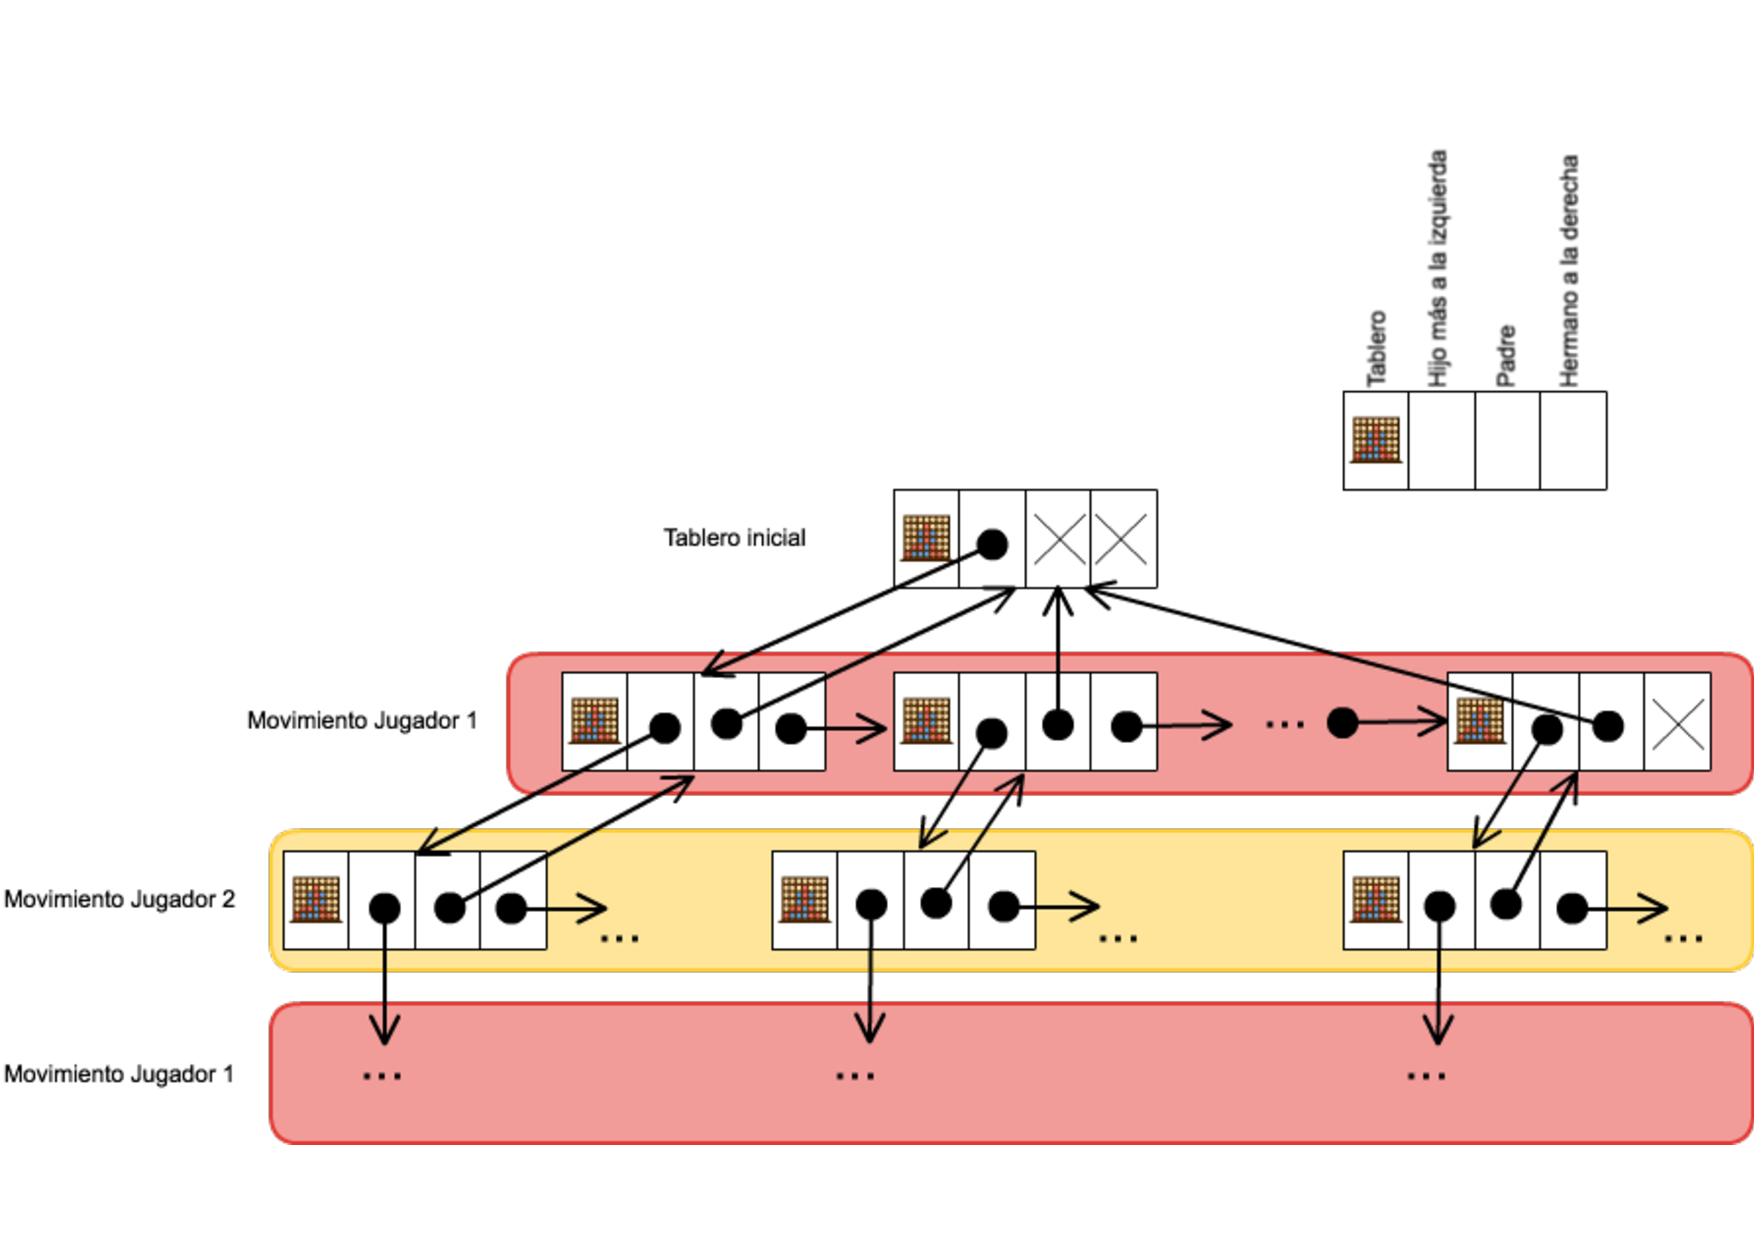
\includegraphics[width=12cm]{connect4-tree}
\caption{Estructura interna de un T\+DA Árbol General para representar el espacio de soluciones de Conecta 4}
\end{DoxyImage}







\begin{DoxyImage}
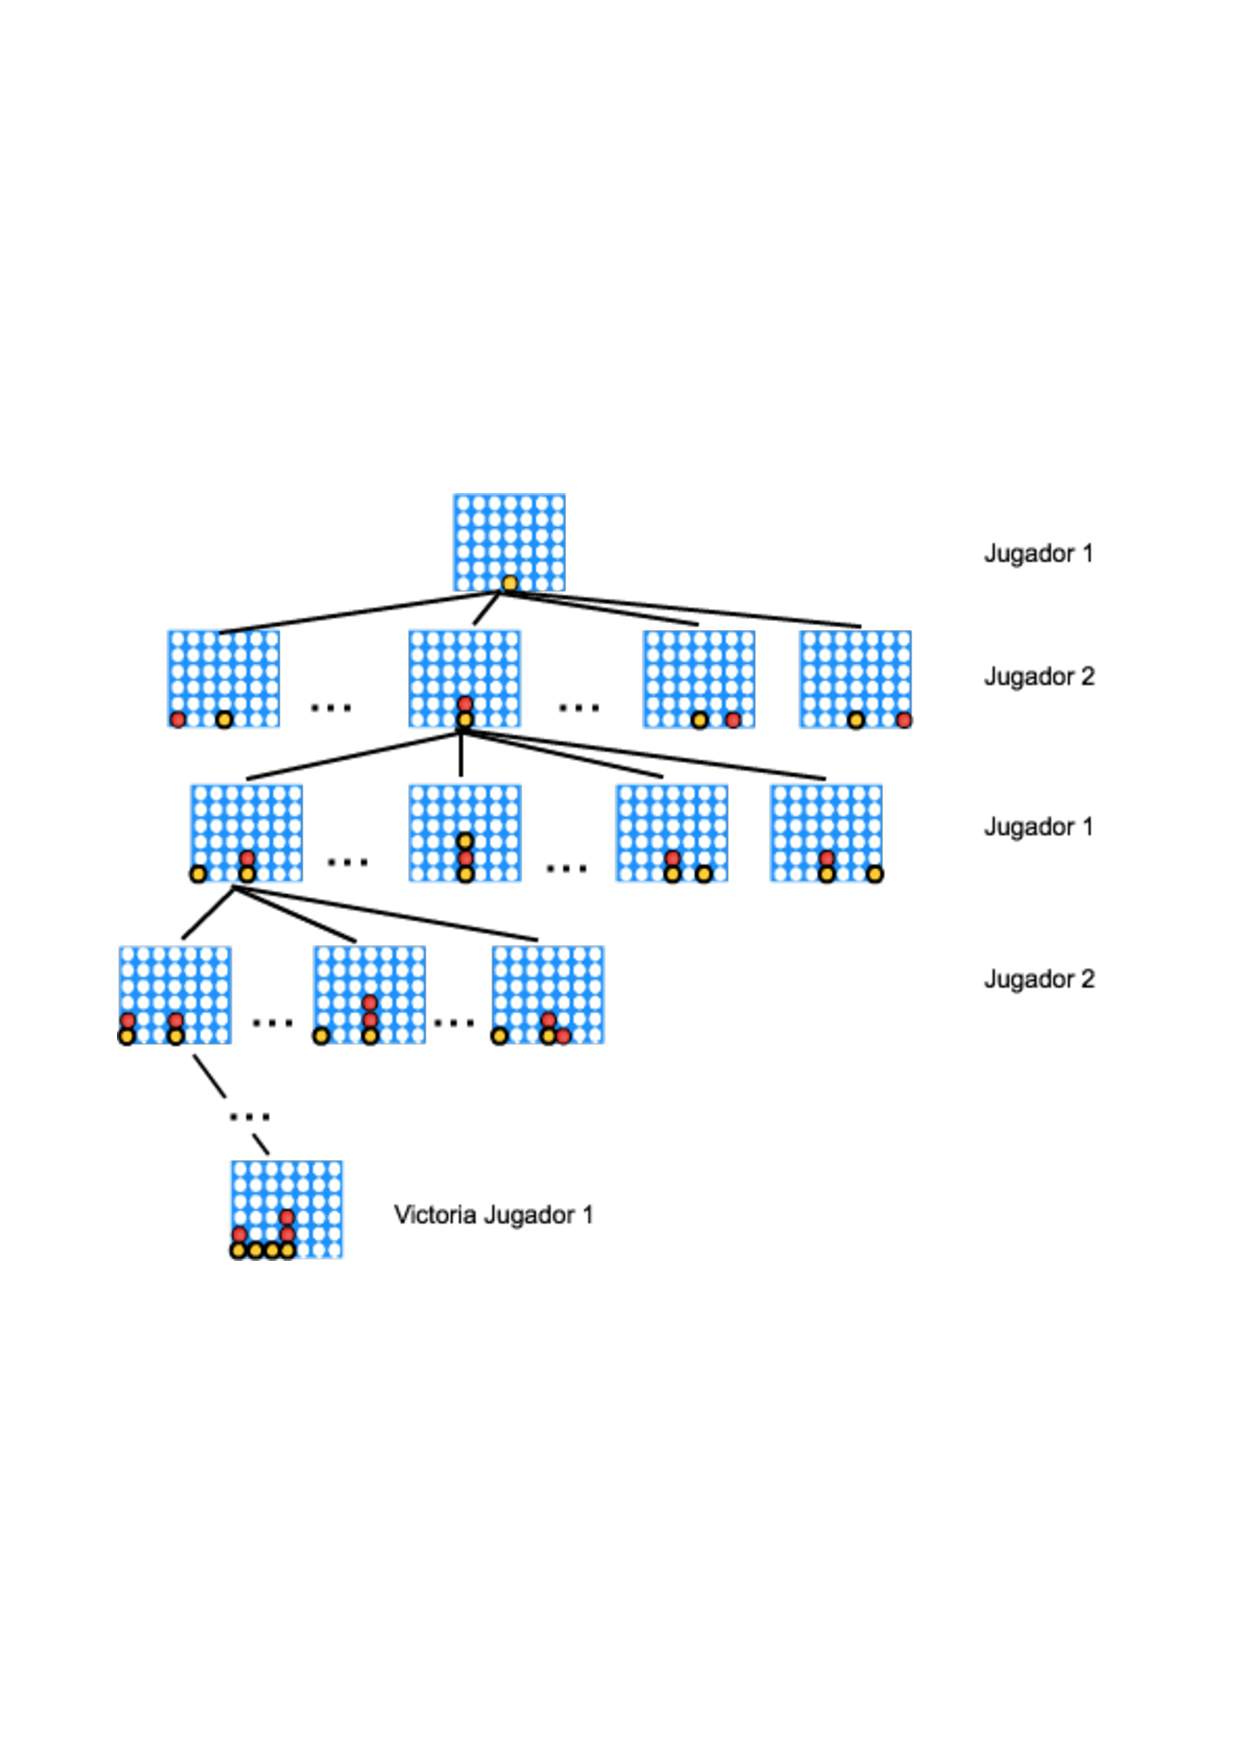
\includegraphics[width=12cm]{connect4-tree-YR}
\caption{Detalle de posibles movimientos en el espacio de soluciones de Conecta 4}
\end{DoxyImage}


El tamaño real de un tablero de Conecta 4 es de 6 filas x 7 columnas, con lo que cada nodo del árbol tiene hasta 7 hijos. Si una columna del tablero estuviera completa, habría menos movimientos posibles y por tanto menos hijos para ese nodo. Los nodos en los que la partida ya está resuelta (por victoria de uno de los jugadores o por no quedar movimientos posibles) serían los nodos hoja del árbol.

De este modo, en el primer nivel del árbol (considerando 1 turno desde el tablero actual), almacenaríamos hasta 7 jugadas posibles o tableros diferentes. En el segundo nivel (considerando 2 turnos desde el actual), almacenaríamos hasta 7$^\wedge$2 tableros posibles. En el tercero, hasta 7$^\wedge$3. Y así sucesivamente. El estudiante debe ser consciente del coste de almacenar y recorrer este volumen de tableros para implementar métricas de recomendación de movimientos que sean viables (coste razonable en tiempo y memoria). Por ejemplo, se recomienda implementar métricas que utilicen un árbol de movimientos para los próximos N turnos desde el tablero actual, donde N queda a elección del estudiante, para acotar el consumo en tiempo y memoria de la implementación de estas métricas.

Además, a medida que el juego va avanzando, se recomienda reutilizar las ramas del árbol de soluciones que siguen siendo posibles y utilizar mecanismos de poda (ya implementados en el T\+DA \hyperlink{classArbolGeneral}{Arbol\+General}) para liberar espacio en memoria eliminando las ramas con movimientos que no se han tomado.

En esta práctica, el estudiante deberá proponer e implementar distintas métricas para guiar la decisión del jugador automático, representando todas las jugadas posibles para los próximos N turnos utilizando un T.\+D.\+A. Árbol General.\hypertarget{index_tareas}{}\subsection{Tareas a realizar}\label{index_tareas}
Se proprocionan\+:
\begin{DoxyEnumerate}
\item T.\+D.\+A. \hyperlink{classTablero}{Tablero}\+: representación del tablero de Conecta 4. Un objeto tablero representa un instante dado de una partida del Conecta 4, es decir, la disposición de las fichas de ambos jugadores sobre el tablero y el turno del jugador al que le corresponde hacer el próximo movimiento.
\item T.\+D.\+A. \hyperlink{classMando}{Mando}\+: representación gráfica del tablero de Conecta 4. Incluye la gestión de Entrada/\+Salida que permite jugar a Conecta 4 de forma interactiva.
\item T.\+D.\+A. \hyperlink{classArbolGeneral}{Arbol\+General}.
\end{DoxyEnumerate}

Se deberán llevar a cabo las siguientes tareas\+:


\begin{DoxyEnumerate}
\item Construir el T.\+D.\+A. Conecta4, que almacena todos los tableros posibles de Conecta 4 generados en los próximos N turnos a partir de un tablero inicial utilizando las clases T.\+D.\+A. \hyperlink{classArbolGeneral}{Arbol\+General} y T.\+D.\+A. \hyperlink{classTablero}{Tablero}.
\item Definir los métodos del T.\+D.\+A. Conecta4 para la solución de los problemas propuestos, en particular, para la implementación de un jugador automático.
\item Probar los módulos con programas test. Se puede usar la S\+TL en todos los módulos excepto en la implementación del T\+DA \hyperlink{classArbolGeneral}{Arbol\+General}.
\end{DoxyEnumerate}

A continuación se detallan los programas que se deberán desarrollar.\hypertarget{index_jugador_automatico}{}\subsection{Implementar un jugador automático}\label{index_jugador_automatico}
Conecta 4 es un juego de estrategia abstracta donde los contrincantes disponen de información perfecta \mbox{[}Conecta4\mbox{]}. Por norma general, el primer jugador tiene más posibilidades de ganar si introduce la primera ficha en la columna central. Si lo hace en las contiguas se puede forzar un empate, mientras que si la mete en las más alejadas del centro su rival puede vencerle con mayor facilidad. Existen libros y webs donde se explican las mejores estrategias para ganar en el Conecta 4, por ejemplo puede consultarse \mbox{[}Allen13\mbox{]}.

El estudiante debe implementar distintas \char`\"{}métricas\char`\"{} que permitan al jugador automático decidir qué movimiento realizar dada una disposición del tablero. Las métricas implementadas analizarán el espacio de soluciones posible a partir del tablero actual para evaluar cuál es el movimiento más beneficioso para el jugador automático (esto es, el movimiento que más aumente las expectativas de ganar la partida). La calidad de estas métricas dependerá, en parte, de la cantidad de información de que dispongan. De este modo, una métrica que sólo considere dos niveles en profundidad a partir del tablero actual (esto es, todos los movimientos posibles del jugador y todas las repuestas inmediatas del rival) tendrá más limitaciones que una métrica que disponga de todo el árbol de soluciones a partir del tablero actual. Evidentemente, la contrapartida es que una métrica que dispone de todo el árbol de soluciones requiere de un alto consumo en memoria y en tiempo de cómputo (según el tamaño del tablero, almacenar todo el árbol de soluciones puede ser directamente inviable). De este modo, se propone diseñar distintas métricas utilizando un árbol de soluciones con N niveles en profundidad a partir del tablero actual, donde N es variable y su elección se deja al estudiante.

El estudiante debe implementar la clase T\+DA Conecta4 utilizando como tipo rep. el T\+DA. \hyperlink{classArbolGeneral}{Arbol\+General} para representar el espacio de soluciones con profundidad N e implementar distintas métricas que, haciendo uso de esta representación del espacio de soluciones, recomienden un movimiento al jugador automático. Anteriormente se ha descrito una posible métrica inicial que sólo requiere explorar un nivel del espacio de soluciones\+: evaluar si alguno de los movimientos posibles para el jugador automático produce directamente un tablero donde el jugador automático consigue 4 en línea (y, por tanto, gana la partida) o evita un 4 en línea del rival (y, por tanto, evita perder la partida). Otra métrica sencilla que requiere explorar todo el árbol de búsqueda hasta profundidad N consiste en hacer recuento de cuántos nodos a profundidad $<$=N son favorables/desfavorables (victorias/empates/derrotas) al jugador automático para cada nodo hijo del tablero actual, de modo que el hijo con mejores métricas indicará el mejor movimiento posible. Otras métricas más sofisticadas podrían explorar este espacio de búsqueda para considerar no sólo victorias o derrotas, sino también recontar el número de secuencias de tres/dos fichas del jugador automático no rodeadas por fichas del rival en cada uno de los tableros.

Es importante destacar que, para aliviar el costo de almacenamiento de las métricas basadas en árboles de búsqueda, una vez realizado un movimiento, el árbol debe podarse para eliminar los nodos asociados a movimientos alternativos que finalmente no fueron tomados. El T\+DA \hyperlink{classArbolGeneral}{Arbol\+General} incluye métodos de poda facilitan esta tarea.

El estudiante tiene libertad para implementar las métricas sugeridas o cualquier otra para guiar los movimientos del jugador automático. La documentación final a entregar debe recoger una descripción completa de cada métrica implementada y una justificación de sus resultados. Se valorará la dificultad para batir al jugador automático guiado por las métricas implementadas por el estudiante.

En la siguiente sección se detalla cómo implementar este programa principal para jugar a Conecta 4.\hypertarget{index_partida}{}\subsection{Implementar una partida de Conecta 4}\label{index_partida}
Se adjunta un programa de ejemplo ({\ttfamily src/conecta4.\+cpp}) que utiliza los T\+DA \hyperlink{classTablero}{Tablero} y T\+DA \hyperlink{classMando}{Mando} para implementar una partida de Conecta 4 interactiva entre dos jugadores (no automáticos). Nótese que este programa va pidiendo por teclado sucesivamente cada movimiento de ambos jugadores, y no hace uso del T\+DA \hyperlink{classArbolGeneral}{Arbol\+General} (no representa el espacio de soluciones posibles para emitir recomendaciones sobre el mejor movimiento o tomar decisiones automáticas).


\begin{DoxyCode}
\textcolor{preprocessor}{#include <iostream>}
\textcolor{preprocessor}{#include <vector>}
\textcolor{preprocessor}{#include <ctime>}
\textcolor{preprocessor}{#include <cstdlib>}
\textcolor{preprocessor}{#include <stdio.h>}
\textcolor{preprocessor}{#include <unistd.h>}
\textcolor{preprocessor}{#include <termio.h>}         \textcolor{comment}{// Linux/Windows users}
\textcolor{comment}{//#include <termios.h>      // Mac OSX users}

\textcolor{preprocessor}{#include "\hyperlink{ArbolGeneral_8h}{ArbolGeneral.h}"}
\textcolor{preprocessor}{#include "\hyperlink{tablero_8h}{tablero.h}"}
\textcolor{preprocessor}{#include "\hyperlink{mando_8h}{mando.h}"}

\textcolor{keyword}{using namespace }\hyperlink{namespacestd}{std};

\textcolor{comment}{// Captura el caracter pulsado por teclado (sin necesidad de pulsar, a continuación, Enter).}
\textcolor{comment}{// Devuelve: Caracter pulsado.}

\textcolor{keywordtype}{char} getch() \{
 ...
\}

\textcolor{comment}{// Imprime en pantalla el tablero completo, con el mando y el jugador.}
\textcolor{comment}{// t : Tablero que se va a imprimir.}
\textcolor{comment}{// m : Mando indicando la posición del jugador.}

\textcolor{keywordtype}{void} imprimeTablero(\hyperlink{classTablero}{Tablero} & t, \hyperlink{classMando}{Mando} & m)\{
    cout << m.\hyperlink{classMando_aaf8c918ecbce5c8173fcf40e04c8b0b7}{GetJugador}() << endl;
    cout << t ;
    cout << m.\hyperlink{classMando_abcc813b0881e56ed976eea2ce6b7fd12}{GetBase}() << endl;
    cout << m.\hyperlink{classMando_a7e02a04343208f949a88e720ba63a281}{GetMando}() << endl;
\}


\textcolor{comment}{// Implementa el desarrollo de una partida de Conecta 4 con dos jugadores humanos}
\textcolor{comment}{// Devuelve: identificador (int) del jugador que gana la partida}
\textcolor{keywordtype}{int} jugar\_partida() \{

    \hyperlink{classTablero}{Tablero} tablero(5, 7);      \textcolor{comment}{//Tablero 5x7}
    \hyperlink{classMando}{Mando} mando(tablero);       \textcolor{comment}{//Mando para controlar E/S de tablero}
    \textcolor{keywordtype}{char} c = 1;
    \textcolor{keywordtype}{int} quienGana = tablero.quienGana();
    \textcolor{comment}{//mientras no haya ganador y no se pulse tecla de terminación}
    \textcolor{keywordflow}{while}(c != \hyperlink{classMando_a3c4e7465d5b25fcaf8f3b50b444421a3}{Mando::KB\_ESCAPE} && quienGana == 0) \{
        system(\textcolor{stringliteral}{"clear"});
        mando.actualizarJuego(c, tablero);  \textcolor{comment}{// actualiza tablero según comando c }
        imprimeTablero(tablero, mando);     \textcolor{comment}{// muestra tablero y mando en pantalla}
        quienGana = tablero.quienGana();    \textcolor{comment}{// hay ganador?}
        \textcolor{keywordflow}{if}(quienGana==0) c = getch();       \textcolor{comment}{// Capturamos la tecla pulsada.    }
    \}

    \textcolor{keywordflow}{return} tablero.quienGana();
\}

\textcolor{keywordtype}{int} main(\textcolor{keywordtype}{int} argc, \textcolor{keywordtype}{char} *argv[])\{
    \textcolor{keywordtype}{int} ganador = jugar\_partida();
    cout << \textcolor{stringliteral}{"Ha ganado el jugador "} << ganador << endl;
\}  
\end{DoxyCode}


El estudiante debe implementar una partida de Conecta 4 en la que uno de los jugadores realiza sus movimientos automáticamente y el otro jugador introduce sus movimientos por teclado. Utilice el código de {\ttfamily src/conecta4.\+cpp} como base para programar este módulo. El programa debe permitir elegir cuál es el jugador que inicia la partida\+: el jugador automático o el humano.

Además, en caso de implementar distintas métricas que guían al jugador automático, el programa contará con un argumento entero que permite identificar la métrica utilizada por el jugador automático (métrica 1, métrica 2, y así sucesivamente). La métrica 1 será, por defecto, la que mejor resultados haya obtenido para el estudiante.

Finalmente, el programa debe también permitir definir el tamaño del tablero.

En resumen, el módulo a desarrollar por el estudiante debe tener los siguientes argumentos\+:

{\ttfamily prompt \%$>$ conecta4 $<$filas\+\_\+tablero$>$ $<$cols\+\_\+tablero$>$ $<$metrica$>$ $<$turno$>$}

Donde\+:


\begin{DoxyItemize}
\item {\ttfamily $<$filas\+\_\+tablero$>$, $<$cols\+\_\+tablero$>$}\+: especifica las dimensiones del tablero (por defecto, 4 en ambas opciones para tablero 4x4)
\item {\ttfamily $<$metrica$>$}\+: indica la métrica a utilizar para guiar al jugador automático. Comenzar a numerar con 1 y en adelante, en orden de mejores a peores resultados obtenidos con esa métrica para el jugador automático. 1 es la opción por defecto (la métrica con mejores resultados). 0 para que la partida se desarrolle entre dos jugadores humanos (sin jugador automático).
\item {\ttfamily $<$turno$>$} indica qué jugador tiene el primer turno\+:
\begin{DoxyItemize}
\item 1\+: primer turno para el jugador humano
\item 2\+: primer turno para el jugador automático
\end{DoxyItemize}
\end{DoxyItemize}\hypertarget{index_ArbolGeneral}{}\subsection{Manejo del T.\+D.\+A. Arbol\+General}\label{index_ArbolGeneral}
Se adjunta un programa de ejemplo ({\ttfamily src/arboltablero\+\_\+test.\+cpp}) en el que se exhibe alguna funcionalidad asociada a los T\+DA \hyperlink{classTablero}{Tablero} y \hyperlink{classArbolGeneral}{Arbol\+General}. En este programa se crean distintos objetos \hyperlink{classTablero}{Tablero} con distintas jugadas posibles de Conecta 4 y una estructura \hyperlink{classArbolGeneral}{Arbol\+General} que almacena jerárquicamente estos tableros.

En particular, se muestra como\+:

Para T\+DA \hyperlink{classTablero}{Tablero}\+:
\begin{DoxyItemize}
\item crear de tableros con las dimensiones deseadas
\item colocar ficha para el jugador que dispone del turno
\item cambiar turno entre jugadores
\end{DoxyItemize}

Para T\+DA \hyperlink{classArbolGeneral}{Arbol\+General}\+:
\begin{DoxyItemize}
\item crear de árboles con T\+DA \hyperlink{classTablero}{Tablero} como nodos
\item obtener el nodo raiz de un \hyperlink{classArbolGeneral}{Arbol\+General}
\item insertar nodos como hijomasizquierda
\item insertar nodos como hermanoderecha
\item imprimir \hyperlink{classArbolGeneral}{Arbol\+General} en preorden
\item podar una rama del \hyperlink{classArbolGeneral}{Arbol\+General}
\end{DoxyItemize}


\begin{DoxyCode}
\textcolor{preprocessor}{#include <iostream>}
\textcolor{preprocessor}{#include "\hyperlink{ArbolGeneral_8h}{ArbolGeneral.h}"}
\textcolor{preprocessor}{#include "\hyperlink{tablero_8h}{tablero.h}"}
\textcolor{preprocessor}{#include <string>}

\textcolor{keyword}{using namespace }\hyperlink{namespacestd}{std};


\textcolor{keywordtype}{int} main(\textcolor{keywordtype}{int} argc, \textcolor{keywordtype}{char} *argv[])\{

  \textcolor{comment}{//Tablero vacío 5x7}
    \hyperlink{classTablero}{Tablero} tablero(5, 7);

    \textcolor{comment}{//Manualmente se insertan algunos movimientos: }
    tablero.colocarFicha(3);  \textcolor{comment}{//Jugador 1 inserta ficha en columna 3}
    tablero.cambiarTurno();
    tablero.colocarFicha(1);  \textcolor{comment}{//Jugador 2 inserta ficha en columna 1}
    tablero.cambiarTurno();
    tablero.colocarFicha(3);  \textcolor{comment}{//Jugador 1 inserta ficha en columna 3.}
    tablero.cambiarTurno();
    
    \textcolor{comment}{//Se muestra el tablero }
    cout << \textcolor{stringliteral}{"Tablero obtenido tras tres movimientos: \(\backslash\)n"}<<tablero; 

    \textcolor{comment}{//A partir de la situación actual del tablero, montamos un árbol para estudiar algunas posibilidades. }

    \textcolor{comment}{// Éste es el árbol que queremos montar: }
    \textcolor{comment}{//        tablero}
    \textcolor{comment}{//          |}
    \textcolor{comment}{//      |---------------|}
    \textcolor{comment}{//    tablero1      tablero2}
    \textcolor{comment}{//                      |}
    \textcolor{comment}{//                  tablero3}


    \textcolor{comment}{//Árbol 'partida', con 'tablero' como nodo raíz}
    \hyperlink{classArbolGeneral}{ArbolGeneral<Tablero>} partida(tablero);

    \textcolor{comment}{//Estudio opciones a partir de tablero: Jugador 2 coloca ficha en columna 1. (tablero1)}
    \hyperlink{classTablero}{Tablero} tablero1(tablero);          \textcolor{comment}{//tablero queda sin modificar}
    tablero1.colocarFicha(1);   
    \hyperlink{classArbolGeneral}{ArbolGeneral<Tablero>} arbol1 (tablero1);  \textcolor{comment}{//creo árbol con un nodo (tablero1)}

    \textcolor{comment}{//Otra opción: Jugador 2 coloca ficha en columna 2. (tablero2)}
    \hyperlink{classTablero}{Tablero} tablero2(tablero);          \textcolor{comment}{//tablero queda sin modificar}
    tablero2.colocarFicha(2);
    \hyperlink{classArbolGeneral}{ArbolGeneral<Tablero>} arbol2(tablero2);   \textcolor{comment}{//creo árbol con un nodo}

    \textcolor{comment}{// Sobre la última opción, ahora contemplo la posibilidad de que }
    \textcolor{comment}{//  Jugador 1 coloque ficha también en columna 2. }
    tablero2.cambiarTurno();          \textcolor{comment}{//modifico tablero2 (esta modificación sería tablero3)}
    tablero2.colocarFicha(2); 
    \hyperlink{classArbolGeneral}{ArbolGeneral<Tablero>} arbol3 (tablero2);  \textcolor{comment}{//creo árbol con un nodo}
    arbol2.insertar\_hijomasizquierda(arbol2.raiz(), arbol3);  \textcolor{comment}{//añado este árbol como hijo de arbol2}

    \textcolor{comment}{// Inserto arbol1 y arbol2 como hijos de partida. }
    \textcolor{comment}{// arbol1 es el hijo más a la izquierda y arbol2 es hermano a la derecha de arbol1}
  
    \textcolor{comment}{//  Forma de hacerlo A: inserto varios hijomasizquierda en el orden inverso al deseado}
    \textcolor{comment}{//  partida.insertar\_hijomasizquierda(partida.raiz(), arbol2);}
    \textcolor{comment}{//  partida.insertar\_hijomasizquierda(partida.raiz(), arbol1);  //hijomasizquierda desplaza al anterior
       a la derecha}
  
    \textcolor{comment}{// Forma de hacerlo B: inserto un hijomasizquierda y hermanoderecha}
    partida.insertar\_hijomasizquierda(partida.raiz(), arbol1);              \textcolor{comment}{//inserto un hijomasizquierda}
    partida.insertar\_hermanoderecha(partida.hijomasizquierda(partida.raiz()), arbol2);  \textcolor{comment}{//le inserto un
       hermanoderecha}
    

    \textcolor{comment}{// Recorremos en preorden para comprobar el arbol 'partida' resultante}
    cout << \textcolor{stringliteral}{"\(\backslash\)nÁrbol en preorden: \(\backslash\)n"}<<endl; 
    partida.recorrer\_preorden();

    \textcolor{comment}{// Podamos el hijomasizquierda y recorremos en preorden: }
    \hyperlink{classArbolGeneral}{ArbolGeneral<Tablero>} rama\_podada;
    partida.\hyperlink{classArbolGeneral_a7f2fa2d9be4af4b7be1c334819a04c39}{podar\_hijomasizquierda}(partida.raiz(), rama\_podada);

    cout << \textcolor{stringliteral}{"\(\backslash\)nRecorrido preorden después de podar hijomasizquierda: \(\backslash\)n"}<<endl; 
    partida.recorrer\_preorden();

    \textcolor{keywordflow}{return} 0;
\}
\end{DoxyCode}


El estudiante deber revisar detenidamente este código y la documentación completa asociada a las clases T\+DA \hyperlink{classTablero}{Tablero} y T\+DA \hyperlink{classArbolGeneral}{Arbol\+General} para familiarizarse con su manejo y sacarles el máximo partido para la implementación del T.\+D.\+A. Conecta4.\hypertarget{index_recomendaciones}{}\subsection{Recomendaciones}\label{index_recomendaciones}

\begin{DoxyItemize}
\item Analice con detenimiento la documentación de las clases proporcionadas\+: T.\+D.\+A. \hyperlink{classArbolGeneral}{Arbol\+General}, T.\+D.\+A. \hyperlink{classTablero}{Tablero} y T.\+D.\+A. \hyperlink{classMando}{Mando}. Parte importante del esfuerzo que debe realizar en esta práctica es entender cómo debe utilizar estas clases para su proyecto. Esta práctica es habitual en empresas\+: para el desarrollo de un proyecto se cuenta con parte del código desarrollado previamente por otro equipo.
\item Para acotar el espacio de búsqueda y el tamaño de los objetos \hyperlink{classArbolGeneral}{Arbol\+General}, comience el desarrollo de su proyecto considerando tableros más pequeños (por ejemplo, 4x4). Cuando el funcionamiento sea correcto, amplíe progresivamente el tamaño de los tableros. Del mismo modo, considere con cautela la profundidad máxima N que va a explorar en el árbol de soluciones. Comience con un valor bajo de N y estudie hasta qué valor de N (depende del tamaño del tablero) es viable el cálculo de sus métricas.
\end{DoxyItemize}\hypertarget{index_entrega}{}\subsection{Entrega}\label{index_entrega}
El estudiante deberá empaquetar todos los archivos relacionados en el proyecto en un archivo con nombre “conecta4.\+tgz” y entregarlo antes de la fecha que se publicará en la página web de la asignatura. Tenga en cuenta que no se incluirán ficheros objeto, ni ejecutables, ni la carpeta datos. Es recomendable que haga una “limpieza” para eliminar los archivos temporales o que se puedan generar a partir de los fuentes. El estudiante debe incluir el archivo Makefile para realizar la compilación. Tenga en cuenta que los archivos deben estar distribuidos en directorios\+:

conecta4
\begin{DoxyItemize}
\item Makefile
\item include -- Carpeta con ficheros de cabecera (.h)
\item src --Carpeta con código fuente (.cpp)
\item doc --Carpeta con Documentación
\item obj -- Carpeta para código objeto (.o)
\item bin -- Carpeta para ejecutables
\item datos -- Carpeta para ficheros de datos
\end{DoxyItemize}

Para realizar la entrega, en primer lugar, realice la limpieza de archivos que no se incluirán en ella, y sitúese en la carpeta superior (en el mismo nivel de la carpeta \char`\"{}conecta4\char`\"{}) para ejecutar\+: 
\begin{DoxyCode}
prompt% tar zcv conecta4.tgz conecta4
\end{DoxyCode}
 tras lo cual, dispondrá de un nuevo archivo conecta4.\+tgz que contiene la carpeta conecta4 así como todas las carpetas y archivos que cuelgan de ella.

La fecha límite de entrega es el día 22 de Enero de 2017 a las 23\+:59.\hypertarget{index_referencias}{}\subsection{Referencias}\label{index_referencias}
\mbox{[}Allen13\mbox{]} James D. Allen. \char`\"{}\+Expert Play in Connect-\/\+Four\char`\"{} (en inglés). Archivado desde el original el 4 de noviembre de 2015. \href{http://web.archive.org/web/20141125065033/http://homepages.cwi.nl/~tromp/c4.html}{\tt http\+://web.\+archive.\+org/web/20141125065033/http\+://homepages.\+cwi.\+nl/$\sim$tromp/c4.\+html}

\mbox{[}Conecta4\mbox{]} \href{https://es.wikipedia.org/wiki/Conecta_4}{\tt https\+://es.\+wikipedia.\+org/wiki/\+Conecta\+\_\+4}

\mbox{[}G\+A\+R06b\mbox{]} Garrido, A. Fdez-\/\+Valdivia, J. \char`\"{}\+Abstracción y estructuras de datos en C++\char`\"{}. Delta publicaciones, 2006. 
\section{Rep del T\+DA Arbol General}
\label{repConjunto}
\hypertarget{repConjunto}{}
\hypertarget{repConjunto_invConjunto}{}\subsection{Invariante de la representación}\label{repConjunto_invConjunto}
Sea {\itshape T} un Árbol General sobre el tipo {\itshape Tbase}. Entonces el invariante de la representación es

Si {\itshape T} es vacío, entonces T.\+laraiz vale 0. Si no\+:
\begin{DoxyItemize}
\item T.\+laraiz-\/$>$padre = 0 y
\item $ \forall $ n nodo de {\itshape T}, n-\/$>$izqda $ \neq $ n-\/$>$drch y
\item $ \forall $ n, m nodos de {\itshape T}, si n-\/$>$izqda = m, entonces m-\/$>$padre = n y
\item Número de elementos = número elementos de la raiz, donde N(n) = 1 + N(n-\/$>$izqda) + (N-\/$>$drcha), con N(0) = 0.
\end{DoxyItemize}\hypertarget{repConjunto_faConjunto}{}\subsection{Función de abstracción}\label{repConjunto_faConjunto}
Sea {\itshape T} un Árbol General sobre el tipo {\itshape Tbase}. Entonces, si lo denotamos también Árbol(T.\+laraiz), es decir, como el árbol que cuelga de su raíz, entonces este árbol del conjunto de valores en la representación se aplica al árbol.

\{ T.\+laraiz-\/$>$etiqueta, \{Arbol(T.\+laraiz-\/$>$izqda)\}, \{Arbol(T.\+laraiz-\/$>$drcha)\} \}

donde \{0\} es el árbol vacío. 
\section{Índice de clases}
\subsection{Lista de clases}
Lista de las clases, estructuras, uniones e interfaces con una breve descripción\+:\begin{DoxyCompactList}
\item\contentsline{section}{\hyperlink{classArbolGeneral}{Arbol\+General$<$ Tbase $>$} \\*T.\+D.\+A. \hyperlink{classArbolGeneral}{Arbol\+General} }{\pageref{classArbolGeneral}}{}
\item\contentsline{section}{\hyperlink{classArbolGeneral_1_1inorden__iterador}{Arbol\+General$<$ Tbase $>$\+::inorden\+\_\+iterador} }{\pageref{classArbolGeneral_1_1inorden__iterador}}{}
\item\contentsline{section}{\hyperlink{classMando}{Mando} \\*T\+DA \hyperlink{classMando}{Mando} }{\pageref{classMando}}{}
\item\contentsline{section}{\hyperlink{structArbolGeneral_1_1nodo}{Arbol\+General$<$ Tbase $>$\+::nodo} \\*Rep\+Conjunto Rep del T\+DA \hyperlink{classArbolGeneral}{Arbol\+General} }{\pageref{structArbolGeneral_1_1nodo}}{}
\item\contentsline{section}{\hyperlink{classArbolGeneral_1_1postorden__iterador}{Arbol\+General$<$ Tbase $>$\+::postorden\+\_\+iterador} }{\pageref{classArbolGeneral_1_1postorden__iterador}}{}
\item\contentsline{section}{\hyperlink{classArbolGeneral_1_1preorden__iterador}{Arbol\+General$<$ Tbase $>$\+::preorden\+\_\+iterador} }{\pageref{classArbolGeneral_1_1preorden__iterador}}{}
\item\contentsline{section}{\hyperlink{classArbolGeneral_1_1reverse__preorden__iterador}{Arbol\+General$<$ Tbase $>$\+::reverse\+\_\+preorden\+\_\+iterador} }{\pageref{classArbolGeneral_1_1reverse__preorden__iterador}}{}
\item\contentsline{section}{\hyperlink{classTablero}{Tablero} \\*T.\+D.\+A. \hyperlink{classTablero}{Tablero} }{\pageref{classTablero}}{}
\end{DoxyCompactList}

\section{Indice de archivos}
\subsection{Lista de archivos}
Lista de todos los archivos con descripciones breves\+:\begin{DoxyCompactList}
\item\contentsline{section}{include/\hyperlink{ArbolGeneral_8h}{Arbol\+General.\+h} }{\pageref{ArbolGeneral_8h}}{}
\item\contentsline{section}{include/\hyperlink{Conecta4_8h}{Conecta4.\+h} }{\pageref{Conecta4_8h}}{}
\item\contentsline{section}{include/\hyperlink{mando_8h}{mando.\+h} }{\pageref{mando_8h}}{}
\item\contentsline{section}{include/\hyperlink{tablero_8h}{tablero.\+h} }{\pageref{tablero_8h}}{}
\end{DoxyCompactList}

\section{Documentación de las clases}
\hypertarget{classArbolGeneral}{}\subsection{Referencia de la plantilla de la Clase Arbol\+General$<$ Tbase $>$}
\label{classArbolGeneral}\index{Arbol\+General$<$ Tbase $>$@{Arbol\+General$<$ Tbase $>$}}


T.\+D.\+A. \hyperlink{classArbolGeneral}{Arbol\+General}.  




{\ttfamily \#include $<$Arbol\+General.\+h$>$}

\subsubsection*{Clases}
\begin{DoxyCompactItemize}
\item 
class \hyperlink{classArbolGeneral_1_1inorden__iterador}{inorden\+\_\+iterador}
\item 
struct \hyperlink{structArbolGeneral_1_1nodo}{nodo}
\begin{DoxyCompactList}\small\item\em nodo \end{DoxyCompactList}\item 
class \hyperlink{classArbolGeneral_1_1postorden__iterador}{postorden\+\_\+iterador}
\item 
class \hyperlink{classArbolGeneral_1_1preorden__iterador}{preorden\+\_\+iterador}
\item 
class \hyperlink{classArbolGeneral_1_1reverse__preorden__iterador}{reverse\+\_\+preorden\+\_\+iterador}
\end{DoxyCompactItemize}
\subsubsection*{Tipos públicos}
\begin{DoxyCompactItemize}
\item 
typedef struct \hyperlink{structArbolGeneral_1_1nodo}{nodo} $\ast$ \hyperlink{classArbolGeneral_a12cc1b74a9095d89bc7334290d332f7a}{Nodo}
\begin{DoxyCompactList}\small\item\em Tipo Nodo. \end{DoxyCompactList}\end{DoxyCompactItemize}
\subsubsection*{Métodos públicos}
\begin{DoxyCompactItemize}
\item 
\hyperlink{classArbolGeneral_a2c792965befd8644246118a09a10123c}{Arbol\+General} ()
\begin{DoxyCompactList}\small\item\em Constructor por defecto. \end{DoxyCompactList}\item 
\hyperlink{classArbolGeneral_a8ddac1a024f05bee96f4c259fad76c4c}{Arbol\+General} (const Tbase \&e)
\begin{DoxyCompactList}\small\item\em Constructor de raíz. \end{DoxyCompactList}\item 
\hyperlink{classArbolGeneral_ad7926f03eb051b9691d57f4e508cad4d}{Arbol\+General} (const \hyperlink{classArbolGeneral}{Arbol\+General}$<$ Tbase $>$ \&v)
\begin{DoxyCompactList}\small\item\em Constructor de copias. \end{DoxyCompactList}\item 
\hyperlink{classArbolGeneral_a085c45825063913fb958b704f59033f3}{$\sim$\+Arbol\+General} ()
\begin{DoxyCompactList}\small\item\em Destructor. \end{DoxyCompactList}\item 
\hyperlink{classArbolGeneral}{Arbol\+General}$<$ Tbase $>$ \& \hyperlink{classArbolGeneral_aebd3723e9929b905445127a754a26759}{operator=} (const \hyperlink{classArbolGeneral}{Arbol\+General}$<$ Tbase $>$ \&v)
\begin{DoxyCompactList}\small\item\em Operador de asignación. \end{DoxyCompactList}\item 
void \hyperlink{classArbolGeneral_a84781986cd57390540600494303b0e9d}{Asigna\+Raiz} (const Tbase \&e)
\begin{DoxyCompactList}\small\item\em Asignar nodo raíz. \end{DoxyCompactList}\item 
\hyperlink{classArbolGeneral_a12cc1b74a9095d89bc7334290d332f7a}{Nodo} \hyperlink{classArbolGeneral_a7604d8f20552803253132bdaff134f18}{raiz} () const
\begin{DoxyCompactList}\small\item\em Raíz del árbol. \end{DoxyCompactList}\item 
\hyperlink{classArbolGeneral_a12cc1b74a9095d89bc7334290d332f7a}{Nodo} \hyperlink{classArbolGeneral_aa0b433b9afe680fbdf84f72493f92f68}{hijomasizquierda} (const \hyperlink{classArbolGeneral_a12cc1b74a9095d89bc7334290d332f7a}{Nodo} n) const
\begin{DoxyCompactList}\small\item\em Hijo más a la izquierda. \end{DoxyCompactList}\item 
\hyperlink{classArbolGeneral_a12cc1b74a9095d89bc7334290d332f7a}{Nodo} \hyperlink{classArbolGeneral_a33984e2259e92dc86a18b6ee1e89f251}{hermanoderecha} (const \hyperlink{classArbolGeneral_a12cc1b74a9095d89bc7334290d332f7a}{Nodo} n) const
\begin{DoxyCompactList}\small\item\em Hermano derecha. \end{DoxyCompactList}\item 
\hyperlink{classArbolGeneral_a12cc1b74a9095d89bc7334290d332f7a}{Nodo} \hyperlink{classArbolGeneral_a8c63cdc5b3c4fa9a5883567a19049423}{padre} (const \hyperlink{classArbolGeneral_a12cc1b74a9095d89bc7334290d332f7a}{Nodo} n) const
\begin{DoxyCompactList}\small\item\em Nodo padre. \end{DoxyCompactList}\item 
Tbase \& \hyperlink{classArbolGeneral_a69781940bd69c1e473e0c4b2495cd7a1}{etiqueta} (const \hyperlink{classArbolGeneral_a12cc1b74a9095d89bc7334290d332f7a}{Nodo} n)
\begin{DoxyCompactList}\small\item\em Etiqueta de un nodo. \end{DoxyCompactList}\item 
const Tbase \& \hyperlink{classArbolGeneral_affb3c52c9c82ff2d3c4b9a8b5499b91c}{etiqueta} (const \hyperlink{classArbolGeneral_a12cc1b74a9095d89bc7334290d332f7a}{Nodo} n) const
\begin{DoxyCompactList}\small\item\em Etiqueta de un nodo. \end{DoxyCompactList}\item 
void \hyperlink{classArbolGeneral_ad9fddc80b179cac8eddc113a048334c1}{asignar\+\_\+subarbol} (const \hyperlink{classArbolGeneral}{Arbol\+General}$<$ Tbase $>$ \&orig, const \hyperlink{classArbolGeneral_a12cc1b74a9095d89bc7334290d332f7a}{Nodo} nod)
\begin{DoxyCompactList}\small\item\em Copia subárbol. \end{DoxyCompactList}\item 
void \hyperlink{classArbolGeneral_a7f2fa2d9be4af4b7be1c334819a04c39}{podar\+\_\+hijomasizquierda} (\hyperlink{classArbolGeneral_a12cc1b74a9095d89bc7334290d332f7a}{Nodo} n, \hyperlink{classArbolGeneral}{Arbol\+General}$<$ Tbase $>$ \&dest)
\begin{DoxyCompactList}\small\item\em Podar subárbol hijo más a la izquierda. \end{DoxyCompactList}\item 
void \hyperlink{classArbolGeneral_a81282ccc37494f1e13042e06ea475fb6}{podar\+\_\+hermanoderecha} (\hyperlink{classArbolGeneral_a12cc1b74a9095d89bc7334290d332f7a}{Nodo} n, \hyperlink{classArbolGeneral}{Arbol\+General}$<$ Tbase $>$ \&dest)
\begin{DoxyCompactList}\small\item\em Podar subárbol hermano derecha. \end{DoxyCompactList}\item 
void \hyperlink{classArbolGeneral_acf95226edb2a4e4c7fba82aaa82d0ec9}{insertar\+\_\+hijomasizquierda} (\hyperlink{classArbolGeneral_a12cc1b74a9095d89bc7334290d332f7a}{Nodo} n, \hyperlink{classArbolGeneral}{Arbol\+General}$<$ Tbase $>$ \&rama)
\begin{DoxyCompactList}\small\item\em Insertar subárbol hijo más a la izquierda. \end{DoxyCompactList}\item 
void \hyperlink{classArbolGeneral_a855d44f14a9ef638f8dd46376fc2f961}{insertar\+\_\+hermanoderecha} (\hyperlink{classArbolGeneral_a12cc1b74a9095d89bc7334290d332f7a}{Nodo} n, \hyperlink{classArbolGeneral}{Arbol\+General}$<$ Tbase $>$ \&rama)
\begin{DoxyCompactList}\small\item\em Insertar subárbol hermano derecha. \end{DoxyCompactList}\item 
void \hyperlink{classArbolGeneral_a3ae21db42586b23ccc082aeb321db56f}{clear} ()
\begin{DoxyCompactList}\small\item\em Borra todos los elementos. \end{DoxyCompactList}\item 
int \hyperlink{classArbolGeneral_ae5f8e2a36299629c36b33e344b0d0c47}{size} () const
\begin{DoxyCompactList}\small\item\em Número de elementos. \end{DoxyCompactList}\item 
bool \hyperlink{classArbolGeneral_a9f4d947bee0af4ff4678accf263ea843}{empty} () const
\begin{DoxyCompactList}\small\item\em Vacío. \end{DoxyCompactList}\item 
int \hyperlink{classArbolGeneral_a6876f408388bbe7cead25c4caeb0ea72}{altura} (\hyperlink{classArbolGeneral_a12cc1b74a9095d89bc7334290d332f7a}{Nodo} t) const
\begin{DoxyCompactList}\small\item\em Altura de un nodo. \end{DoxyCompactList}\item 
void \hyperlink{classArbolGeneral_a9b498b5302c63aa8ad0cd847d77a6315}{reflejado} (\hyperlink{classArbolGeneral_a12cc1b74a9095d89bc7334290d332f7a}{Nodo} t)
\begin{DoxyCompactList}\small\item\em Arbol reflejado. \end{DoxyCompactList}\item 
bool \hyperlink{classArbolGeneral_a4d4f2b67b2b9b973b182da62ad548495}{operator==} (const \hyperlink{classArbolGeneral}{Arbol\+General}$<$ Tbase $>$ \&v) const
\begin{DoxyCompactList}\small\item\em Operador de comparación (igualdad) \end{DoxyCompactList}\item 
bool \hyperlink{classArbolGeneral_a9132b4a848ed7b112f279df79adf76d8}{operator!=} (const \hyperlink{classArbolGeneral}{Arbol\+General}$<$ Tbase $>$ \&v) const
\begin{DoxyCompactList}\small\item\em Operador de comparación (diferencia) \end{DoxyCompactList}\item 
void \hyperlink{classArbolGeneral_a5fd1c0acc26d4229042ecd9af6e3a24e}{recuperar\+\_\+arbol} (string preorden, string inorden, string postorden, \hyperlink{classArbolGeneral_a12cc1b74a9095d89bc7334290d332f7a}{Nodo} nuevo)
\begin{DoxyCompactList}\small\item\em Crea un arbol a partir de sus tres recorridos. \end{DoxyCompactList}\item 
\hyperlink{classArbolGeneral_1_1preorden__iterador}{preorden\+\_\+iterador} \hyperlink{classArbolGeneral_a7ddb1b199b106d0bff369019ec792bba}{beginpreorden} () const
\begin{DoxyCompactList}\small\item\em Comienzo de un iterador \hyperlink{classArbolGeneral_1_1preorden__iterador}{preorden\+\_\+iterador}. \end{DoxyCompactList}\item 
\hyperlink{classArbolGeneral_1_1preorden__iterador}{preorden\+\_\+iterador} \hyperlink{classArbolGeneral_a274d347915b21304bdd2b1014c9d0e47}{endpreorden} () const
\begin{DoxyCompactList}\small\item\em Final de un iterador \hyperlink{classArbolGeneral_1_1preorden__iterador}{preorden\+\_\+iterador}. \end{DoxyCompactList}\item 
void \hyperlink{classArbolGeneral_a41993789af53e60c86ec2031af533965}{recorrer\+\_\+preorden} () const
\begin{DoxyCompactList}\small\item\em Recorrido en preorden.  Muestra el recorrido del árbol en preorden usando iteradores. \end{DoxyCompactList}\item 
void \hyperlink{classArbolGeneral_a0a9d574133bfc5b80dc5136094692830}{recorrer\+\_\+preorden2} (\hyperlink{classArbolGeneral_a12cc1b74a9095d89bc7334290d332f7a}{Nodo} t) const
\begin{DoxyCompactList}\small\item\em Recorrido en preorden. \end{DoxyCompactList}\item 
void \hyperlink{classArbolGeneral_af9a135c995c5baf31400a07e03415fcf}{recorrer\+\_\+preorden\+\_\+al\+\_\+reves} () const
\begin{DoxyCompactList}\small\item\em Recorrido en preorden al reves.  Muestra el recorrido del árbol en preorden, pero al reves. Utilizando iteradores preorden. \end{DoxyCompactList}\item 
\hyperlink{classArbolGeneral_1_1reverse__preorden__iterador}{reverse\+\_\+preorden\+\_\+iterador} \hyperlink{classArbolGeneral_a93ed98e3c548151103e05b693444d3c3}{beginreverse\+\_\+preorden} () const
\begin{DoxyCompactList}\small\item\em Comienzo de un iterador \hyperlink{classArbolGeneral_1_1reverse__preorden__iterador}{reverse\+\_\+preorden\+\_\+iterador}. \end{DoxyCompactList}\item 
\hyperlink{classArbolGeneral_1_1reverse__preorden__iterador}{reverse\+\_\+preorden\+\_\+iterador} \hyperlink{classArbolGeneral_ace49548e1d382c65bab7b9df6b9ff353}{endreverse\+\_\+preorden} () const
\begin{DoxyCompactList}\small\item\em Final de un iterador \hyperlink{classArbolGeneral_1_1reverse__preorden__iterador}{reverse\+\_\+preorden\+\_\+iterador}. \end{DoxyCompactList}\item 
void \hyperlink{classArbolGeneral_a49e61a49ae143e325f408af7b3930751}{recorrer\+\_\+reverse\+\_\+preorden} () const
\begin{DoxyCompactList}\small\item\em Recorrido en preorden invertido.  Muestra el recorrido del árbol en preorden invertido usando iteradores. \end{DoxyCompactList}\item 
void \hyperlink{classArbolGeneral_a0a427c239f20f7ef0088848570f4095e}{recorrer\+\_\+reverse\+\_\+preorden\+\_\+al\+\_\+reves} () const
\begin{DoxyCompactList}\small\item\em Recorrido en preorden invertido, al reves.  Recorrido en preorden normal. \end{DoxyCompactList}\item 
\hyperlink{classArbolGeneral_1_1inorden__iterador}{inorden\+\_\+iterador} \hyperlink{classArbolGeneral_addc9cdf77ec43de8669989f18bfbb6fa}{begininorden} () const
\begin{DoxyCompactList}\small\item\em Comienzo de un iterador \hyperlink{classArbolGeneral_1_1inorden__iterador}{inorden\+\_\+iterador}. \end{DoxyCompactList}\item 
\hyperlink{classArbolGeneral_1_1inorden__iterador}{inorden\+\_\+iterador} \hyperlink{classArbolGeneral_aedd96d245784059fb2da2aa18e4a45a0}{endinorden} () const
\begin{DoxyCompactList}\small\item\em Final de un iterador \hyperlink{classArbolGeneral_1_1inorden__iterador}{inorden\+\_\+iterador}. \end{DoxyCompactList}\item 
void \hyperlink{classArbolGeneral_a2ef9f4a8e55d88e21eb6e9c41dda934f}{recorrer\+\_\+inorden} () const
\begin{DoxyCompactList}\small\item\em Recorrido en inorden.  Muestra el árbol recorriendolo en inorden usando iteradores. \end{DoxyCompactList}\item 
void \hyperlink{classArbolGeneral_acaf0169d0b147e0727d28c09edc62e28}{recorrer\+\_\+inorden2} (\hyperlink{classArbolGeneral_a12cc1b74a9095d89bc7334290d332f7a}{Nodo} t) const
\begin{DoxyCompactList}\small\item\em Recorrido en inorden. \end{DoxyCompactList}\item 
\hyperlink{classArbolGeneral_1_1postorden__iterador}{postorden\+\_\+iterador} \hyperlink{classArbolGeneral_a59f2bce358114242dcb07d4c7974cb2f}{beginpostorden} () const
\begin{DoxyCompactList}\small\item\em Primer elemento en postorden. \end{DoxyCompactList}\item 
\hyperlink{classArbolGeneral_1_1postorden__iterador}{postorden\+\_\+iterador} \hyperlink{classArbolGeneral_a7f63c88d6c944709d05bb753351c4be5}{endpostorden} () const
\begin{DoxyCompactList}\small\item\em Último elmento. \end{DoxyCompactList}\item 
void \hyperlink{classArbolGeneral_a55ea6b4722f498562d1226d9e8d4c8f9}{recorrer\+\_\+postorden} () const
\begin{DoxyCompactList}\small\item\em Recorrido en postorden.  Recorre el árbol en postorden. Desde la raíz. \end{DoxyCompactList}\item 
void \hyperlink{classArbolGeneral_aafec68ff2d9979b4a1fe860c2af622a7}{recorrer\+\_\+postorden2} (\hyperlink{classArbolGeneral_a12cc1b74a9095d89bc7334290d332f7a}{Nodo} t) const
\begin{DoxyCompactList}\small\item\em Recorrido postorden. \end{DoxyCompactList}\item 
void \hyperlink{classArbolGeneral_ac6291959a1b891dc19e29c5ec9916417}{recorrer\+\_\+por\+\_\+niveles} (\hyperlink{classArbolGeneral_a12cc1b74a9095d89bc7334290d332f7a}{Nodo} t) const
\begin{DoxyCompactList}\small\item\em Recorrido por niveles. \end{DoxyCompactList}\end{DoxyCompactItemize}
\subsubsection*{Métodos privados}
\begin{DoxyCompactItemize}
\item 
void \hyperlink{classArbolGeneral_aba5f46f715343b9ee4952c30da065f8f}{destruir} (\hyperlink{structArbolGeneral_1_1nodo}{nodo} $\ast$n)
\begin{DoxyCompactList}\small\item\em Destruye el subárbol. \end{DoxyCompactList}\item 
void \hyperlink{classArbolGeneral_a79f31cbba599abea7ab8b2f4ac7bef91}{copiar} (\hyperlink{structArbolGeneral_1_1nodo}{nodo} $\ast$\&dest, \hyperlink{structArbolGeneral_1_1nodo}{nodo} $\ast$orig)
\begin{DoxyCompactList}\small\item\em Copia un subárbol. \end{DoxyCompactList}\item 
int \hyperlink{classArbolGeneral_a9f8c2adf966a9fe3155921bb849d3999}{contar} (const \hyperlink{structArbolGeneral_1_1nodo}{nodo} $\ast$n) const
\begin{DoxyCompactList}\small\item\em Cuenta el número de nodos. \end{DoxyCompactList}\item 
int \hyperlink{classArbolGeneral_a4842a2c8abe5979ef0a32fda99ea493d}{contar\+\_\+\+Hijos} (\hyperlink{structArbolGeneral_1_1nodo}{nodo} $\ast$n) const
\begin{DoxyCompactList}\small\item\em Cuenta el número de hijos. \end{DoxyCompactList}\item 
bool \hyperlink{classArbolGeneral_a645db91bf075b5a01e0cd5a072cedf1e}{soniguales} (const \hyperlink{structArbolGeneral_1_1nodo}{nodo} $\ast$n1, const \hyperlink{structArbolGeneral_1_1nodo}{nodo} $\ast$n2) const
\begin{DoxyCompactList}\small\item\em Comprueba igualdad de dos subárboles. \end{DoxyCompactList}\item 
void \hyperlink{classArbolGeneral_abac6b7ce1205ab23ad535a431e3038c7}{escribe\+\_\+arbol} (std\+::ostream \&out, \hyperlink{structArbolGeneral_1_1nodo}{nodo} $\ast$nod) const
\begin{DoxyCompactList}\small\item\em Escribe un subárbol. \end{DoxyCompactList}\item 
void \hyperlink{classArbolGeneral_a73927127a9f5c4e96eccb615ee09077a}{lee\+\_\+arbol} (std\+::istream \&in, \hyperlink{structArbolGeneral_1_1nodo}{nodo} $\ast$\&nod)
\begin{DoxyCompactList}\small\item\em Lee un subárbol. \end{DoxyCompactList}\end{DoxyCompactItemize}
\subsubsection*{Atributos privados}
\begin{DoxyCompactItemize}
\item 
struct \hyperlink{structArbolGeneral_1_1nodo}{nodo} $\ast$ \hyperlink{classArbolGeneral_a14a859dc79b8df4d5a77b5c871713c9e}{laraiz}
\begin{DoxyCompactList}\small\item\em Puntero a la raíz. \end{DoxyCompactList}\end{DoxyCompactItemize}
\subsubsection*{Amigas}
\begin{DoxyCompactItemize}
\item 
{\footnotesize template$<$class T $>$ }\\std\+::istream \& \hyperlink{classArbolGeneral_ab1318141f030856da7dcfc1c7a162565}{operator$>$$>$} (std\+::istream \&in, \hyperlink{classArbolGeneral}{Arbol\+General}$<$ T $>$ \&v)
\begin{DoxyCompactList}\small\item\em Operador de extracción de flujo. \end{DoxyCompactList}\item 
{\footnotesize template$<$class T $>$ }\\ostream \& \hyperlink{classArbolGeneral_a2b19e120d650b0363eed1bfd8c7f5351}{operator$<$$<$} (ostream \&out, const \hyperlink{classArbolGeneral}{Arbol\+General}$<$ T $>$ \&v)
\begin{DoxyCompactList}\small\item\em Operador de inserción en flujo. \end{DoxyCompactList}\end{DoxyCompactItemize}


\subsubsection{Descripción detallada}
\subsubsection*{template$<$class Tbase$>$\newline
class Arbol\+General$<$ Tbase $>$}

T.\+D.\+A. \hyperlink{classArbolGeneral}{Arbol\+General}. 

{\bfseries Definición\+:} Una instancia {\itshape a} del tipo de dato abstracto \hyperlink{classArbolGeneral}{Arbol\+General} sobre un dominio {\itshape Tbase} se puede construir como


\begin{DoxyItemize}
\item Un objeto vacío (árbol vacío) si no contiene ningún elemento. Lo denotamos \{\}.
\item Un árbol que contiene un elemento destacado, el nodo raíz, con un valor {\itshape e} en el dominio {\itshape Tbase} (denominado {\itshape etiqueta}), y {\itshape k} subárboles $(T_1, \ldots, T_k)$ del T.\+D.\+A. \hyperlink{classArbolGeneral}{Arbol\+General} sobre {\itshape Tbase}.
\end{DoxyItemize}

Se establece una relación {\itshape padre-\/hijomasalaizquierda-\/hermanoaladerecha} entre cada nodo y los nodos raíz de los subárboles (si los hubiera) que cuelgan de él.

Para poder usar el tipo de dato \hyperlink{classArbolGeneral}{Arbol\+General} se debe incluir el fichero

{\ttfamily \#include \hyperlink{ArbolGeneral_8h}{Arbol\+General.\+h}}

El espacio requerido para el almacenamiento es O(n), donde n es el número de nodos del árbol.

\begin{DoxyAuthor}{Autor}
Luis Baca Ruiz. 
\end{DoxyAuthor}
\begin{DoxyDate}{Fecha}
Diciembre de 2011 
\end{DoxyDate}


\subsubsection{Documentación de los \textquotesingle{}Typedef\textquotesingle{} miembros de la clase}
\hypertarget{classArbolGeneral_a12cc1b74a9095d89bc7334290d332f7a}{}\label{classArbolGeneral_a12cc1b74a9095d89bc7334290d332f7a} 
\index{Arbol\+General@{Arbol\+General}!Nodo@{Nodo}}
\index{Nodo@{Nodo}!Arbol\+General@{Arbol\+General}}
\paragraph{\texorpdfstring{Nodo}{Nodo}}
{\footnotesize\ttfamily template$<$class Tbase$>$ \\
typedef struct \hyperlink{structArbolGeneral_1_1nodo}{nodo}$\ast$ \hyperlink{classArbolGeneral}{Arbol\+General}$<$ Tbase $>$\+::\hyperlink{classArbolGeneral_a12cc1b74a9095d89bc7334290d332f7a}{Nodo}}



Tipo Nodo. 

Este tipo nos permite manejar cada uno de los nodos del árbol. Los valores que tomará serán tantos como nodos en el árbol (para poder referirse a cada uno de ellos) y además un valor destacado {\itshape nulo} (0), que indica que no se refiere a ninguno de ellos.

Una variable {\itshape n} de este tipo se declara

{\ttfamily \hyperlink{classArbolGeneral_a12cc1b74a9095d89bc7334290d332f7a}{Arbol\+General\+::\+Nodo} n;}

Las operaciones válidas sobre el tipo nodo son\+:


\begin{DoxyItemize}
\item Operador de Asignación (=).
\item Operador de comprobación de igualdad (==).
\item Operador de comprobación de desigualdad (!=). 
\end{DoxyItemize}

\subsubsection{Documentación del constructor y destructor}
\hypertarget{classArbolGeneral_a2c792965befd8644246118a09a10123c}{}\label{classArbolGeneral_a2c792965befd8644246118a09a10123c} 
\index{Arbol\+General@{Arbol\+General}!Arbol\+General@{Arbol\+General}}
\index{Arbol\+General@{Arbol\+General}!Arbol\+General@{Arbol\+General}}
\paragraph{\texorpdfstring{Arbol\+General()}{ArbolGeneral()}\hspace{0.1cm}{\footnotesize\ttfamily [1/3]}}
{\footnotesize\ttfamily template$<$class Tbase $>$ \\
\hyperlink{classArbolGeneral}{Arbol\+General}$<$ Tbase $>$\+::\hyperlink{classArbolGeneral}{Arbol\+General} (\begin{DoxyParamCaption}{ }\end{DoxyParamCaption})}



Constructor por defecto. 

Reserva los recursos e inicializa el árbol a vacío \{\}. La operación se realiza en tiempo O(1). \hypertarget{classArbolGeneral_a8ddac1a024f05bee96f4c259fad76c4c}{}\label{classArbolGeneral_a8ddac1a024f05bee96f4c259fad76c4c} 
\index{Arbol\+General@{Arbol\+General}!Arbol\+General@{Arbol\+General}}
\index{Arbol\+General@{Arbol\+General}!Arbol\+General@{Arbol\+General}}
\paragraph{\texorpdfstring{Arbol\+General()}{ArbolGeneral()}\hspace{0.1cm}{\footnotesize\ttfamily [2/3]}}
{\footnotesize\ttfamily template$<$class Tbase $>$ \\
\hyperlink{classArbolGeneral}{Arbol\+General}$<$ Tbase $>$\+::\hyperlink{classArbolGeneral}{Arbol\+General} (\begin{DoxyParamCaption}\item[{const Tbase \&}]{e }\end{DoxyParamCaption})}



Constructor de raíz. 


\begin{DoxyParams}{Parámetros}
{\em e} & Etiqueta de la raíz\\
\hline
\end{DoxyParams}
Reserva los recursos e inicializa el árbol con un único nodo raíz que tiene la etiqueta {\itshape e}, es decir, el árbol \{e, \{\}, \{\}\}. La operación se realiza en tiempo O(1). \hypertarget{classArbolGeneral_ad7926f03eb051b9691d57f4e508cad4d}{}\label{classArbolGeneral_ad7926f03eb051b9691d57f4e508cad4d} 
\index{Arbol\+General@{Arbol\+General}!Arbol\+General@{Arbol\+General}}
\index{Arbol\+General@{Arbol\+General}!Arbol\+General@{Arbol\+General}}
\paragraph{\texorpdfstring{Arbol\+General()}{ArbolGeneral()}\hspace{0.1cm}{\footnotesize\ttfamily [3/3]}}
{\footnotesize\ttfamily template$<$class Tbase $>$ \\
\hyperlink{classArbolGeneral}{Arbol\+General}$<$ Tbase $>$\+::\hyperlink{classArbolGeneral}{Arbol\+General} (\begin{DoxyParamCaption}\item[{const \hyperlink{classArbolGeneral}{Arbol\+General}$<$ Tbase $>$ \&}]{v }\end{DoxyParamCaption})}



Constructor de copias. 


\begin{DoxyParams}{Parámetros}
{\em v} & \hyperlink{classArbolGeneral}{Arbol\+General} a copiar\\
\hline
\end{DoxyParams}
Construye el árbol duplicando el contenido de {\itshape v} en el árbol receptor. La operación se realiza en tiempo O(n), donde {\itshape n} es el número de elementos de {\itshape v}. \hypertarget{classArbolGeneral_a085c45825063913fb958b704f59033f3}{}\label{classArbolGeneral_a085c45825063913fb958b704f59033f3} 
\index{Arbol\+General@{Arbol\+General}!````~Arbol\+General@{$\sim$\+Arbol\+General}}
\index{````~Arbol\+General@{$\sim$\+Arbol\+General}!Arbol\+General@{Arbol\+General}}
\paragraph{\texorpdfstring{$\sim$\+Arbol\+General()}{~ArbolGeneral()}}
{\footnotesize\ttfamily template$<$class Tbase $>$ \\
\hyperlink{classArbolGeneral}{Arbol\+General}$<$ Tbase $>$\+::$\sim$\hyperlink{classArbolGeneral}{Arbol\+General} (\begin{DoxyParamCaption}{ }\end{DoxyParamCaption})}



Destructor. 

Libera los recursos ocupados por el árbol receptor. La operación se realiza en tiempo O(n), donde n es el número de elementos del árbol receptor. 

\subsubsection{Documentación de las funciones miembro}
\hypertarget{classArbolGeneral_a6876f408388bbe7cead25c4caeb0ea72}{}\label{classArbolGeneral_a6876f408388bbe7cead25c4caeb0ea72} 
\index{Arbol\+General@{Arbol\+General}!altura@{altura}}
\index{altura@{altura}!Arbol\+General@{Arbol\+General}}
\paragraph{\texorpdfstring{altura()}{altura()}}
{\footnotesize\ttfamily template$<$class Tbase $>$ \\
int \hyperlink{classArbolGeneral}{Arbol\+General}$<$ Tbase $>$\+::altura (\begin{DoxyParamCaption}\item[{\hyperlink{classArbolGeneral_a12cc1b74a9095d89bc7334290d332f7a}{Nodo}}]{t }\end{DoxyParamCaption}) const}



Altura de un nodo. 


\begin{DoxyParams}{Parámetros}
{\em t} & Nodo que se calculará la altura. \\
\hline
\end{DoxyParams}
\begin{DoxyReturn}{Devuelve}
Devuelve la altura de un nodo. 
\end{DoxyReturn}
\hypertarget{classArbolGeneral_ad9fddc80b179cac8eddc113a048334c1}{}\label{classArbolGeneral_ad9fddc80b179cac8eddc113a048334c1} 
\index{Arbol\+General@{Arbol\+General}!asignar\+\_\+subarbol@{asignar\+\_\+subarbol}}
\index{asignar\+\_\+subarbol@{asignar\+\_\+subarbol}!Arbol\+General@{Arbol\+General}}
\paragraph{\texorpdfstring{asignar\+\_\+subarbol()}{asignar\_subarbol()}}
{\footnotesize\ttfamily template$<$class Tbase $>$ \\
void \hyperlink{classArbolGeneral}{Arbol\+General}$<$ Tbase $>$\+::asignar\+\_\+subarbol (\begin{DoxyParamCaption}\item[{const \hyperlink{classArbolGeneral}{Arbol\+General}$<$ Tbase $>$ \&}]{orig,  }\item[{const \hyperlink{classArbolGeneral_a12cc1b74a9095d89bc7334290d332f7a}{Nodo}}]{nod }\end{DoxyParamCaption})}



Copia subárbol. 


\begin{DoxyParams}{Parámetros}
{\em orig} & Árbol desde el que se va a copiar una rama \\
\hline
{\em nod} & Nodo raíz del subárbol que se copia. \\
\hline
\end{DoxyParams}
\begin{DoxyPrecond}{Precondición}
{\itshape nod} es un nodo del árbol {\itshape orig} y no es nulo 

{\itshape nod} no debe ser un nodo del árbol receptor del mensaje 

{\itshape orig} no debe ser un subárbol del árbol receptor del mensaje
\end{DoxyPrecond}
El árbol receptor acaba con un valor copia del subárbol que cuelga del nodo {\itshape nod} en el árbol {\itshape orig}. La operación se realiza en tiempo O(n), donde {\itshape n} es el número de nodos del subárbol copiado. \hypertarget{classArbolGeneral_a84781986cd57390540600494303b0e9d}{}\label{classArbolGeneral_a84781986cd57390540600494303b0e9d} 
\index{Arbol\+General@{Arbol\+General}!Asigna\+Raiz@{Asigna\+Raiz}}
\index{Asigna\+Raiz@{Asigna\+Raiz}!Arbol\+General@{Arbol\+General}}
\paragraph{\texorpdfstring{Asigna\+Raiz()}{AsignaRaiz()}}
{\footnotesize\ttfamily template$<$class Tbase $>$ \\
void \hyperlink{classArbolGeneral}{Arbol\+General}$<$ Tbase $>$\+::Asigna\+Raiz (\begin{DoxyParamCaption}\item[{const Tbase \&}]{e }\end{DoxyParamCaption})}



Asignar nodo raíz. 


\begin{DoxyParams}{Parámetros}
{\em e} & Etiqueta a asignar al nodo raíz\\
\hline
\end{DoxyParams}
Vacía el árbol receptor y le asigna como valor el árbol de un único nodo cuya etiqueta es {\itshape e}. \hypertarget{classArbolGeneral_addc9cdf77ec43de8669989f18bfbb6fa}{}\label{classArbolGeneral_addc9cdf77ec43de8669989f18bfbb6fa} 
\index{Arbol\+General@{Arbol\+General}!begininorden@{begininorden}}
\index{begininorden@{begininorden}!Arbol\+General@{Arbol\+General}}
\paragraph{\texorpdfstring{begininorden()}{begininorden()}}
{\footnotesize\ttfamily template$<$class Tbase $>$ \\
\hyperlink{classArbolGeneral}{Arbol\+General}$<$ Tbase $>$\+::\hyperlink{classArbolGeneral_1_1inorden__iterador}{inorden\+\_\+iterador} \hyperlink{classArbolGeneral}{Arbol\+General}$<$ Tbase $>$\+::begininorden (\begin{DoxyParamCaption}{ }\end{DoxyParamCaption}) const}



Comienzo de un iterador \hyperlink{classArbolGeneral_1_1inorden__iterador}{inorden\+\_\+iterador}. 

\begin{DoxyReturn}{Devuelve}
un iterador de tipo inorden apuntando a la raiz. 
\end{DoxyReturn}
\hypertarget{classArbolGeneral_a59f2bce358114242dcb07d4c7974cb2f}{}\label{classArbolGeneral_a59f2bce358114242dcb07d4c7974cb2f} 
\index{Arbol\+General@{Arbol\+General}!beginpostorden@{beginpostorden}}
\index{beginpostorden@{beginpostorden}!Arbol\+General@{Arbol\+General}}
\paragraph{\texorpdfstring{beginpostorden()}{beginpostorden()}}
{\footnotesize\ttfamily template$<$class Tbase $>$ \\
\hyperlink{classArbolGeneral}{Arbol\+General}$<$ Tbase $>$\+::\hyperlink{classArbolGeneral_1_1postorden__iterador}{postorden\+\_\+iterador} \hyperlink{classArbolGeneral}{Arbol\+General}$<$ Tbase $>$\+::beginpostorden (\begin{DoxyParamCaption}{ }\end{DoxyParamCaption}) const}



Primer elemento en postorden. 

\begin{DoxyReturn}{Devuelve}
Devuelve un iterador al primer elemento en postorden. 
\end{DoxyReturn}
\hypertarget{classArbolGeneral_a7ddb1b199b106d0bff369019ec792bba}{}\label{classArbolGeneral_a7ddb1b199b106d0bff369019ec792bba} 
\index{Arbol\+General@{Arbol\+General}!beginpreorden@{beginpreorden}}
\index{beginpreorden@{beginpreorden}!Arbol\+General@{Arbol\+General}}
\paragraph{\texorpdfstring{beginpreorden()}{beginpreorden()}}
{\footnotesize\ttfamily template$<$class Tbase $>$ \\
\hyperlink{classArbolGeneral}{Arbol\+General}$<$ Tbase $>$\+::\hyperlink{classArbolGeneral_1_1preorden__iterador}{preorden\+\_\+iterador} \hyperlink{classArbolGeneral}{Arbol\+General}$<$ Tbase $>$\+::beginpreorden (\begin{DoxyParamCaption}{ }\end{DoxyParamCaption}) const}



Comienzo de un iterador \hyperlink{classArbolGeneral_1_1preorden__iterador}{preorden\+\_\+iterador}. 

\begin{DoxyReturn}{Devuelve}
un iterador de tipo preorden apuntando a la raiz. 
\end{DoxyReturn}
\hypertarget{classArbolGeneral_a93ed98e3c548151103e05b693444d3c3}{}\label{classArbolGeneral_a93ed98e3c548151103e05b693444d3c3} 
\index{Arbol\+General@{Arbol\+General}!beginreverse\+\_\+preorden@{beginreverse\+\_\+preorden}}
\index{beginreverse\+\_\+preorden@{beginreverse\+\_\+preorden}!Arbol\+General@{Arbol\+General}}
\paragraph{\texorpdfstring{beginreverse\+\_\+preorden()}{beginreverse\_preorden()}}
{\footnotesize\ttfamily template$<$class Tbase $>$ \\
\hyperlink{classArbolGeneral}{Arbol\+General}$<$ Tbase $>$\+::\hyperlink{classArbolGeneral_1_1reverse__preorden__iterador}{reverse\+\_\+preorden\+\_\+iterador} \hyperlink{classArbolGeneral}{Arbol\+General}$<$ Tbase $>$\+::beginreverse\+\_\+preorden (\begin{DoxyParamCaption}{ }\end{DoxyParamCaption}) const}



Comienzo de un iterador \hyperlink{classArbolGeneral_1_1reverse__preorden__iterador}{reverse\+\_\+preorden\+\_\+iterador}. 

\begin{DoxyReturn}{Devuelve}
un iterador de tipo reverse\+\_\+preorden apuntando al penultimo elemento. 
\end{DoxyReturn}
\hypertarget{classArbolGeneral_a3ae21db42586b23ccc082aeb321db56f}{}\label{classArbolGeneral_a3ae21db42586b23ccc082aeb321db56f} 
\index{Arbol\+General@{Arbol\+General}!clear@{clear}}
\index{clear@{clear}!Arbol\+General@{Arbol\+General}}
\paragraph{\texorpdfstring{clear()}{clear()}}
{\footnotesize\ttfamily template$<$class Tbase $>$ \\
void \hyperlink{classArbolGeneral}{Arbol\+General}$<$ Tbase $>$\+::clear (\begin{DoxyParamCaption}{ }\end{DoxyParamCaption})}



Borra todos los elementos. 

Borra todos los elementos del árbol receptor. Cuando termina, el árbol está vacía. La operación se realiza en tiempo O(n), donde {\itshape n} es el número de elementos del árbol receptor. \hypertarget{classArbolGeneral_a9f8c2adf966a9fe3155921bb849d3999}{}\label{classArbolGeneral_a9f8c2adf966a9fe3155921bb849d3999} 
\index{Arbol\+General@{Arbol\+General}!contar@{contar}}
\index{contar@{contar}!Arbol\+General@{Arbol\+General}}
\paragraph{\texorpdfstring{contar()}{contar()}}
{\footnotesize\ttfamily template$<$class Tbase $>$ \\
int \hyperlink{classArbolGeneral}{Arbol\+General}$<$ Tbase $>$\+::contar (\begin{DoxyParamCaption}\item[{const \hyperlink{structArbolGeneral_1_1nodo}{nodo} $\ast$}]{n }\end{DoxyParamCaption}) const\hspace{0.3cm}{\ttfamily [private]}}



Cuenta el número de nodos. 


\begin{DoxyParams}{Parámetros}
{\em n} & Nodo del que cuelga el subárbol de nodos a contabilizar.\\
\hline
\end{DoxyParams}
Cuenta cuántos nodos cuelgan de {\itshape n}, incluido éste. \hypertarget{classArbolGeneral_a4842a2c8abe5979ef0a32fda99ea493d}{}\label{classArbolGeneral_a4842a2c8abe5979ef0a32fda99ea493d} 
\index{Arbol\+General@{Arbol\+General}!contar\+\_\+\+Hijos@{contar\+\_\+\+Hijos}}
\index{contar\+\_\+\+Hijos@{contar\+\_\+\+Hijos}!Arbol\+General@{Arbol\+General}}
\paragraph{\texorpdfstring{contar\+\_\+\+Hijos()}{contar\_Hijos()}}
{\footnotesize\ttfamily template$<$class Tbase $>$ \\
int \hyperlink{classArbolGeneral}{Arbol\+General}$<$ Tbase $>$\+::contar\+\_\+\+Hijos (\begin{DoxyParamCaption}\item[{\hyperlink{structArbolGeneral_1_1nodo}{nodo} $\ast$}]{n }\end{DoxyParamCaption}) const\hspace{0.3cm}{\ttfamily [private]}}



Cuenta el número de hijos. 


\begin{DoxyParams}{Parámetros}
{\em n} & Nodo padre del que cuelgan los hijos. \\
\hline
\end{DoxyParams}
\begin{DoxyReturn}{Devuelve}
Número de hijos que tiene ese nodo. 
\end{DoxyReturn}
\hypertarget{classArbolGeneral_a79f31cbba599abea7ab8b2f4ac7bef91}{}\label{classArbolGeneral_a79f31cbba599abea7ab8b2f4ac7bef91} 
\index{Arbol\+General@{Arbol\+General}!copiar@{copiar}}
\index{copiar@{copiar}!Arbol\+General@{Arbol\+General}}
\paragraph{\texorpdfstring{copiar()}{copiar()}}
{\footnotesize\ttfamily template$<$class Tbase $>$ \\
void \hyperlink{classArbolGeneral}{Arbol\+General}$<$ Tbase $>$\+::copiar (\begin{DoxyParamCaption}\item[{\hyperlink{structArbolGeneral_1_1nodo}{nodo} $\ast$\&}]{dest,  }\item[{\hyperlink{structArbolGeneral_1_1nodo}{nodo} $\ast$}]{orig }\end{DoxyParamCaption})\hspace{0.3cm}{\ttfamily [private]}}



Copia un subárbol. 


\begin{DoxyParams}{Parámetros}
{\em dest} & Referencia al puntero del que cuelga la copia \\
\hline
{\em orig} & Puntero a la raíz del subárbol a copiar\\
\hline
\end{DoxyParams}
Hace una copia de todo el subárbol que cuelga de {\itshape orig} en el puntero {\itshape dest}. Es importante ver que en {\itshape dest-\/$>$padre} (si existe) no se asigna ningún valor, pues no se conoce. \hypertarget{classArbolGeneral_aba5f46f715343b9ee4952c30da065f8f}{}\label{classArbolGeneral_aba5f46f715343b9ee4952c30da065f8f} 
\index{Arbol\+General@{Arbol\+General}!destruir@{destruir}}
\index{destruir@{destruir}!Arbol\+General@{Arbol\+General}}
\paragraph{\texorpdfstring{destruir()}{destruir()}}
{\footnotesize\ttfamily template$<$class Tbase $>$ \\
void \hyperlink{classArbolGeneral}{Arbol\+General}$<$ Tbase $>$\+::destruir (\begin{DoxyParamCaption}\item[{\hyperlink{structArbolGeneral_1_1nodo}{nodo} $\ast$}]{n }\end{DoxyParamCaption})\hspace{0.3cm}{\ttfamily [private]}}



Destruye el subárbol. 


\begin{DoxyParams}{Parámetros}
{\em n} & Nodo a destruir, junto con sus descendientes\\
\hline
\end{DoxyParams}
Libera los recursos que ocupan {\itshape n} y sus descendientes. \hypertarget{classArbolGeneral_a9f4d947bee0af4ff4678accf263ea843}{}\label{classArbolGeneral_a9f4d947bee0af4ff4678accf263ea843} 
\index{Arbol\+General@{Arbol\+General}!empty@{empty}}
\index{empty@{empty}!Arbol\+General@{Arbol\+General}}
\paragraph{\texorpdfstring{empty()}{empty()}}
{\footnotesize\ttfamily template$<$class Tbase $>$ \\
bool \hyperlink{classArbolGeneral}{Arbol\+General}$<$ Tbase $>$\+::empty (\begin{DoxyParamCaption}{ }\end{DoxyParamCaption}) const}



Vacío. 

\begin{DoxyReturn}{Devuelve}
Devuelve {\itshape true} si el número de elementos del árbol receptor es cero, {\itshape false} en caso contrario.
\end{DoxyReturn}
La operación se realiza en tiempo O(1). \hypertarget{classArbolGeneral_aedd96d245784059fb2da2aa18e4a45a0}{}\label{classArbolGeneral_aedd96d245784059fb2da2aa18e4a45a0} 
\index{Arbol\+General@{Arbol\+General}!endinorden@{endinorden}}
\index{endinorden@{endinorden}!Arbol\+General@{Arbol\+General}}
\paragraph{\texorpdfstring{endinorden()}{endinorden()}}
{\footnotesize\ttfamily template$<$class Tbase $>$ \\
\hyperlink{classArbolGeneral}{Arbol\+General}$<$ Tbase $>$\+::\hyperlink{classArbolGeneral_1_1inorden__iterador}{inorden\+\_\+iterador} \hyperlink{classArbolGeneral}{Arbol\+General}$<$ Tbase $>$\+::endinorden (\begin{DoxyParamCaption}{ }\end{DoxyParamCaption}) const}



Final de un iterador \hyperlink{classArbolGeneral_1_1inorden__iterador}{inorden\+\_\+iterador}. 

\begin{DoxyReturn}{Devuelve}
Un iterador de tipo inorden apuntando al final. 
\end{DoxyReturn}
\hypertarget{classArbolGeneral_a7f63c88d6c944709d05bb753351c4be5}{}\label{classArbolGeneral_a7f63c88d6c944709d05bb753351c4be5} 
\index{Arbol\+General@{Arbol\+General}!endpostorden@{endpostorden}}
\index{endpostorden@{endpostorden}!Arbol\+General@{Arbol\+General}}
\paragraph{\texorpdfstring{endpostorden()}{endpostorden()}}
{\footnotesize\ttfamily template$<$class Tbase $>$ \\
\hyperlink{classArbolGeneral}{Arbol\+General}$<$ Tbase $>$\+::\hyperlink{classArbolGeneral_1_1postorden__iterador}{postorden\+\_\+iterador} \hyperlink{classArbolGeneral}{Arbol\+General}$<$ Tbase $>$\+::endpostorden (\begin{DoxyParamCaption}{ }\end{DoxyParamCaption}) const}



Último elmento. 

\begin{DoxyReturn}{Devuelve}
Devuelve un iterador al último elemento en postorden. 
\end{DoxyReturn}
\hypertarget{classArbolGeneral_a274d347915b21304bdd2b1014c9d0e47}{}\label{classArbolGeneral_a274d347915b21304bdd2b1014c9d0e47} 
\index{Arbol\+General@{Arbol\+General}!endpreorden@{endpreorden}}
\index{endpreorden@{endpreorden}!Arbol\+General@{Arbol\+General}}
\paragraph{\texorpdfstring{endpreorden()}{endpreorden()}}
{\footnotesize\ttfamily template$<$class Tbase $>$ \\
\hyperlink{classArbolGeneral}{Arbol\+General}$<$ Tbase $>$\+::\hyperlink{classArbolGeneral_1_1preorden__iterador}{preorden\+\_\+iterador} \hyperlink{classArbolGeneral}{Arbol\+General}$<$ Tbase $>$\+::endpreorden (\begin{DoxyParamCaption}{ }\end{DoxyParamCaption}) const}



Final de un iterador \hyperlink{classArbolGeneral_1_1preorden__iterador}{preorden\+\_\+iterador}. 

\begin{DoxyReturn}{Devuelve}
un iterador de tipo \hyperlink{classArbolGeneral_1_1preorden__iterador}{preorden\+\_\+iterador} apuntando al final. 
\end{DoxyReturn}
\hypertarget{classArbolGeneral_ace49548e1d382c65bab7b9df6b9ff353}{}\label{classArbolGeneral_ace49548e1d382c65bab7b9df6b9ff353} 
\index{Arbol\+General@{Arbol\+General}!endreverse\+\_\+preorden@{endreverse\+\_\+preorden}}
\index{endreverse\+\_\+preorden@{endreverse\+\_\+preorden}!Arbol\+General@{Arbol\+General}}
\paragraph{\texorpdfstring{endreverse\+\_\+preorden()}{endreverse\_preorden()}}
{\footnotesize\ttfamily template$<$class Tbase $>$ \\
\hyperlink{classArbolGeneral}{Arbol\+General}$<$ Tbase $>$\+::\hyperlink{classArbolGeneral_1_1reverse__preorden__iterador}{reverse\+\_\+preorden\+\_\+iterador} \hyperlink{classArbolGeneral}{Arbol\+General}$<$ Tbase $>$\+::endreverse\+\_\+preorden (\begin{DoxyParamCaption}{ }\end{DoxyParamCaption}) const}



Final de un iterador \hyperlink{classArbolGeneral_1_1reverse__preorden__iterador}{reverse\+\_\+preorden\+\_\+iterador}. 

\begin{DoxyReturn}{Devuelve}
un iterador de tipo \hyperlink{classArbolGeneral_1_1preorden__iterador}{preorden\+\_\+iterador} apuntando al primer elemento. 
\end{DoxyReturn}
\hypertarget{classArbolGeneral_abac6b7ce1205ab23ad535a431e3038c7}{}\label{classArbolGeneral_abac6b7ce1205ab23ad535a431e3038c7} 
\index{Arbol\+General@{Arbol\+General}!escribe\+\_\+arbol@{escribe\+\_\+arbol}}
\index{escribe\+\_\+arbol@{escribe\+\_\+arbol}!Arbol\+General@{Arbol\+General}}
\paragraph{\texorpdfstring{escribe\+\_\+arbol()}{escribe\_arbol()}}
{\footnotesize\ttfamily template$<$class Tbase$>$ \\
void \hyperlink{classArbolGeneral}{Arbol\+General}$<$ Tbase $>$\+::escribe\+\_\+arbol (\begin{DoxyParamCaption}\item[{std\+::ostream \&}]{out,  }\item[{\hyperlink{structArbolGeneral_1_1nodo}{nodo} $\ast$}]{nod }\end{DoxyParamCaption}) const\hspace{0.3cm}{\ttfamily [private]}}



Escribe un subárbol. 


\begin{DoxyParams}{Parámetros}
{\em out} & Stream de salida donde escribir \\
\hline
{\em nod} & Nodo del que cuelga el subárbol a escribir\\
\hline
\end{DoxyParams}
Escribe en el flujo de salida todos los nodos del subárbol que cuelga del nodo {\itshape nod} siguiendo un recorrido en preorden. La forma de impresión de cada nodo es\+:


\begin{DoxyItemize}
\item Si el nodo es nulo, imprime el carácter \textquotesingle{}x\textquotesingle{}.
\item Si el nodo no es nulo, imprime el carácter \textquotesingle{}n\textquotesingle{} seguido de un espacio, al que sigue la impresión de la etiqueta 
\end{DoxyItemize}\hypertarget{classArbolGeneral_a69781940bd69c1e473e0c4b2495cd7a1}{}\label{classArbolGeneral_a69781940bd69c1e473e0c4b2495cd7a1} 
\index{Arbol\+General@{Arbol\+General}!etiqueta@{etiqueta}}
\index{etiqueta@{etiqueta}!Arbol\+General@{Arbol\+General}}
\paragraph{\texorpdfstring{etiqueta()}{etiqueta()}\hspace{0.1cm}{\footnotesize\ttfamily [1/2]}}
{\footnotesize\ttfamily template$<$class Tbase $>$ \\
Tbase \& \hyperlink{classArbolGeneral}{Arbol\+General}$<$ Tbase $>$\+::etiqueta (\begin{DoxyParamCaption}\item[{const \hyperlink{classArbolGeneral_a12cc1b74a9095d89bc7334290d332f7a}{Nodo}}]{n }\end{DoxyParamCaption})}



Etiqueta de un nodo. 


\begin{DoxyParams}{Parámetros}
{\em n} & Nodo en el que se encuentra el elemento. \\
\hline
\end{DoxyParams}
\begin{DoxyPrecond}{Precondición}
{\itshape n} no es nulo 
\end{DoxyPrecond}
\begin{DoxyReturn}{Devuelve}
Referencia al elemento del nodo {\itshape n} 
\end{DoxyReturn}
Devuelve una referencia al elemento del nodo {\itshape n} y por tanto se puede modificiar o usar el valor. La operación se realiza en tiempo O(1). \hypertarget{classArbolGeneral_affb3c52c9c82ff2d3c4b9a8b5499b91c}{}\label{classArbolGeneral_affb3c52c9c82ff2d3c4b9a8b5499b91c} 
\index{Arbol\+General@{Arbol\+General}!etiqueta@{etiqueta}}
\index{etiqueta@{etiqueta}!Arbol\+General@{Arbol\+General}}
\paragraph{\texorpdfstring{etiqueta()}{etiqueta()}\hspace{0.1cm}{\footnotesize\ttfamily [2/2]}}
{\footnotesize\ttfamily template$<$class Tbase $>$ \\
const Tbase \& \hyperlink{classArbolGeneral}{Arbol\+General}$<$ Tbase $>$\+::etiqueta (\begin{DoxyParamCaption}\item[{const \hyperlink{classArbolGeneral_a12cc1b74a9095d89bc7334290d332f7a}{Nodo}}]{n }\end{DoxyParamCaption}) const}



Etiqueta de un nodo. 


\begin{DoxyParams}{Parámetros}
{\em n} & Nodo en el que se encuentra el elemento. \\
\hline
\end{DoxyParams}
\begin{DoxyPrecond}{Precondición}
{\itshape n} no es nulo 
\end{DoxyPrecond}
\begin{DoxyReturn}{Devuelve}
Referencia constante al elemento del nodo {\itshape n}.
\end{DoxyReturn}
Devuelve una referencia al elemento del nodo {\itshape n}. Es constante y por tanto no se puede modificiar el valor. La operación se realiza en tiempo O(1). \hypertarget{classArbolGeneral_a33984e2259e92dc86a18b6ee1e89f251}{}\label{classArbolGeneral_a33984e2259e92dc86a18b6ee1e89f251} 
\index{Arbol\+General@{Arbol\+General}!hermanoderecha@{hermanoderecha}}
\index{hermanoderecha@{hermanoderecha}!Arbol\+General@{Arbol\+General}}
\paragraph{\texorpdfstring{hermanoderecha()}{hermanoderecha()}}
{\footnotesize\ttfamily template$<$class Tbase $>$ \\
\hyperlink{classArbolGeneral}{Arbol\+General}$<$ Tbase $>$\+::\hyperlink{classArbolGeneral_a12cc1b74a9095d89bc7334290d332f7a}{Nodo} \hyperlink{classArbolGeneral}{Arbol\+General}$<$ Tbase $>$\+::hermanoderecha (\begin{DoxyParamCaption}\item[{const \hyperlink{classArbolGeneral_a12cc1b74a9095d89bc7334290d332f7a}{Nodo}}]{n }\end{DoxyParamCaption}) const}



Hermano derecha. 


\begin{DoxyParams}{Parámetros}
{\em n} & Nodo del que se quiere obtener el hermano a la derecha. \\
\hline
\end{DoxyParams}
\begin{DoxyPrecond}{Precondición}
{\itshape n} no es nulo 
\end{DoxyPrecond}
\begin{DoxyReturn}{Devuelve}
Nodo hermano a la derecha
\end{DoxyReturn}
Devuelve el nodo hermano a la derecha de {\itshape n}, que valdrá 0 (nulo) si no tiene hermano a la derecha. La operación se realiza en tiempo O(1). \hypertarget{classArbolGeneral_aa0b433b9afe680fbdf84f72493f92f68}{}\label{classArbolGeneral_aa0b433b9afe680fbdf84f72493f92f68} 
\index{Arbol\+General@{Arbol\+General}!hijomasizquierda@{hijomasizquierda}}
\index{hijomasizquierda@{hijomasizquierda}!Arbol\+General@{Arbol\+General}}
\paragraph{\texorpdfstring{hijomasizquierda()}{hijomasizquierda()}}
{\footnotesize\ttfamily template$<$class Tbase $>$ \\
\hyperlink{classArbolGeneral}{Arbol\+General}$<$ Tbase $>$\+::\hyperlink{classArbolGeneral_a12cc1b74a9095d89bc7334290d332f7a}{Nodo} \hyperlink{classArbolGeneral}{Arbol\+General}$<$ Tbase $>$\+::hijomasizquierda (\begin{DoxyParamCaption}\item[{const \hyperlink{classArbolGeneral_a12cc1b74a9095d89bc7334290d332f7a}{Nodo}}]{n }\end{DoxyParamCaption}) const}



Hijo más a la izquierda. 


\begin{DoxyParams}{Parámetros}
{\em n} & Nodo del que se quiere obtener el hijo más a la izquierda. \\
\hline
\end{DoxyParams}
\begin{DoxyPrecond}{Precondición}
{\itshape n} no es nulo 
\end{DoxyPrecond}
\begin{DoxyReturn}{Devuelve}
Nodo hijo más a la izquierda
\end{DoxyReturn}
Devuelve el nodo hijo más a la izquierda de {\itshape n}, que valdrá 0 (nulo) si no tiene hijo más a la izquierda. La operación se realiza en tiempo O(1). \hypertarget{classArbolGeneral_a855d44f14a9ef638f8dd46376fc2f961}{}\label{classArbolGeneral_a855d44f14a9ef638f8dd46376fc2f961} 
\index{Arbol\+General@{Arbol\+General}!insertar\+\_\+hermanoderecha@{insertar\+\_\+hermanoderecha}}
\index{insertar\+\_\+hermanoderecha@{insertar\+\_\+hermanoderecha}!Arbol\+General@{Arbol\+General}}
\paragraph{\texorpdfstring{insertar\+\_\+hermanoderecha()}{insertar\_hermanoderecha()}}
{\footnotesize\ttfamily template$<$class Tbase $>$ \\
void \hyperlink{classArbolGeneral}{Arbol\+General}$<$ Tbase $>$\+::insertar\+\_\+hermanoderecha (\begin{DoxyParamCaption}\item[{\hyperlink{classArbolGeneral_a12cc1b74a9095d89bc7334290d332f7a}{Nodo}}]{n,  }\item[{\hyperlink{classArbolGeneral}{Arbol\+General}$<$ Tbase $>$ \&}]{rama }\end{DoxyParamCaption})}



Insertar subárbol hermano derecha. 


\begin{DoxyParams}{Parámetros}
{\em n} & Nodo al que se insertará el árbol {\itshape rama} como hermano a la derecha. \\
\hline
{\em rama} & Árbol que se insertará como hermano derecho. \\
\hline
\end{DoxyParams}
\begin{DoxyPrecond}{Precondición}
{\itshape n} no es nulo y es un nodo válido del árbol receptor
\end{DoxyPrecond}
El árbol {\itshape rama} se inserta como hermano derecho del nodo {\itshape n} del árbol receptor. El árbol {\itshape rama} queda vacío y los nodos que estaban a la derecha del nodo {\itshape n} pasan a la derecha del nuevo nodo. \hypertarget{classArbolGeneral_acf95226edb2a4e4c7fba82aaa82d0ec9}{}\label{classArbolGeneral_acf95226edb2a4e4c7fba82aaa82d0ec9} 
\index{Arbol\+General@{Arbol\+General}!insertar\+\_\+hijomasizquierda@{insertar\+\_\+hijomasizquierda}}
\index{insertar\+\_\+hijomasizquierda@{insertar\+\_\+hijomasizquierda}!Arbol\+General@{Arbol\+General}}
\paragraph{\texorpdfstring{insertar\+\_\+hijomasizquierda()}{insertar\_hijomasizquierda()}}
{\footnotesize\ttfamily template$<$class Tbase $>$ \\
void \hyperlink{classArbolGeneral}{Arbol\+General}$<$ Tbase $>$\+::insertar\+\_\+hijomasizquierda (\begin{DoxyParamCaption}\item[{\hyperlink{classArbolGeneral_a12cc1b74a9095d89bc7334290d332f7a}{Nodo}}]{n,  }\item[{\hyperlink{classArbolGeneral}{Arbol\+General}$<$ Tbase $>$ \&}]{rama }\end{DoxyParamCaption})}



Insertar subárbol hijo más a la izquierda. 


\begin{DoxyParams}{Parámetros}
{\em n} & Nodo al que se insertará el árbol {\itshape rama} como hijo más a la izquierda. \\
\hline
{\em rama} & Árbol que se insertará como hijo más a la izquierda. \\
\hline
\end{DoxyParams}
\begin{DoxyPrecond}{Precondición}
{\itshape n} no es nulo y es un nodo válido del árbol receptor
\end{DoxyPrecond}
El árbol {\itshape rama} se inserta como hijo más a la izquierda del nodo {\itshape n} del árbol receptor. El árbol {\itshape rama} queda vacío y los nodos que estaban en el subárbol hijo más a la izquierda de {\itshape n} se desplazan a la derecha, de forma que el anterior hijo más a la izquierda pasa a ser el hermano a la derecha del nuevo hijo más a la izquierda. \hypertarget{classArbolGeneral_a73927127a9f5c4e96eccb615ee09077a}{}\label{classArbolGeneral_a73927127a9f5c4e96eccb615ee09077a} 
\index{Arbol\+General@{Arbol\+General}!lee\+\_\+arbol@{lee\+\_\+arbol}}
\index{lee\+\_\+arbol@{lee\+\_\+arbol}!Arbol\+General@{Arbol\+General}}
\paragraph{\texorpdfstring{lee\+\_\+arbol()}{lee\_arbol()}}
{\footnotesize\ttfamily template$<$class Tbase$>$ \\
void \hyperlink{classArbolGeneral}{Arbol\+General}$<$ Tbase $>$\+::lee\+\_\+arbol (\begin{DoxyParamCaption}\item[{std\+::istream \&}]{in,  }\item[{\hyperlink{structArbolGeneral_1_1nodo}{nodo} $\ast$\&}]{nod }\end{DoxyParamCaption})\hspace{0.3cm}{\ttfamily [private]}}



Lee un subárbol. 


\begin{DoxyParams}{Parámetros}
{\em in} & Stream de entrada desde el que leer \\
\hline
{\em nod} & Referencia al nodo que contendrá el subárbol leído\\
\hline
\end{DoxyParams}
Lee del flujo de entrada {\itshape in} los elementos de un árbol según el formato que se presenta en la función de escritura.

\begin{DoxySeeAlso}{Ver también}
\hyperlink{classArbolGeneral_abac6b7ce1205ab23ad535a431e3038c7}{escribe\+\_\+arbol} 
\end{DoxySeeAlso}
\hypertarget{classArbolGeneral_a9132b4a848ed7b112f279df79adf76d8}{}\label{classArbolGeneral_a9132b4a848ed7b112f279df79adf76d8} 
\index{Arbol\+General@{Arbol\+General}!operator"!=@{operator"!=}}
\index{operator"!=@{operator"!=}!Arbol\+General@{Arbol\+General}}
\paragraph{\texorpdfstring{operator"!=()}{operator!=()}}
{\footnotesize\ttfamily template$<$class Tbase $>$ \\
bool \hyperlink{classArbolGeneral}{Arbol\+General}$<$ Tbase $>$\+::operator!= (\begin{DoxyParamCaption}\item[{const \hyperlink{classArbolGeneral}{Arbol\+General}$<$ Tbase $>$ \&}]{v }\end{DoxyParamCaption}) const}



Operador de comparación (diferencia) 


\begin{DoxyParams}{Parámetros}
{\em v} & \hyperlink{classArbolGeneral}{Arbol\+General} con el que se desea comparar. \\
\hline
\end{DoxyParams}
\begin{DoxyReturn}{Devuelve}
Devuelve {\itshape true} si el árbol receptor no tiene los mismos elementos y en el mismo orden, {\itshape false} en caso contrario.
\end{DoxyReturn}
La operación se realiza en tiempo O(n). \hypertarget{classArbolGeneral_aebd3723e9929b905445127a754a26759}{}\label{classArbolGeneral_aebd3723e9929b905445127a754a26759} 
\index{Arbol\+General@{Arbol\+General}!operator=@{operator=}}
\index{operator=@{operator=}!Arbol\+General@{Arbol\+General}}
\paragraph{\texorpdfstring{operator=()}{operator=()}}
{\footnotesize\ttfamily template$<$class Tbase $>$ \\
\hyperlink{classArbolGeneral}{Arbol\+General}$<$ Tbase $>$ \& \hyperlink{classArbolGeneral}{Arbol\+General}$<$ Tbase $>$\+::operator= (\begin{DoxyParamCaption}\item[{const \hyperlink{classArbolGeneral}{Arbol\+General}$<$ Tbase $>$ \&}]{v }\end{DoxyParamCaption})}



Operador de asignación. 


\begin{DoxyParams}{Parámetros}
{\em v} & \hyperlink{classArbolGeneral}{Arbol\+General} a copiar \\
\hline
\end{DoxyParams}
\begin{DoxyReturn}{Devuelve}
Referencia al árbol receptor.
\end{DoxyReturn}
Asigna el valor del árbol duplicando el contenido de {\itshape v} en el árbol receptor. La operación se realiza en tiempo O(n), donde {\itshape n} es el número de elementos de {\itshape v}. \hypertarget{classArbolGeneral_a4d4f2b67b2b9b973b182da62ad548495}{}\label{classArbolGeneral_a4d4f2b67b2b9b973b182da62ad548495} 
\index{Arbol\+General@{Arbol\+General}!operator==@{operator==}}
\index{operator==@{operator==}!Arbol\+General@{Arbol\+General}}
\paragraph{\texorpdfstring{operator==()}{operator==()}}
{\footnotesize\ttfamily template$<$class Tbase $>$ \\
bool \hyperlink{classArbolGeneral}{Arbol\+General}$<$ Tbase $>$\+::operator== (\begin{DoxyParamCaption}\item[{const \hyperlink{classArbolGeneral}{Arbol\+General}$<$ Tbase $>$ \&}]{v }\end{DoxyParamCaption}) const}



Operador de comparación (igualdad) 


\begin{DoxyParams}{Parámetros}
{\em v} & \hyperlink{classArbolGeneral}{Arbol\+General} con el que se desea comparar. \\
\hline
\end{DoxyParams}
\begin{DoxyReturn}{Devuelve}
Devuelve {\itshape true} si el árbol receptor tiene los mismos elementos y en el mismo orden, {\itshape false} en caso contrario.
\end{DoxyReturn}
La operación se realiza en tiempo O(n). \begin{DoxySeeAlso}{Ver también}
\hyperlink{classArbolGeneral_a645db91bf075b5a01e0cd5a072cedf1e}{soniguales} 
\end{DoxySeeAlso}
\hypertarget{classArbolGeneral_a8c63cdc5b3c4fa9a5883567a19049423}{}\label{classArbolGeneral_a8c63cdc5b3c4fa9a5883567a19049423} 
\index{Arbol\+General@{Arbol\+General}!padre@{padre}}
\index{padre@{padre}!Arbol\+General@{Arbol\+General}}
\paragraph{\texorpdfstring{padre()}{padre()}}
{\footnotesize\ttfamily template$<$class Tbase $>$ \\
\hyperlink{classArbolGeneral}{Arbol\+General}$<$ Tbase $>$\+::\hyperlink{classArbolGeneral_a12cc1b74a9095d89bc7334290d332f7a}{Nodo} \hyperlink{classArbolGeneral}{Arbol\+General}$<$ Tbase $>$\+::padre (\begin{DoxyParamCaption}\item[{const \hyperlink{classArbolGeneral_a12cc1b74a9095d89bc7334290d332f7a}{Nodo}}]{n }\end{DoxyParamCaption}) const}



Nodo padre. 


\begin{DoxyParams}{Parámetros}
{\em n} & Nodo del que se quiere obtener el padre. \\
\hline
\end{DoxyParams}
\begin{DoxyPrecond}{Precondición}
{\itshape n} no es nulo 
\end{DoxyPrecond}
\begin{DoxyReturn}{Devuelve}
Nodo padre
\end{DoxyReturn}
Devuelve el nodo padre de {\itshape n}, que valdrá 0 (nulo) si es la raíz. La operación se realiza en tiempo O(1). \hypertarget{classArbolGeneral_a81282ccc37494f1e13042e06ea475fb6}{}\label{classArbolGeneral_a81282ccc37494f1e13042e06ea475fb6} 
\index{Arbol\+General@{Arbol\+General}!podar\+\_\+hermanoderecha@{podar\+\_\+hermanoderecha}}
\index{podar\+\_\+hermanoderecha@{podar\+\_\+hermanoderecha}!Arbol\+General@{Arbol\+General}}
\paragraph{\texorpdfstring{podar\+\_\+hermanoderecha()}{podar\_hermanoderecha()}}
{\footnotesize\ttfamily template$<$class Tbase $>$ \\
void \hyperlink{classArbolGeneral}{Arbol\+General}$<$ Tbase $>$\+::podar\+\_\+hermanoderecha (\begin{DoxyParamCaption}\item[{\hyperlink{classArbolGeneral_a12cc1b74a9095d89bc7334290d332f7a}{Nodo}}]{n,  }\item[{\hyperlink{classArbolGeneral}{Arbol\+General}$<$ Tbase $>$ \&}]{dest }\end{DoxyParamCaption})}



Podar subárbol hermano derecha. 


\begin{DoxyParams}{Parámetros}
{\em n} & Nodo al que se le podará la rama hermano derecha. \\
\hline
{\em dest} & Árbol que recibe la rama cortada \\
\hline
\end{DoxyParams}
\begin{DoxyPrecond}{Precondición}
{\itshape n} no es nulo y es un nodo válido del árbol receptor.
\end{DoxyPrecond}
Asigna un nuevo valor al árbol {\itshape dest}, con todos los elementos del subárbol hermano derecho del nodo {\itshape n} en el árbol receptor. Éste se queda sin dichos nodos. La operación se realiza en tiempo O(1). \hypertarget{classArbolGeneral_a7f2fa2d9be4af4b7be1c334819a04c39}{}\label{classArbolGeneral_a7f2fa2d9be4af4b7be1c334819a04c39} 
\index{Arbol\+General@{Arbol\+General}!podar\+\_\+hijomasizquierda@{podar\+\_\+hijomasizquierda}}
\index{podar\+\_\+hijomasizquierda@{podar\+\_\+hijomasizquierda}!Arbol\+General@{Arbol\+General}}
\paragraph{\texorpdfstring{podar\+\_\+hijomasizquierda()}{podar\_hijomasizquierda()}}
{\footnotesize\ttfamily template$<$class Tbase $>$ \\
void \hyperlink{classArbolGeneral}{Arbol\+General}$<$ Tbase $>$\+::podar\+\_\+hijomasizquierda (\begin{DoxyParamCaption}\item[{\hyperlink{classArbolGeneral_a12cc1b74a9095d89bc7334290d332f7a}{Nodo}}]{n,  }\item[{\hyperlink{classArbolGeneral}{Arbol\+General}$<$ Tbase $>$ \&}]{dest }\end{DoxyParamCaption})}



Podar subárbol hijo más a la izquierda. 


\begin{DoxyParams}{Parámetros}
{\em n} & Nodo al que se le podará la rama hijo más a la izquierda. \\
\hline
{\em dest} & Árbol que recibe la rama cortada \\
\hline
\end{DoxyParams}
\begin{DoxyPrecond}{Precondición}
{\itshape n} no es nulo y es un nodo válido del árbol receptor.
\end{DoxyPrecond}
Asigna un nuevo valor al árbol {\itshape dest}, con todos los elementos del subárbol izquierdo del nodo {\itshape n} en el árbol receptor. Éste se queda sin dichos nodos. La operación se realiza en tiempo O(1). \hypertarget{classArbolGeneral_a7604d8f20552803253132bdaff134f18}{}\label{classArbolGeneral_a7604d8f20552803253132bdaff134f18} 
\index{Arbol\+General@{Arbol\+General}!raiz@{raiz}}
\index{raiz@{raiz}!Arbol\+General@{Arbol\+General}}
\paragraph{\texorpdfstring{raiz()}{raiz()}}
{\footnotesize\ttfamily template$<$class Tbase $>$ \\
\hyperlink{classArbolGeneral}{Arbol\+General}$<$ Tbase $>$\+::\hyperlink{classArbolGeneral_a12cc1b74a9095d89bc7334290d332f7a}{Nodo} \hyperlink{classArbolGeneral}{Arbol\+General}$<$ Tbase $>$\+::raiz (\begin{DoxyParamCaption}{ }\end{DoxyParamCaption}) const}



Raíz del árbol. 

\begin{DoxyReturn}{Devuelve}
Nodo raíz del árbol receptor
\end{DoxyReturn}
Devuelve el nodo raíz, que es 0 (nulo) si el árbol está vacío. La operación se realiza en tiempo O(1). \hypertarget{classArbolGeneral_a2ef9f4a8e55d88e21eb6e9c41dda934f}{}\label{classArbolGeneral_a2ef9f4a8e55d88e21eb6e9c41dda934f} 
\index{Arbol\+General@{Arbol\+General}!recorrer\+\_\+inorden@{recorrer\+\_\+inorden}}
\index{recorrer\+\_\+inorden@{recorrer\+\_\+inorden}!Arbol\+General@{Arbol\+General}}
\paragraph{\texorpdfstring{recorrer\+\_\+inorden()}{recorrer\_inorden()}}
{\footnotesize\ttfamily template$<$class Tbase $>$ \\
void \hyperlink{classArbolGeneral}{Arbol\+General}$<$ Tbase $>$\+::recorrer\+\_\+inorden (\begin{DoxyParamCaption}{ }\end{DoxyParamCaption}) const}



Recorrido en inorden.  Muestra el árbol recorriendolo en inorden usando iteradores. 

\hypertarget{classArbolGeneral_acaf0169d0b147e0727d28c09edc62e28}{}\label{classArbolGeneral_acaf0169d0b147e0727d28c09edc62e28} 
\index{Arbol\+General@{Arbol\+General}!recorrer\+\_\+inorden2@{recorrer\+\_\+inorden2}}
\index{recorrer\+\_\+inorden2@{recorrer\+\_\+inorden2}!Arbol\+General@{Arbol\+General}}
\paragraph{\texorpdfstring{recorrer\+\_\+inorden2()}{recorrer\_inorden2()}}
{\footnotesize\ttfamily template$<$class Tbase $>$ \\
void \hyperlink{classArbolGeneral}{Arbol\+General}$<$ Tbase $>$\+::recorrer\+\_\+inorden2 (\begin{DoxyParamCaption}\item[{\hyperlink{classArbolGeneral_a12cc1b74a9095d89bc7334290d332f7a}{Nodo}}]{t }\end{DoxyParamCaption}) const}



Recorrido en inorden. 


\begin{DoxyParams}{Parámetros}
{\em t} & Nodo a partir del cual se hará el recorrido.  Muestra el árbol recorriendolo en inorden sin usar iteradores. \\
\hline
\end{DoxyParams}
\hypertarget{classArbolGeneral_ac6291959a1b891dc19e29c5ec9916417}{}\label{classArbolGeneral_ac6291959a1b891dc19e29c5ec9916417} 
\index{Arbol\+General@{Arbol\+General}!recorrer\+\_\+por\+\_\+niveles@{recorrer\+\_\+por\+\_\+niveles}}
\index{recorrer\+\_\+por\+\_\+niveles@{recorrer\+\_\+por\+\_\+niveles}!Arbol\+General@{Arbol\+General}}
\paragraph{\texorpdfstring{recorrer\+\_\+por\+\_\+niveles()}{recorrer\_por\_niveles()}}
{\footnotesize\ttfamily template$<$class Tbase $>$ \\
void \hyperlink{classArbolGeneral}{Arbol\+General}$<$ Tbase $>$\+::recorrer\+\_\+por\+\_\+niveles (\begin{DoxyParamCaption}\item[{\hyperlink{classArbolGeneral_a12cc1b74a9095d89bc7334290d332f7a}{Nodo}}]{t }\end{DoxyParamCaption}) const}



Recorrido por niveles. 


\begin{DoxyParams}{Parámetros}
{\em t} & Nodo a partir del cual se va a hacer el recorrido.  Muestra el recorrido por niveles del Árbol. \\
\hline
\end{DoxyParams}
\hypertarget{classArbolGeneral_a55ea6b4722f498562d1226d9e8d4c8f9}{}\label{classArbolGeneral_a55ea6b4722f498562d1226d9e8d4c8f9} 
\index{Arbol\+General@{Arbol\+General}!recorrer\+\_\+postorden@{recorrer\+\_\+postorden}}
\index{recorrer\+\_\+postorden@{recorrer\+\_\+postorden}!Arbol\+General@{Arbol\+General}}
\paragraph{\texorpdfstring{recorrer\+\_\+postorden()}{recorrer\_postorden()}}
{\footnotesize\ttfamily template$<$class Tbase $>$ \\
void \hyperlink{classArbolGeneral}{Arbol\+General}$<$ Tbase $>$\+::recorrer\+\_\+postorden (\begin{DoxyParamCaption}{ }\end{DoxyParamCaption}) const}



Recorrido en postorden.  Recorre el árbol en postorden. Desde la raíz. 

\hypertarget{classArbolGeneral_aafec68ff2d9979b4a1fe860c2af622a7}{}\label{classArbolGeneral_aafec68ff2d9979b4a1fe860c2af622a7} 
\index{Arbol\+General@{Arbol\+General}!recorrer\+\_\+postorden2@{recorrer\+\_\+postorden2}}
\index{recorrer\+\_\+postorden2@{recorrer\+\_\+postorden2}!Arbol\+General@{Arbol\+General}}
\paragraph{\texorpdfstring{recorrer\+\_\+postorden2()}{recorrer\_postorden2()}}
{\footnotesize\ttfamily template$<$class Tbase $>$ \\
void \hyperlink{classArbolGeneral}{Arbol\+General}$<$ Tbase $>$\+::recorrer\+\_\+postorden2 (\begin{DoxyParamCaption}\item[{\hyperlink{classArbolGeneral_a12cc1b74a9095d89bc7334290d332f7a}{Nodo}}]{t }\end{DoxyParamCaption}) const}



Recorrido postorden. 


\begin{DoxyParams}{Parámetros}
{\em t} & Nodo a partir del cual se va a hacer el recorrido.  Muestra el recorrido en postorden sin iteradores. \\
\hline
\end{DoxyParams}
\hypertarget{classArbolGeneral_a41993789af53e60c86ec2031af533965}{}\label{classArbolGeneral_a41993789af53e60c86ec2031af533965} 
\index{Arbol\+General@{Arbol\+General}!recorrer\+\_\+preorden@{recorrer\+\_\+preorden}}
\index{recorrer\+\_\+preorden@{recorrer\+\_\+preorden}!Arbol\+General@{Arbol\+General}}
\paragraph{\texorpdfstring{recorrer\+\_\+preorden()}{recorrer\_preorden()}}
{\footnotesize\ttfamily template$<$class Tbase $>$ \\
void \hyperlink{classArbolGeneral}{Arbol\+General}$<$ Tbase $>$\+::recorrer\+\_\+preorden (\begin{DoxyParamCaption}{ }\end{DoxyParamCaption}) const}



Recorrido en preorden.  Muestra el recorrido del árbol en preorden usando iteradores. 

\hypertarget{classArbolGeneral_a0a9d574133bfc5b80dc5136094692830}{}\label{classArbolGeneral_a0a9d574133bfc5b80dc5136094692830} 
\index{Arbol\+General@{Arbol\+General}!recorrer\+\_\+preorden2@{recorrer\+\_\+preorden2}}
\index{recorrer\+\_\+preorden2@{recorrer\+\_\+preorden2}!Arbol\+General@{Arbol\+General}}
\paragraph{\texorpdfstring{recorrer\+\_\+preorden2()}{recorrer\_preorden2()}}
{\footnotesize\ttfamily template$<$class Tbase $>$ \\
void \hyperlink{classArbolGeneral}{Arbol\+General}$<$ Tbase $>$\+::recorrer\+\_\+preorden2 (\begin{DoxyParamCaption}\item[{\hyperlink{classArbolGeneral_a12cc1b74a9095d89bc7334290d332f7a}{Nodo}}]{t }\end{DoxyParamCaption}) const}



Recorrido en preorden. 


\begin{DoxyParams}{Parámetros}
{\em t} & Nodo a partir del cual se va a hacer el recorrido.  Muestra el el recorrido del árbol en preorden sin usar iteradores. De forma iterativa. \\
\hline
\end{DoxyParams}
\hypertarget{classArbolGeneral_af9a135c995c5baf31400a07e03415fcf}{}\label{classArbolGeneral_af9a135c995c5baf31400a07e03415fcf} 
\index{Arbol\+General@{Arbol\+General}!recorrer\+\_\+preorden\+\_\+al\+\_\+reves@{recorrer\+\_\+preorden\+\_\+al\+\_\+reves}}
\index{recorrer\+\_\+preorden\+\_\+al\+\_\+reves@{recorrer\+\_\+preorden\+\_\+al\+\_\+reves}!Arbol\+General@{Arbol\+General}}
\paragraph{\texorpdfstring{recorrer\+\_\+preorden\+\_\+al\+\_\+reves()}{recorrer\_preorden\_al\_reves()}}
{\footnotesize\ttfamily template$<$class Tbase $>$ \\
void \hyperlink{classArbolGeneral}{Arbol\+General}$<$ Tbase $>$\+::recorrer\+\_\+preorden\+\_\+al\+\_\+reves (\begin{DoxyParamCaption}{ }\end{DoxyParamCaption}) const}



Recorrido en preorden al reves.  Muestra el recorrido del árbol en preorden, pero al reves. Utilizando iteradores preorden. 

\hypertarget{classArbolGeneral_a49e61a49ae143e325f408af7b3930751}{}\label{classArbolGeneral_a49e61a49ae143e325f408af7b3930751} 
\index{Arbol\+General@{Arbol\+General}!recorrer\+\_\+reverse\+\_\+preorden@{recorrer\+\_\+reverse\+\_\+preorden}}
\index{recorrer\+\_\+reverse\+\_\+preorden@{recorrer\+\_\+reverse\+\_\+preorden}!Arbol\+General@{Arbol\+General}}
\paragraph{\texorpdfstring{recorrer\+\_\+reverse\+\_\+preorden()}{recorrer\_reverse\_preorden()}}
{\footnotesize\ttfamily template$<$class Tbase $>$ \\
void \hyperlink{classArbolGeneral}{Arbol\+General}$<$ Tbase $>$\+::recorrer\+\_\+reverse\+\_\+preorden (\begin{DoxyParamCaption}{ }\end{DoxyParamCaption}) const}



Recorrido en preorden invertido.  Muestra el recorrido del árbol en preorden invertido usando iteradores. 

\hypertarget{classArbolGeneral_a0a427c239f20f7ef0088848570f4095e}{}\label{classArbolGeneral_a0a427c239f20f7ef0088848570f4095e} 
\index{Arbol\+General@{Arbol\+General}!recorrer\+\_\+reverse\+\_\+preorden\+\_\+al\+\_\+reves@{recorrer\+\_\+reverse\+\_\+preorden\+\_\+al\+\_\+reves}}
\index{recorrer\+\_\+reverse\+\_\+preorden\+\_\+al\+\_\+reves@{recorrer\+\_\+reverse\+\_\+preorden\+\_\+al\+\_\+reves}!Arbol\+General@{Arbol\+General}}
\paragraph{\texorpdfstring{recorrer\+\_\+reverse\+\_\+preorden\+\_\+al\+\_\+reves()}{recorrer\_reverse\_preorden\_al\_reves()}}
{\footnotesize\ttfamily template$<$class Tbase $>$ \\
void \hyperlink{classArbolGeneral}{Arbol\+General}$<$ Tbase $>$\+::recorrer\+\_\+reverse\+\_\+preorden\+\_\+al\+\_\+reves (\begin{DoxyParamCaption}{ }\end{DoxyParamCaption}) const}



Recorrido en preorden invertido, al reves.  Recorrido en preorden normal. 

\hypertarget{classArbolGeneral_a5fd1c0acc26d4229042ecd9af6e3a24e}{}\label{classArbolGeneral_a5fd1c0acc26d4229042ecd9af6e3a24e} 
\index{Arbol\+General@{Arbol\+General}!recuperar\+\_\+arbol@{recuperar\+\_\+arbol}}
\index{recuperar\+\_\+arbol@{recuperar\+\_\+arbol}!Arbol\+General@{Arbol\+General}}
\paragraph{\texorpdfstring{recuperar\+\_\+arbol()}{recuperar\_arbol()}}
{\footnotesize\ttfamily template$<$class Tbase $>$ \\
void \hyperlink{classArbolGeneral}{Arbol\+General}$<$ Tbase $>$\+::recuperar\+\_\+arbol (\begin{DoxyParamCaption}\item[{string}]{preorden,  }\item[{string}]{inorden,  }\item[{string}]{postorden,  }\item[{\hyperlink{classArbolGeneral_a12cc1b74a9095d89bc7334290d332f7a}{Nodo}}]{nuevo }\end{DoxyParamCaption})}



Crea un arbol a partir de sus tres recorridos. 


\begin{DoxyParams}{Parámetros}
{\em preorden} & Recorrido en preorden. \\
\hline
{\em inorden} & Recorrido en inorden. \\
\hline
{\em postorden} & Recorrido en postorden. \\
\hline
{\em nuevo} & Árbol que vamos a crear. \\
\hline
\end{DoxyParams}
\begin{DoxyReturn}{Devuelve}
Devuelve un arbol cuyos recorridos son esos tres.
\end{DoxyReturn}
Dados tres recorridos exite tan solo 1 árbol que concuerda con esos tres recorridos. \hypertarget{classArbolGeneral_a9b498b5302c63aa8ad0cd847d77a6315}{}\label{classArbolGeneral_a9b498b5302c63aa8ad0cd847d77a6315} 
\index{Arbol\+General@{Arbol\+General}!reflejado@{reflejado}}
\index{reflejado@{reflejado}!Arbol\+General@{Arbol\+General}}
\paragraph{\texorpdfstring{reflejado()}{reflejado()}}
{\footnotesize\ttfamily template$<$class Tbase $>$ \\
void \hyperlink{classArbolGeneral}{Arbol\+General}$<$ Tbase $>$\+::reflejado (\begin{DoxyParamCaption}\item[{\hyperlink{classArbolGeneral_a12cc1b74a9095d89bc7334290d332f7a}{Nodo}}]{t }\end{DoxyParamCaption})}



Arbol reflejado. 


\begin{DoxyParams}{Parámetros}
{\em t} & Nodo a partir del cual se hará su reflejado. \\
\hline
\end{DoxyParams}
\hypertarget{classArbolGeneral_ae5f8e2a36299629c36b33e344b0d0c47}{}\label{classArbolGeneral_ae5f8e2a36299629c36b33e344b0d0c47} 
\index{Arbol\+General@{Arbol\+General}!size@{size}}
\index{size@{size}!Arbol\+General@{Arbol\+General}}
\paragraph{\texorpdfstring{size()}{size()}}
{\footnotesize\ttfamily template$<$class Tbase $>$ \\
int \hyperlink{classArbolGeneral}{Arbol\+General}$<$ Tbase $>$\+::size (\begin{DoxyParamCaption}{ }\end{DoxyParamCaption}) const}



Número de elementos. 

\begin{DoxyReturn}{Devuelve}
El número de elementos del árbol receptor.
\end{DoxyReturn}
La operación se realiza en tiempo O(n). \begin{DoxySeeAlso}{Ver también}
\hyperlink{classArbolGeneral_a9f8c2adf966a9fe3155921bb849d3999}{contar} 
\end{DoxySeeAlso}
\hypertarget{classArbolGeneral_a645db91bf075b5a01e0cd5a072cedf1e}{}\label{classArbolGeneral_a645db91bf075b5a01e0cd5a072cedf1e} 
\index{Arbol\+General@{Arbol\+General}!soniguales@{soniguales}}
\index{soniguales@{soniguales}!Arbol\+General@{Arbol\+General}}
\paragraph{\texorpdfstring{soniguales()}{soniguales()}}
{\footnotesize\ttfamily template$<$class Tbase $>$ \\
bool \hyperlink{classArbolGeneral}{Arbol\+General}$<$ Tbase $>$\+::soniguales (\begin{DoxyParamCaption}\item[{const \hyperlink{structArbolGeneral_1_1nodo}{nodo} $\ast$}]{n1,  }\item[{const \hyperlink{structArbolGeneral_1_1nodo}{nodo} $\ast$}]{n2 }\end{DoxyParamCaption}) const\hspace{0.3cm}{\ttfamily [private]}}



Comprueba igualdad de dos subárboles. 


\begin{DoxyParams}{Parámetros}
{\em n1} & Primer subárbol a comparar \\
\hline
{\em n2} & Segundo subárbol a comparar\\
\hline
\end{DoxyParams}
Comprueba si son iguales los subárboles que cuelgan de {\itshape n1} y {\itshape n2}. Para ello deberán tener los mismos nodos en las mismas posiciones y con las mismas etiquetas. 

\subsubsection{Documentación de las funciones relacionadas y clases amigas}
\hypertarget{classArbolGeneral_a2b19e120d650b0363eed1bfd8c7f5351}{}\label{classArbolGeneral_a2b19e120d650b0363eed1bfd8c7f5351} 
\index{Arbol\+General@{Arbol\+General}!operator$<$$<$@{operator$<$$<$}}
\index{operator$<$$<$@{operator$<$$<$}!Arbol\+General@{Arbol\+General}}
\paragraph{\texorpdfstring{operator$<$$<$}{operator<<}}
{\footnotesize\ttfamily template$<$class Tbase$>$ \\
template$<$class T $>$ \\
ostream\& operator$<$$<$ (\begin{DoxyParamCaption}\item[{ostream \&}]{out,  }\item[{const \hyperlink{classArbolGeneral}{Arbol\+General}$<$ T $>$ \&}]{v }\end{DoxyParamCaption})\hspace{0.3cm}{\ttfamily [friend]}}



Operador de inserción en flujo. 


\begin{DoxyParams}{Parámetros}
{\em out} & Stream de salida \\
\hline
{\em v} & Árbol que escribir \\
\hline
\end{DoxyParams}
\begin{DoxyReturn}{Devuelve}
Referencia al stream de salida
\end{DoxyReturn}
Escribe en la salida todos los nodos del árbol {\itshape v} siguiendo un recorrido en preorden. La forma de impresión de cada nodo es\+:


\begin{DoxyItemize}
\item Si el nodo es nulo, imprime el carácter \textquotesingle{}x\textquotesingle{}.
\item Si el nodo no es nulo, imprime el carácter \textquotesingle{}n\textquotesingle{} seguido de un espacio, al que sigue la impresión de la etiqueta.
\end{DoxyItemize}

\begin{DoxySeeAlso}{Ver también}
\hyperlink{classArbolGeneral_abac6b7ce1205ab23ad535a431e3038c7}{escribe\+\_\+arbol} 
\end{DoxySeeAlso}
\hypertarget{classArbolGeneral_ab1318141f030856da7dcfc1c7a162565}{}\label{classArbolGeneral_ab1318141f030856da7dcfc1c7a162565} 
\index{Arbol\+General@{Arbol\+General}!operator$>$$>$@{operator$>$$>$}}
\index{operator$>$$>$@{operator$>$$>$}!Arbol\+General@{Arbol\+General}}
\paragraph{\texorpdfstring{operator$>$$>$}{operator>>}}
{\footnotesize\ttfamily template$<$class Tbase$>$ \\
template$<$class T $>$ \\
std\+::istream\& operator$>$$>$ (\begin{DoxyParamCaption}\item[{std\+::istream \&}]{in,  }\item[{\hyperlink{classArbolGeneral}{Arbol\+General}$<$ T $>$ \&}]{v }\end{DoxyParamCaption})\hspace{0.3cm}{\ttfamily [friend]}}



Operador de extracción de flujo. 


\begin{DoxyParams}{Parámetros}
{\em in} & Stream de entrada \\
\hline
{\em v} & Árbol que leer \\
\hline
\end{DoxyParams}
\begin{DoxyReturn}{Devuelve}
Referencia al stream de entrada
\end{DoxyReturn}
Lee de {\itshape in} un árbol y lo almacena en {\itshape v}. El formato aceptado para la lectura se puede consultar en la función de salida. \begin{DoxySeeAlso}{Ver también}
\hyperlink{classArbolGeneral_a73927127a9f5c4e96eccb615ee09077a}{lee\+\_\+arbol} 
\end{DoxySeeAlso}


\subsubsection{Documentación de los datos miembro}
\hypertarget{classArbolGeneral_a14a859dc79b8df4d5a77b5c871713c9e}{}\label{classArbolGeneral_a14a859dc79b8df4d5a77b5c871713c9e} 
\index{Arbol\+General@{Arbol\+General}!laraiz@{laraiz}}
\index{laraiz@{laraiz}!Arbol\+General@{Arbol\+General}}
\paragraph{\texorpdfstring{laraiz}{laraiz}}
{\footnotesize\ttfamily template$<$class Tbase$>$ \\
struct \hyperlink{structArbolGeneral_1_1nodo}{nodo}$\ast$ \hyperlink{classArbolGeneral}{Arbol\+General}$<$ Tbase $>$\+::laraiz\hspace{0.3cm}{\ttfamily [private]}}



Puntero a la raíz. 

Este miembro es un puntero al primer nodo, que corresponde a la raíz del árbol. Vale 0 sin el árbol es vacío. 

La documentación para esta clase fue generada a partir del siguiente fichero\+:\begin{DoxyCompactItemize}
\item 
include/\hyperlink{ArbolGeneral_8h}{Arbol\+General.\+h}\end{DoxyCompactItemize}

\hypertarget{classConecta4}{}\subsection{Referencia de la Clase Conecta4}
\label{classConecta4}\index{Conecta4@{Conecta4}}


{\ttfamily \#include $<$Conecta4.\+h$>$}

\subsubsection*{Clases}
\begin{DoxyCompactItemize}
\item 
struct \hyperlink{structConecta4_1_1tritupla}{tritupla}
\end{DoxyCompactItemize}
\subsubsection*{Métodos públicos}
\begin{DoxyCompactItemize}
\item 
int \hyperlink{classConecta4_ab72f5bb472cb8784cddb0b4b09c13dac}{genera\+Arbol\+Estados} (int prof, \hyperlink{classTablero}{Tablero} t)
\begin{DoxyCompactList}\small\item\em genera los futuros estados para una profundida prof a partir del estado del tablero t \end{DoxyCompactList}\end{DoxyCompactItemize}
\subsubsection*{Atributos públicos}
\begin{DoxyCompactItemize}
\item 
struct \hyperlink{structConecta4_1_1tritupla}{Conecta4\+::tritupla} \hyperlink{classConecta4_a4b4ec9e600e539e8f9863a978f45a95f}{states}
\item 
int \hyperlink{classConecta4_aabdb9394582c5f280d4a9c4593c53a9b}{profundidad}
\item 
int \hyperlink{classConecta4_aa26fd11095863677ff31ec9b5811fc09}{turno}
\end{DoxyCompactItemize}
\subsubsection*{Métodos privados}
\begin{DoxyCompactItemize}
\item 
\hyperlink{classConecta4_a2bea867a7a92a7c9bd9e1a7f3fba7a9e}{Conecta4} (int p)
\begin{DoxyCompactList}\small\item\em crea una partida de \hyperlink{classConecta4}{Conecta4} vacia; \end{DoxyCompactList}\item 
int \hyperlink{classConecta4_acb02a160b22863c2f473b408328d9f7b}{evalua} (\hyperlink{classTablero}{Tablero} \&t)
\begin{DoxyCompactList}\small\item\em devuelve la evaluacion del \hyperlink{classTablero}{Tablero} contenido en t \end{DoxyCompactList}\item 
\hyperlink{classTablero}{Tablero} \& \hyperlink{classConecta4_ae9b5f7cbcb0dbaede77a49137d394c0f}{siguiente\+Movimiento} (\hyperlink{classArbolGeneral}{Arbol\+General}$<$ \hyperlink{classTablero}{Tablero} $>$ \&t)
\begin{DoxyCompactList}\small\item\em obtiene el siguiente mejor movimiento \end{DoxyCompactList}\end{DoxyCompactItemize}


\subsubsection{Documentación del constructor y destructor}
\hypertarget{classConecta4_a2bea867a7a92a7c9bd9e1a7f3fba7a9e}{}\label{classConecta4_a2bea867a7a92a7c9bd9e1a7f3fba7a9e} 
\index{Conecta4@{Conecta4}!Conecta4@{Conecta4}}
\index{Conecta4@{Conecta4}!Conecta4@{Conecta4}}
\paragraph{\texorpdfstring{Conecta4()}{Conecta4()}}
{\footnotesize\ttfamily Conecta4\+::\+Conecta4 (\begin{DoxyParamCaption}\item[{int}]{p }\end{DoxyParamCaption})\hspace{0.3cm}{\ttfamily [private]}}



crea una partida de \hyperlink{classConecta4}{Conecta4} vacia; 


\begin{DoxyParams}{Parámetros}
{\em p} & la profundidad hasta la que se explorara el arbol; \\
\hline
\end{DoxyParams}


\subsubsection{Documentación de las funciones miembro}
\hypertarget{classConecta4_acb02a160b22863c2f473b408328d9f7b}{}\label{classConecta4_acb02a160b22863c2f473b408328d9f7b} 
\index{Conecta4@{Conecta4}!evalua@{evalua}}
\index{evalua@{evalua}!Conecta4@{Conecta4}}
\paragraph{\texorpdfstring{evalua()}{evalua()}}
{\footnotesize\ttfamily int Conecta4\+::evalua (\begin{DoxyParamCaption}\item[{\hyperlink{classTablero}{Tablero} \&}]{t }\end{DoxyParamCaption})\hspace{0.3cm}{\ttfamily [private]}}



devuelve la evaluacion del \hyperlink{classTablero}{Tablero} contenido en t 


\begin{DoxyParams}{Parámetros}
{\em t} & tritupla que contiene el tablero a evaluar; \\
\hline
\end{DoxyParams}
\begin{DoxyReturn}{Devuelve}
puntuacion la puntuacion obtenida para el \hyperlink{classTablero}{Tablero} que contiene t 
\end{DoxyReturn}
\hypertarget{classConecta4_ab72f5bb472cb8784cddb0b4b09c13dac}{}\label{classConecta4_ab72f5bb472cb8784cddb0b4b09c13dac} 
\index{Conecta4@{Conecta4}!genera\+Arbol\+Estados@{genera\+Arbol\+Estados}}
\index{genera\+Arbol\+Estados@{genera\+Arbol\+Estados}!Conecta4@{Conecta4}}
\paragraph{\texorpdfstring{genera\+Arbol\+Estados()}{generaArbolEstados()}}
{\footnotesize\ttfamily int Conecta4\+::genera\+Arbol\+Estados (\begin{DoxyParamCaption}\item[{int}]{prof,  }\item[{\hyperlink{classTablero}{Tablero}}]{t }\end{DoxyParamCaption})}



genera los futuros estados para una profundida prof a partir del estado del tablero t 


\begin{DoxyParams}{Parámetros}
{\em prof} & la profundidad que tendran los estados finales del arbol de estado (los nodos hoja) \\
\hline
{\em t} & el tablero a partir del cual se ramifica para los futuros estados \\
\hline
\end{DoxyParams}
\hypertarget{classConecta4_ae9b5f7cbcb0dbaede77a49137d394c0f}{}\label{classConecta4_ae9b5f7cbcb0dbaede77a49137d394c0f} 
\index{Conecta4@{Conecta4}!siguiente\+Movimiento@{siguiente\+Movimiento}}
\index{siguiente\+Movimiento@{siguiente\+Movimiento}!Conecta4@{Conecta4}}
\paragraph{\texorpdfstring{siguiente\+Movimiento()}{siguienteMovimiento()}}
{\footnotesize\ttfamily \hyperlink{classTablero}{Tablero}\& Conecta4\+::siguiente\+Movimiento (\begin{DoxyParamCaption}\item[{\hyperlink{classArbolGeneral}{Arbol\+General}$<$ \hyperlink{classTablero}{Tablero} $>$ \&}]{t }\end{DoxyParamCaption})\hspace{0.3cm}{\ttfamily [private]}}



obtiene el siguiente mejor movimiento 

usamos anchura que garantiza la mejor solución.


\begin{DoxyParams}{Parámetros}
{\em n} & representa el estado a partir del cual jugamos \\
\hline
\end{DoxyParams}
\begin{DoxyReturn}{Devuelve}
tablero quecontiene el siguiente movimiento. 
\end{DoxyReturn}


\subsubsection{Documentación de los datos miembro}
\hypertarget{classConecta4_aabdb9394582c5f280d4a9c4593c53a9b}{}\label{classConecta4_aabdb9394582c5f280d4a9c4593c53a9b} 
\index{Conecta4@{Conecta4}!profundidad@{profundidad}}
\index{profundidad@{profundidad}!Conecta4@{Conecta4}}
\paragraph{\texorpdfstring{profundidad}{profundidad}}
{\footnotesize\ttfamily int Conecta4\+::profundidad}

\hypertarget{classConecta4_a4b4ec9e600e539e8f9863a978f45a95f}{}\label{classConecta4_a4b4ec9e600e539e8f9863a978f45a95f} 
\index{Conecta4@{Conecta4}!states@{states}}
\index{states@{states}!Conecta4@{Conecta4}}
\paragraph{\texorpdfstring{states}{states}}
{\footnotesize\ttfamily struct \hyperlink{structConecta4_1_1tritupla}{Conecta4\+::tritupla}  Conecta4\+::states}

\hypertarget{classConecta4_aa26fd11095863677ff31ec9b5811fc09}{}\label{classConecta4_aa26fd11095863677ff31ec9b5811fc09} 
\index{Conecta4@{Conecta4}!turno@{turno}}
\index{turno@{turno}!Conecta4@{Conecta4}}
\paragraph{\texorpdfstring{turno}{turno}}
{\footnotesize\ttfamily int Conecta4\+::turno}



La documentación para esta clase fue generada a partir del siguiente fichero\+:\begin{DoxyCompactItemize}
\item 
include/\hyperlink{Conecta4_8h}{Conecta4.\+h}\end{DoxyCompactItemize}

\hypertarget{classArbolGeneral_1_1inorden__iterador}{}\subsection{Referencia de la Clase Arbol\+General$<$ Tbase $>$\+:\+:inorden\+\_\+iterador}
\label{classArbolGeneral_1_1inorden__iterador}\index{Arbol\+General$<$ Tbase $>$\+::inorden\+\_\+iterador@{Arbol\+General$<$ Tbase $>$\+::inorden\+\_\+iterador}}


{\ttfamily \#include $<$Arbol\+General.\+h$>$}

\subsubsection*{Métodos públicos}
\begin{DoxyCompactItemize}
\item 
\hyperlink{classArbolGeneral_1_1inorden__iterador_aff58cfa3f1c33c0c9c8c08f1d0f3cc8f}{inorden\+\_\+iterador} ()
\begin{DoxyCompactList}\small\item\em Constructor por defecto. \end{DoxyCompactList}\item 
\hyperlink{classArbolGeneral_1_1inorden__iterador_a6ddfc67535be2870b508633b75639698}{inorden\+\_\+iterador} (const \hyperlink{classArbolGeneral_a12cc1b74a9095d89bc7334290d332f7a}{Nodo} \&n)
\begin{DoxyCompactList}\small\item\em Constructor con nodo. \end{DoxyCompactList}\item 
\hyperlink{classArbolGeneral_1_1inorden__iterador_a35353196b9e723891d499a54ac19f8de}{inorden\+\_\+iterador} (const \hyperlink{classArbolGeneral_1_1inorden__iterador}{inorden\+\_\+iterador} \&n)
\begin{DoxyCompactList}\small\item\em Constructor de copia. \end{DoxyCompactList}\item 
const Tbase \& \hyperlink{classArbolGeneral_1_1inorden__iterador_a55ebf97a02cdd84aae4905676e064b68}{operator$\ast$} () const 
\begin{DoxyCompactList}\small\item\em Acceso a la información del nodo. \end{DoxyCompactList}\item 
Tbase \& \hyperlink{classArbolGeneral_1_1inorden__iterador_a566d603aa2bbca6c429031785497b116}{operator$\ast$} ()
\item 
bool \hyperlink{classArbolGeneral_1_1inorden__iterador_af19eeb8f37343e3f1c472f3f47818cac}{operator==} (const \hyperlink{classArbolGeneral_1_1inorden__iterador}{inorden\+\_\+iterador} \&n)
\begin{DoxyCompactList}\small\item\em Operación de igualdad entre dos posiciones. \end{DoxyCompactList}\item 
bool \hyperlink{classArbolGeneral_1_1inorden__iterador_a00c8e1e90772d16dc0c0e59c45f44fb6}{operator!=} (const \hyperlink{classArbolGeneral_1_1inorden__iterador}{inorden\+\_\+iterador} \&n)
\begin{DoxyCompactList}\small\item\em Operación de desigualdad entre dos posiciones. \end{DoxyCompactList}\item 
\hyperlink{classArbolGeneral_1_1inorden__iterador}{inorden\+\_\+iterador} \hyperlink{classArbolGeneral_1_1inorden__iterador_ae4b1e23e86b54e03288398f7dca60cea}{padre} ()
\begin{DoxyCompactList}\small\item\em Nodo del padre. \end{DoxyCompactList}\item 
\hyperlink{classArbolGeneral_1_1inorden__iterador}{inorden\+\_\+iterador} \hyperlink{classArbolGeneral_1_1inorden__iterador_acfcff093a9e0d3869ec180f053393e0c}{izquierda} ()
\begin{DoxyCompactList}\small\item\em Nodo hijo. \end{DoxyCompactList}\item 
\hyperlink{classArbolGeneral_1_1inorden__iterador}{inorden\+\_\+iterador} \hyperlink{classArbolGeneral_1_1inorden__iterador_a374dc7ff5ed5e568ca496f103cf73a5d}{derecha} ()
\begin{DoxyCompactList}\small\item\em Nodo hermano. \end{DoxyCompactList}\item 
bool \hyperlink{classArbolGeneral_1_1inorden__iterador_ab4f05a51c5ddba4ca127f2440a3e3963}{nulo} ()
\begin{DoxyCompactList}\small\item\em Dice si un nodo es nulo. \end{DoxyCompactList}\item 
\hyperlink{classArbolGeneral_1_1inorden__iterador}{inorden\+\_\+iterador} \& \hyperlink{classArbolGeneral_1_1inorden__iterador_adae1260c6d315f40e7e7128145d5ec08}{operator++} ()
\begin{DoxyCompactList}\small\item\em Siguiente elemento. \end{DoxyCompactList}\end{DoxyCompactItemize}
\subsubsection*{Atributos privados}
\begin{DoxyCompactItemize}
\item 
\hyperlink{classArbolGeneral_a12cc1b74a9095d89bc7334290d332f7a}{Nodo} \hyperlink{classArbolGeneral_1_1inorden__iterador_a77d9424a41cf406909fe131c11ccc856}{p}
\end{DoxyCompactItemize}
\subsubsection*{Amigas}
\begin{DoxyCompactItemize}
\item 
class \hyperlink{classArbolGeneral_1_1inorden__iterador_a9c06e31b7c3e0d4ee5b03003d32935a5}{Arbol\+General}
\end{DoxyCompactItemize}


\subsubsection{Documentación del constructor y destructor}
\index{Arbol\+General\+::inorden\+\_\+iterador@{Arbol\+General\+::inorden\+\_\+iterador}!inorden\+\_\+iterador@{inorden\+\_\+iterador}}
\index{inorden\+\_\+iterador@{inorden\+\_\+iterador}!Arbol\+General\+::inorden\+\_\+iterador@{Arbol\+General\+::inorden\+\_\+iterador}}
\paragraph[{\texorpdfstring{inorden\+\_\+iterador()}{inorden_iterador()}}]{\setlength{\rightskip}{0pt plus 5cm}template$<$class Tbase$>$ {\bf Arbol\+General}$<$ Tbase $>$\+::inorden\+\_\+iterador\+::inorden\+\_\+iterador (
\begin{DoxyParamCaption}
{}
\end{DoxyParamCaption}
)\hspace{0.3cm}{\ttfamily [inline]}}\hypertarget{classArbolGeneral_1_1inorden__iterador_aff58cfa3f1c33c0c9c8c08f1d0f3cc8f}{}\label{classArbolGeneral_1_1inorden__iterador_aff58cfa3f1c33c0c9c8c08f1d0f3cc8f}


Constructor por defecto. 

\index{Arbol\+General\+::inorden\+\_\+iterador@{Arbol\+General\+::inorden\+\_\+iterador}!inorden\+\_\+iterador@{inorden\+\_\+iterador}}
\index{inorden\+\_\+iterador@{inorden\+\_\+iterador}!Arbol\+General\+::inorden\+\_\+iterador@{Arbol\+General\+::inorden\+\_\+iterador}}
\paragraph[{\texorpdfstring{inorden\+\_\+iterador(const Nodo \&n)}{inorden_iterador(const Nodo &n)}}]{\setlength{\rightskip}{0pt plus 5cm}template$<$class Tbase$>$ {\bf Arbol\+General}$<$ Tbase $>$\+::inorden\+\_\+iterador\+::inorden\+\_\+iterador (
\begin{DoxyParamCaption}
\item[{const {\bf Nodo} \&}]{n}
\end{DoxyParamCaption}
)\hspace{0.3cm}{\ttfamily [inline]}}\hypertarget{classArbolGeneral_1_1inorden__iterador_a6ddfc67535be2870b508633b75639698}{}\label{classArbolGeneral_1_1inorden__iterador_a6ddfc67535be2870b508633b75639698}


Constructor con nodo. 


\begin{DoxyParams}{Parámetros}
{\em n} & nodo fuente. \\
\hline
\end{DoxyParams}
\index{Arbol\+General\+::inorden\+\_\+iterador@{Arbol\+General\+::inorden\+\_\+iterador}!inorden\+\_\+iterador@{inorden\+\_\+iterador}}
\index{inorden\+\_\+iterador@{inorden\+\_\+iterador}!Arbol\+General\+::inorden\+\_\+iterador@{Arbol\+General\+::inorden\+\_\+iterador}}
\paragraph[{\texorpdfstring{inorden\+\_\+iterador(const inorden\+\_\+iterador \&n)}{inorden_iterador(const inorden_iterador &n)}}]{\setlength{\rightskip}{0pt plus 5cm}template$<$class Tbase$>$ {\bf Arbol\+General}$<$ Tbase $>$\+::inorden\+\_\+iterador\+::inorden\+\_\+iterador (
\begin{DoxyParamCaption}
\item[{const {\bf inorden\+\_\+iterador} \&}]{n}
\end{DoxyParamCaption}
)\hspace{0.3cm}{\ttfamily [inline]}}\hypertarget{classArbolGeneral_1_1inorden__iterador_a35353196b9e723891d499a54ac19f8de}{}\label{classArbolGeneral_1_1inorden__iterador_a35353196b9e723891d499a54ac19f8de}


Constructor de copia. 


\begin{DoxyParams}{Parámetros}
{\em n} & nodo fuente. \\
\hline
\end{DoxyParams}


\subsubsection{Documentación de las funciones miembro}
\index{Arbol\+General\+::inorden\+\_\+iterador@{Arbol\+General\+::inorden\+\_\+iterador}!derecha@{derecha}}
\index{derecha@{derecha}!Arbol\+General\+::inorden\+\_\+iterador@{Arbol\+General\+::inorden\+\_\+iterador}}
\paragraph[{\texorpdfstring{derecha()}{derecha()}}]{\setlength{\rightskip}{0pt plus 5cm}template$<$class Tbase$>$ {\bf inorden\+\_\+iterador} {\bf Arbol\+General}$<$ Tbase $>$\+::inorden\+\_\+iterador\+::derecha (
\begin{DoxyParamCaption}
{}
\end{DoxyParamCaption}
)\hspace{0.3cm}{\ttfamily [inline]}}\hypertarget{classArbolGeneral_1_1inorden__iterador_a374dc7ff5ed5e568ca496f103cf73a5d}{}\label{classArbolGeneral_1_1inorden__iterador_a374dc7ff5ed5e568ca496f103cf73a5d}


Nodo hermano. 

\begin{DoxyReturn}{Devuelve}
Devuelve un nodo apuntando al hermano derecha. 
\end{DoxyReturn}
\index{Arbol\+General\+::inorden\+\_\+iterador@{Arbol\+General\+::inorden\+\_\+iterador}!izquierda@{izquierda}}
\index{izquierda@{izquierda}!Arbol\+General\+::inorden\+\_\+iterador@{Arbol\+General\+::inorden\+\_\+iterador}}
\paragraph[{\texorpdfstring{izquierda()}{izquierda()}}]{\setlength{\rightskip}{0pt plus 5cm}template$<$class Tbase$>$ {\bf inorden\+\_\+iterador} {\bf Arbol\+General}$<$ Tbase $>$\+::inorden\+\_\+iterador\+::izquierda (
\begin{DoxyParamCaption}
{}
\end{DoxyParamCaption}
)\hspace{0.3cm}{\ttfamily [inline]}}\hypertarget{classArbolGeneral_1_1inorden__iterador_acfcff093a9e0d3869ec180f053393e0c}{}\label{classArbolGeneral_1_1inorden__iterador_acfcff093a9e0d3869ec180f053393e0c}


Nodo hijo. 

\begin{DoxyReturn}{Devuelve}
devuelve un nodo apuntando al hijo más a la izquierda. 
\end{DoxyReturn}
\index{Arbol\+General\+::inorden\+\_\+iterador@{Arbol\+General\+::inorden\+\_\+iterador}!nulo@{nulo}}
\index{nulo@{nulo}!Arbol\+General\+::inorden\+\_\+iterador@{Arbol\+General\+::inorden\+\_\+iterador}}
\paragraph[{\texorpdfstring{nulo()}{nulo()}}]{\setlength{\rightskip}{0pt plus 5cm}template$<$class Tbase$>$ bool {\bf Arbol\+General}$<$ Tbase $>$\+::inorden\+\_\+iterador\+::nulo (
\begin{DoxyParamCaption}
{}
\end{DoxyParamCaption}
)\hspace{0.3cm}{\ttfamily [inline]}}\hypertarget{classArbolGeneral_1_1inorden__iterador_ab4f05a51c5ddba4ca127f2440a3e3963}{}\label{classArbolGeneral_1_1inorden__iterador_ab4f05a51c5ddba4ca127f2440a3e3963}


Dice si un nodo es nulo. 

\begin{DoxyReturn}{Devuelve}
true si es nulo, false en caso contrario. 
\end{DoxyReturn}
\index{Arbol\+General\+::inorden\+\_\+iterador@{Arbol\+General\+::inorden\+\_\+iterador}!operator"!=@{operator"!=}}
\index{operator"!=@{operator"!=}!Arbol\+General\+::inorden\+\_\+iterador@{Arbol\+General\+::inorden\+\_\+iterador}}
\paragraph[{\texorpdfstring{operator"!=(const inorden\+\_\+iterador \&n)}{operator!=(const inorden_iterador &n)}}]{\setlength{\rightskip}{0pt plus 5cm}template$<$class Tbase$>$ bool {\bf Arbol\+General}$<$ Tbase $>$\+::inorden\+\_\+iterador\+::operator!= (
\begin{DoxyParamCaption}
\item[{const {\bf inorden\+\_\+iterador} \&}]{n}
\end{DoxyParamCaption}
)\hspace{0.3cm}{\ttfamily [inline]}}\hypertarget{classArbolGeneral_1_1inorden__iterador_a00c8e1e90772d16dc0c0e59c45f44fb6}{}\label{classArbolGeneral_1_1inorden__iterador_a00c8e1e90772d16dc0c0e59c45f44fb6}


Operación de desigualdad entre dos posiciones. 


\begin{DoxyParams}{Parámetros}
{\em n} & nodo con el que se compara. \\
\hline
\end{DoxyParams}
\begin{DoxyReturn}{Devuelve}
true si son desiguales false en caso contrario. 
\end{DoxyReturn}
\index{Arbol\+General\+::inorden\+\_\+iterador@{Arbol\+General\+::inorden\+\_\+iterador}!operator$\ast$@{operator$\ast$}}
\index{operator$\ast$@{operator$\ast$}!Arbol\+General\+::inorden\+\_\+iterador@{Arbol\+General\+::inorden\+\_\+iterador}}
\paragraph[{\texorpdfstring{operator$\ast$() const }{operator*() const }}]{\setlength{\rightskip}{0pt plus 5cm}template$<$class Tbase$>$ const Tbase\& {\bf Arbol\+General}$<$ Tbase $>$\+::inorden\+\_\+iterador\+::operator$\ast$ (
\begin{DoxyParamCaption}
{}
\end{DoxyParamCaption}
) const\hspace{0.3cm}{\ttfamily [inline]}}\hypertarget{classArbolGeneral_1_1inorden__iterador_a55ebf97a02cdd84aae4905676e064b68}{}\label{classArbolGeneral_1_1inorden__iterador_a55ebf97a02cdd84aae4905676e064b68}


Acceso a la información del nodo. 

\index{Arbol\+General\+::inorden\+\_\+iterador@{Arbol\+General\+::inorden\+\_\+iterador}!operator$\ast$@{operator$\ast$}}
\index{operator$\ast$@{operator$\ast$}!Arbol\+General\+::inorden\+\_\+iterador@{Arbol\+General\+::inorden\+\_\+iterador}}
\paragraph[{\texorpdfstring{operator$\ast$()}{operator*()}}]{\setlength{\rightskip}{0pt plus 5cm}template$<$class Tbase$>$ Tbase\& {\bf Arbol\+General}$<$ Tbase $>$\+::inorden\+\_\+iterador\+::operator$\ast$ (
\begin{DoxyParamCaption}
{}
\end{DoxyParamCaption}
)\hspace{0.3cm}{\ttfamily [inline]}}\hypertarget{classArbolGeneral_1_1inorden__iterador_a566d603aa2bbca6c429031785497b116}{}\label{classArbolGeneral_1_1inorden__iterador_a566d603aa2bbca6c429031785497b116}
\index{Arbol\+General\+::inorden\+\_\+iterador@{Arbol\+General\+::inorden\+\_\+iterador}!operator++@{operator++}}
\index{operator++@{operator++}!Arbol\+General\+::inorden\+\_\+iterador@{Arbol\+General\+::inorden\+\_\+iterador}}
\paragraph[{\texorpdfstring{operator++()}{operator++()}}]{\setlength{\rightskip}{0pt plus 5cm}template$<$class Tbase $>$ {\bf Arbol\+General}$<$ Tbase $>$\+::{\bf inorden\+\_\+iterador} \& {\bf Arbol\+General}$<$ Tbase $>$\+::inorden\+\_\+iterador\+::operator++ (
\begin{DoxyParamCaption}
{}
\end{DoxyParamCaption}
)}\hypertarget{classArbolGeneral_1_1inorden__iterador_adae1260c6d315f40e7e7128145d5ec08}{}\label{classArbolGeneral_1_1inorden__iterador_adae1260c6d315f40e7e7128145d5ec08}


Siguiente elemento. 

\begin{DoxyReturn}{Devuelve}
Devuelve un iterador en inorden al siguiente elemento. 
\end{DoxyReturn}
\index{Arbol\+General\+::inorden\+\_\+iterador@{Arbol\+General\+::inorden\+\_\+iterador}!operator==@{operator==}}
\index{operator==@{operator==}!Arbol\+General\+::inorden\+\_\+iterador@{Arbol\+General\+::inorden\+\_\+iterador}}
\paragraph[{\texorpdfstring{operator==(const inorden\+\_\+iterador \&n)}{operator==(const inorden_iterador &n)}}]{\setlength{\rightskip}{0pt plus 5cm}template$<$class Tbase$>$ bool {\bf Arbol\+General}$<$ Tbase $>$\+::inorden\+\_\+iterador\+::operator== (
\begin{DoxyParamCaption}
\item[{const {\bf inorden\+\_\+iterador} \&}]{n}
\end{DoxyParamCaption}
)\hspace{0.3cm}{\ttfamily [inline]}}\hypertarget{classArbolGeneral_1_1inorden__iterador_af19eeb8f37343e3f1c472f3f47818cac}{}\label{classArbolGeneral_1_1inorden__iterador_af19eeb8f37343e3f1c472f3f47818cac}


Operación de igualdad entre dos posiciones. 


\begin{DoxyParams}{Parámetros}
{\em n} & nodo con el que se compara. \\
\hline
\end{DoxyParams}
\begin{DoxyReturn}{Devuelve}
true si son iguales false en caso opuesto. 
\end{DoxyReturn}
\index{Arbol\+General\+::inorden\+\_\+iterador@{Arbol\+General\+::inorden\+\_\+iterador}!padre@{padre}}
\index{padre@{padre}!Arbol\+General\+::inorden\+\_\+iterador@{Arbol\+General\+::inorden\+\_\+iterador}}
\paragraph[{\texorpdfstring{padre()}{padre()}}]{\setlength{\rightskip}{0pt plus 5cm}template$<$class Tbase$>$ {\bf inorden\+\_\+iterador} {\bf Arbol\+General}$<$ Tbase $>$\+::inorden\+\_\+iterador\+::padre (
\begin{DoxyParamCaption}
{}
\end{DoxyParamCaption}
)\hspace{0.3cm}{\ttfamily [inline]}}\hypertarget{classArbolGeneral_1_1inorden__iterador_ae4b1e23e86b54e03288398f7dca60cea}{}\label{classArbolGeneral_1_1inorden__iterador_ae4b1e23e86b54e03288398f7dca60cea}


Nodo del padre. 

\begin{DoxyReturn}{Devuelve}
devuelve un nodo apuntando al padre. 
\end{DoxyReturn}


\subsubsection{Documentación de las funciones relacionadas y clases amigas}
\index{Arbol\+General\+::inorden\+\_\+iterador@{Arbol\+General\+::inorden\+\_\+iterador}!Arbol\+General@{Arbol\+General}}
\index{Arbol\+General@{Arbol\+General}!Arbol\+General\+::inorden\+\_\+iterador@{Arbol\+General\+::inorden\+\_\+iterador}}
\paragraph[{\texorpdfstring{Arbol\+General}{ArbolGeneral}}]{\setlength{\rightskip}{0pt plus 5cm}template$<$class Tbase$>$ friend class {\bf Arbol\+General}\hspace{0.3cm}{\ttfamily [friend]}}\hypertarget{classArbolGeneral_1_1inorden__iterador_a9c06e31b7c3e0d4ee5b03003d32935a5}{}\label{classArbolGeneral_1_1inorden__iterador_a9c06e31b7c3e0d4ee5b03003d32935a5}


\subsubsection{Documentación de los datos miembro}
\index{Arbol\+General\+::inorden\+\_\+iterador@{Arbol\+General\+::inorden\+\_\+iterador}!p@{p}}
\index{p@{p}!Arbol\+General\+::inorden\+\_\+iterador@{Arbol\+General\+::inorden\+\_\+iterador}}
\paragraph[{\texorpdfstring{p}{p}}]{\setlength{\rightskip}{0pt plus 5cm}template$<$class Tbase$>$ {\bf Nodo} {\bf Arbol\+General}$<$ Tbase $>$\+::inorden\+\_\+iterador\+::p\hspace{0.3cm}{\ttfamily [private]}}\hypertarget{classArbolGeneral_1_1inorden__iterador_a77d9424a41cf406909fe131c11ccc856}{}\label{classArbolGeneral_1_1inorden__iterador_a77d9424a41cf406909fe131c11ccc856}


La documentación para esta clase fue generada a partir del siguiente fichero\+:\begin{DoxyCompactItemize}
\item 
include/\hyperlink{ArbolGeneral_8h}{Arbol\+General.\+h}\end{DoxyCompactItemize}

\hypertarget{classMando}{}\subsection{Referencia de la Clase Mando}
\label{classMando}\index{Mando@{Mando}}


T\+DA \hyperlink{classMando}{Mando}.  




{\ttfamily \#include $<$mando.\+h$>$}

\subsubsection*{Métodos públicos}
\begin{DoxyCompactItemize}
\item 
\hyperlink{classMando_a2e2ed3e8f3502f7d99cee3e1278cafb9}{Mando} (\hyperlink{classTablero}{Tablero} t)
\begin{DoxyCompactList}\small\item\em Constructor. Inicializa las variables dado un tablero. No se puede generar una \hyperlink{classMando}{Mando} sin un tablero. Para que no cause problemas de incongruencias de tamaño. \end{DoxyCompactList}\item 
bool \hyperlink{classMando_ac65c5bfbd7c268e1916c96b9e71e66f9}{actualizar\+Juego} (char c, \hyperlink{classTablero}{Tablero} \&t)
\begin{DoxyCompactList}\small\item\em Actualiza el tablero del juego\+: la posición del jugador y si se ha introducido alguna pieza en el tablero. Esta función es la encargada de controlar la entrada del teclado. \end{DoxyCompactList}\item 
string \hyperlink{classMando_abcc813b0881e56ed976eea2ce6b7fd12}{Get\+Base} () const 
\begin{DoxyCompactList}\small\item\em Representación gráfica de la base. \end{DoxyCompactList}\item 
string \hyperlink{classMando_aaf8c918ecbce5c8173fcf40e04c8b0b7}{Get\+Jugador} () const 
\begin{DoxyCompactList}\small\item\em Representación gráfica del jugador. \end{DoxyCompactList}\item 
string \hyperlink{classMando_a7e02a04343208f949a88e720ba63a281}{Get\+Mando} () const 
\begin{DoxyCompactList}\small\item\em Representación gráfica del mando. \end{DoxyCompactList}\end{DoxyCompactItemize}
\subsubsection*{Atributos públicos estáticos}
\begin{DoxyCompactItemize}
\item 
static const char \hyperlink{classMando_a61277e93015f5d44d37416f1475be542}{K\+B\+\_\+\+L\+E\+FT} = \textquotesingle{}a\textquotesingle{}
\item 
static const char \hyperlink{classMando_a75b32aa31a64931f62c5737b8f09bf39}{K\+B\+\_\+\+R\+I\+G\+HT} = \textquotesingle{}d\textquotesingle{}
\item 
static const char \hyperlink{classMando_ade68606cf2abf043c08e281d1531c78a}{K\+B\+\_\+\+S\+P\+A\+CE} = \textquotesingle{} \textquotesingle{}
\item 
static const char \hyperlink{classMando_a3c4e7465d5b25fcaf8f3b50b444421a3}{K\+B\+\_\+\+E\+S\+C\+A\+PE} = 27
\end{DoxyCompactItemize}
\subsubsection*{Atributos privados}
\begin{DoxyCompactItemize}
\item 
string \hyperlink{classMando_a156e71bce6ea523dccbce03021bee4dd}{mando}
\begin{DoxyCompactList}\small\item\em Señala dónde está colocado el jugador. Representada con \textquotesingle{}$^\wedge$\textquotesingle{}. \end{DoxyCompactList}\item 
string \hyperlink{classMando_ab4791c4f5bb306c1bbcf95047e010163}{jugador}
\begin{DoxyCompactList}\small\item\em Indica la ficha del jugador. \end{DoxyCompactList}\item 
string \hyperlink{classMando_ad914a93d7fb6c085a26d5d70bbb7fecd}{base}
\begin{DoxyCompactList}\small\item\em Base del tablero. \end{DoxyCompactList}\item 
int \hyperlink{classMando_a7971a6eaa8b936977be7460ffa28530f}{posicion}
\begin{DoxyCompactList}\small\item\em Indica la posición actual en la que está el jugador. \end{DoxyCompactList}\end{DoxyCompactItemize}


\subsubsection{Descripción detallada}
T\+DA \hyperlink{classMando}{Mando}. 

Este T\+DA sirve para representar la parte gráfica del juego. 

\subsubsection{Documentación del constructor y destructor}
\index{Mando@{Mando}!Mando@{Mando}}
\index{Mando@{Mando}!Mando@{Mando}}
\paragraph[{\texorpdfstring{Mando(\+Tablero t)}{Mando(Tablero t)}}]{\setlength{\rightskip}{0pt plus 5cm}Mando\+::\+Mando (
\begin{DoxyParamCaption}
\item[{{\bf Tablero}}]{t}
\end{DoxyParamCaption}
)}\hypertarget{classMando_a2e2ed3e8f3502f7d99cee3e1278cafb9}{}\label{classMando_a2e2ed3e8f3502f7d99cee3e1278cafb9}


Constructor. Inicializa las variables dado un tablero. No se puede generar una \hyperlink{classMando}{Mando} sin un tablero. Para que no cause problemas de incongruencias de tamaño. 


\begin{DoxyParams}{Parámetros}
{\em t} & \+: \hyperlink{classTablero}{Tablero} sobre el que se va a inicialiar la parte gráfica. El mando, el indicador de la ficha del jugador y la base del tablero. \\
\hline
\end{DoxyParams}


\subsubsection{Documentación de las funciones miembro}
\index{Mando@{Mando}!actualizar\+Juego@{actualizar\+Juego}}
\index{actualizar\+Juego@{actualizar\+Juego}!Mando@{Mando}}
\paragraph[{\texorpdfstring{actualizar\+Juego(char c, Tablero \&t)}{actualizarJuego(char c, Tablero &t)}}]{\setlength{\rightskip}{0pt plus 5cm}bool Mando\+::actualizar\+Juego (
\begin{DoxyParamCaption}
\item[{char}]{c, }
\item[{{\bf Tablero} \&}]{t}
\end{DoxyParamCaption}
)}\hypertarget{classMando_ac65c5bfbd7c268e1916c96b9e71e66f9}{}\label{classMando_ac65c5bfbd7c268e1916c96b9e71e66f9}


Actualiza el tablero del juego\+: la posición del jugador y si se ha introducido alguna pieza en el tablero. Esta función es la encargada de controlar la entrada del teclado. 


\begin{DoxyParams}{Parámetros}
{\em c} & \+: Caracter leído por el teclado. \\
\hline
{\em t} & \+: \hyperlink{classTablero}{Tablero}. Si el caracter leido es el de colocar ficha y hay hueco modifica el tablero. \\
\hline
\end{DoxyParams}
\begin{DoxyReturn}{Devuelve}
Devuelve true si se ha colocado una ficha en la actualización del juego. 
\end{DoxyReturn}
\index{Mando@{Mando}!Get\+Base@{Get\+Base}}
\index{Get\+Base@{Get\+Base}!Mando@{Mando}}
\paragraph[{\texorpdfstring{Get\+Base() const }{GetBase() const }}]{\setlength{\rightskip}{0pt plus 5cm}string Mando\+::\+Get\+Base (
\begin{DoxyParamCaption}
{}
\end{DoxyParamCaption}
) const\hspace{0.3cm}{\ttfamily [inline]}}\hypertarget{classMando_abcc813b0881e56ed976eea2ce6b7fd12}{}\label{classMando_abcc813b0881e56ed976eea2ce6b7fd12}


Representación gráfica de la base. 

\begin{DoxyReturn}{Devuelve}
Devuelve una cadena representado la base del tablero. 
\end{DoxyReturn}
\index{Mando@{Mando}!Get\+Jugador@{Get\+Jugador}}
\index{Get\+Jugador@{Get\+Jugador}!Mando@{Mando}}
\paragraph[{\texorpdfstring{Get\+Jugador() const }{GetJugador() const }}]{\setlength{\rightskip}{0pt plus 5cm}string Mando\+::\+Get\+Jugador (
\begin{DoxyParamCaption}
{}
\end{DoxyParamCaption}
) const\hspace{0.3cm}{\ttfamily [inline]}}\hypertarget{classMando_aaf8c918ecbce5c8173fcf40e04c8b0b7}{}\label{classMando_aaf8c918ecbce5c8173fcf40e04c8b0b7}


Representación gráfica del jugador. 

\begin{DoxyReturn}{Devuelve}
Devuelve una cadena representado del jugador. 
\end{DoxyReturn}
\index{Mando@{Mando}!Get\+Mando@{Get\+Mando}}
\index{Get\+Mando@{Get\+Mando}!Mando@{Mando}}
\paragraph[{\texorpdfstring{Get\+Mando() const }{GetMando() const }}]{\setlength{\rightskip}{0pt plus 5cm}string Mando\+::\+Get\+Mando (
\begin{DoxyParamCaption}
{}
\end{DoxyParamCaption}
) const\hspace{0.3cm}{\ttfamily [inline]}}\hypertarget{classMando_a7e02a04343208f949a88e720ba63a281}{}\label{classMando_a7e02a04343208f949a88e720ba63a281}


Representación gráfica del mando. 

\begin{DoxyReturn}{Devuelve}
Devuelve la representación gráfica del mando. 
\end{DoxyReturn}


\subsubsection{Documentación de los datos miembro}
\index{Mando@{Mando}!base@{base}}
\index{base@{base}!Mando@{Mando}}
\paragraph[{\texorpdfstring{base}{base}}]{\setlength{\rightskip}{0pt plus 5cm}string Mando\+::base\hspace{0.3cm}{\ttfamily [private]}}\hypertarget{classMando_ad914a93d7fb6c085a26d5d70bbb7fecd}{}\label{classMando_ad914a93d7fb6c085a26d5d70bbb7fecd}


Base del tablero. 

\index{Mando@{Mando}!jugador@{jugador}}
\index{jugador@{jugador}!Mando@{Mando}}
\paragraph[{\texorpdfstring{jugador}{jugador}}]{\setlength{\rightskip}{0pt plus 5cm}string Mando\+::jugador\hspace{0.3cm}{\ttfamily [private]}}\hypertarget{classMando_ab4791c4f5bb306c1bbcf95047e010163}{}\label{classMando_ab4791c4f5bb306c1bbcf95047e010163}


Indica la ficha del jugador. 

\index{Mando@{Mando}!K\+B\+\_\+\+E\+S\+C\+A\+PE@{K\+B\+\_\+\+E\+S\+C\+A\+PE}}
\index{K\+B\+\_\+\+E\+S\+C\+A\+PE@{K\+B\+\_\+\+E\+S\+C\+A\+PE}!Mando@{Mando}}
\paragraph[{\texorpdfstring{K\+B\+\_\+\+E\+S\+C\+A\+PE}{KB_ESCAPE}}]{\setlength{\rightskip}{0pt plus 5cm}const char Mando\+::\+K\+B\+\_\+\+E\+S\+C\+A\+PE = 27\hspace{0.3cm}{\ttfamily [static]}}\hypertarget{classMando_a3c4e7465d5b25fcaf8f3b50b444421a3}{}\label{classMando_a3c4e7465d5b25fcaf8f3b50b444421a3}
\index{Mando@{Mando}!K\+B\+\_\+\+L\+E\+FT@{K\+B\+\_\+\+L\+E\+FT}}
\index{K\+B\+\_\+\+L\+E\+FT@{K\+B\+\_\+\+L\+E\+FT}!Mando@{Mando}}
\paragraph[{\texorpdfstring{K\+B\+\_\+\+L\+E\+FT}{KB_LEFT}}]{\setlength{\rightskip}{0pt plus 5cm}const char Mando\+::\+K\+B\+\_\+\+L\+E\+FT = \textquotesingle{}a\textquotesingle{}\hspace{0.3cm}{\ttfamily [static]}}\hypertarget{classMando_a61277e93015f5d44d37416f1475be542}{}\label{classMando_a61277e93015f5d44d37416f1475be542}
\index{Mando@{Mando}!K\+B\+\_\+\+R\+I\+G\+HT@{K\+B\+\_\+\+R\+I\+G\+HT}}
\index{K\+B\+\_\+\+R\+I\+G\+HT@{K\+B\+\_\+\+R\+I\+G\+HT}!Mando@{Mando}}
\paragraph[{\texorpdfstring{K\+B\+\_\+\+R\+I\+G\+HT}{KB_RIGHT}}]{\setlength{\rightskip}{0pt plus 5cm}const char Mando\+::\+K\+B\+\_\+\+R\+I\+G\+HT = \textquotesingle{}d\textquotesingle{}\hspace{0.3cm}{\ttfamily [static]}}\hypertarget{classMando_a75b32aa31a64931f62c5737b8f09bf39}{}\label{classMando_a75b32aa31a64931f62c5737b8f09bf39}
\index{Mando@{Mando}!K\+B\+\_\+\+S\+P\+A\+CE@{K\+B\+\_\+\+S\+P\+A\+CE}}
\index{K\+B\+\_\+\+S\+P\+A\+CE@{K\+B\+\_\+\+S\+P\+A\+CE}!Mando@{Mando}}
\paragraph[{\texorpdfstring{K\+B\+\_\+\+S\+P\+A\+CE}{KB_SPACE}}]{\setlength{\rightskip}{0pt plus 5cm}const char Mando\+::\+K\+B\+\_\+\+S\+P\+A\+CE = \textquotesingle{} \textquotesingle{}\hspace{0.3cm}{\ttfamily [static]}}\hypertarget{classMando_ade68606cf2abf043c08e281d1531c78a}{}\label{classMando_ade68606cf2abf043c08e281d1531c78a}
\index{Mando@{Mando}!mando@{mando}}
\index{mando@{mando}!Mando@{Mando}}
\paragraph[{\texorpdfstring{mando}{mando}}]{\setlength{\rightskip}{0pt plus 5cm}string Mando\+::mando\hspace{0.3cm}{\ttfamily [private]}}\hypertarget{classMando_a156e71bce6ea523dccbce03021bee4dd}{}\label{classMando_a156e71bce6ea523dccbce03021bee4dd}


Señala dónde está colocado el jugador. Representada con \textquotesingle{}$^\wedge$\textquotesingle{}. 

\index{Mando@{Mando}!posicion@{posicion}}
\index{posicion@{posicion}!Mando@{Mando}}
\paragraph[{\texorpdfstring{posicion}{posicion}}]{\setlength{\rightskip}{0pt plus 5cm}int Mando\+::posicion\hspace{0.3cm}{\ttfamily [private]}}\hypertarget{classMando_a7971a6eaa8b936977be7460ffa28530f}{}\label{classMando_a7971a6eaa8b936977be7460ffa28530f}


Indica la posición actual en la que está el jugador. 



La documentación para esta clase fue generada a partir del siguiente fichero\+:\begin{DoxyCompactItemize}
\item 
include/\hyperlink{mando_8h}{mando.\+h}\end{DoxyCompactItemize}

\hypertarget{structArbolGeneral_1_1nodo}{}\subsection{Referencia de la Estructura Arbol\+General$<$ Tbase $>$\+:\+:nodo}
\label{structArbolGeneral_1_1nodo}\index{Arbol\+General$<$ Tbase $>$\+::nodo@{Arbol\+General$<$ Tbase $>$\+::nodo}}


nodo  


\subsubsection*{Métodos públicos}
\begin{DoxyCompactItemize}
\item 
\hyperlink{structArbolGeneral_1_1nodo_aa217b530d586a4f7908df98083c697ff}{nodo} ()
\begin{DoxyCompactList}\small\item\em Constructor. Crea un nodo vacio. \end{DoxyCompactList}\item 
\hyperlink{structArbolGeneral_1_1nodo_a858436a6f4cf67e88dcea51708871de9}{nodo} (const Tbase \&elemento)
\begin{DoxyCompactList}\small\item\em Constructor con parametros. \end{DoxyCompactList}\item 
\hyperlink{structArbolGeneral_1_1nodo_a70407725ad94243a38097cd7477a7f10}{$\sim$nodo} ()
\begin{DoxyCompactList}\small\item\em Destructor. \end{DoxyCompactList}\end{DoxyCompactItemize}
\subsubsection*{Atributos públicos}
\begin{DoxyCompactItemize}
\item 
Tbase \hyperlink{structArbolGeneral_1_1nodo_ab7223965c5a62aa93895f3decd7a109a}{etiqueta}
\begin{DoxyCompactList}\small\item\em Elemento almacenado. \end{DoxyCompactList}\item 
\hyperlink{structArbolGeneral_1_1nodo}{nodo} $\ast$ \hyperlink{structArbolGeneral_1_1nodo_a3b8075b9fd0dc27c2272ba48bd9a9221}{izqda}
\begin{DoxyCompactList}\small\item\em Puntero al hijo más a la izquierda. \end{DoxyCompactList}\item 
\hyperlink{structArbolGeneral_1_1nodo}{nodo} $\ast$ \hyperlink{structArbolGeneral_1_1nodo_a8d0a58447171461212942f9308ef4f36}{drcha}
\begin{DoxyCompactList}\small\item\em Puntero al hermano derecho. \end{DoxyCompactList}\item 
\hyperlink{structArbolGeneral_1_1nodo}{nodo} $\ast$ \hyperlink{structArbolGeneral_1_1nodo_ab4d70a0179e8450b2842bbf1a6481402}{padre}
\begin{DoxyCompactList}\small\item\em Puntero al padre. \end{DoxyCompactList}\end{DoxyCompactItemize}


\subsubsection{Descripción detallada}
\subsubsection*{template$<$class Tbase$>$\newline
struct Arbol\+General$<$ Tbase $>$\+::nodo}

nodo 

En cada estructura {\itshape nodo} se almacena una etiqueta del árbol, que se implementa como un conjunto de nodos enlazados según la relación padre-\/hijo más a la izquierda-\/hermano derecha. 

\subsubsection{Documentación del constructor y destructor}
\hypertarget{structArbolGeneral_1_1nodo_aa217b530d586a4f7908df98083c697ff}{}\label{structArbolGeneral_1_1nodo_aa217b530d586a4f7908df98083c697ff} 
\index{Arbol\+General\+::nodo@{Arbol\+General\+::nodo}!nodo@{nodo}}
\index{nodo@{nodo}!Arbol\+General\+::nodo@{Arbol\+General\+::nodo}}
\paragraph{\texorpdfstring{nodo()}{nodo()}\hspace{0.1cm}{\footnotesize\ttfamily [1/2]}}
{\footnotesize\ttfamily template$<$class Tbase$>$ \\
\hyperlink{classArbolGeneral}{Arbol\+General}$<$ Tbase $>$\+::nodo\+::nodo (\begin{DoxyParamCaption}{ }\end{DoxyParamCaption})\hspace{0.3cm}{\ttfamily [inline]}}



Constructor. Crea un nodo vacio. 

\hypertarget{structArbolGeneral_1_1nodo_a858436a6f4cf67e88dcea51708871de9}{}\label{structArbolGeneral_1_1nodo_a858436a6f4cf67e88dcea51708871de9} 
\index{Arbol\+General\+::nodo@{Arbol\+General\+::nodo}!nodo@{nodo}}
\index{nodo@{nodo}!Arbol\+General\+::nodo@{Arbol\+General\+::nodo}}
\paragraph{\texorpdfstring{nodo()}{nodo()}\hspace{0.1cm}{\footnotesize\ttfamily [2/2]}}
{\footnotesize\ttfamily template$<$class Tbase$>$ \\
\hyperlink{classArbolGeneral}{Arbol\+General}$<$ Tbase $>$\+::nodo\+::nodo (\begin{DoxyParamCaption}\item[{const Tbase \&}]{elemento }\end{DoxyParamCaption})\hspace{0.3cm}{\ttfamily [inline]}}



Constructor con parametros. 


\begin{DoxyParams}{Parámetros}
{\em e} & elemento que se le va a asignar. Crea un nodo a con un elemento. \\
\hline
\end{DoxyParams}
\hypertarget{structArbolGeneral_1_1nodo_a70407725ad94243a38097cd7477a7f10}{}\label{structArbolGeneral_1_1nodo_a70407725ad94243a38097cd7477a7f10} 
\index{Arbol\+General\+::nodo@{Arbol\+General\+::nodo}!````~nodo@{$\sim$nodo}}
\index{````~nodo@{$\sim$nodo}!Arbol\+General\+::nodo@{Arbol\+General\+::nodo}}
\paragraph{\texorpdfstring{$\sim$nodo()}{~nodo()}}
{\footnotesize\ttfamily template$<$class Tbase$>$ \\
\hyperlink{classArbolGeneral}{Arbol\+General}$<$ Tbase $>$\+::nodo\+::$\sim$nodo (\begin{DoxyParamCaption}{ }\end{DoxyParamCaption})\hspace{0.3cm}{\ttfamily [inline]}}



Destructor. 



\subsubsection{Documentación de los datos miembro}
\hypertarget{structArbolGeneral_1_1nodo_a8d0a58447171461212942f9308ef4f36}{}\label{structArbolGeneral_1_1nodo_a8d0a58447171461212942f9308ef4f36} 
\index{Arbol\+General\+::nodo@{Arbol\+General\+::nodo}!drcha@{drcha}}
\index{drcha@{drcha}!Arbol\+General\+::nodo@{Arbol\+General\+::nodo}}
\paragraph{\texorpdfstring{drcha}{drcha}}
{\footnotesize\ttfamily template$<$class Tbase$>$ \\
\hyperlink{structArbolGeneral_1_1nodo}{nodo}$\ast$ \hyperlink{classArbolGeneral}{Arbol\+General}$<$ Tbase $>$\+::nodo\+::drcha}



Puntero al hermano derecho. 

En este campo se almacena un puntero al nodo raíz del subárbol hermano derecho, o el valor 0 si no tiene. \hypertarget{structArbolGeneral_1_1nodo_ab7223965c5a62aa93895f3decd7a109a}{}\label{structArbolGeneral_1_1nodo_ab7223965c5a62aa93895f3decd7a109a} 
\index{Arbol\+General\+::nodo@{Arbol\+General\+::nodo}!etiqueta@{etiqueta}}
\index{etiqueta@{etiqueta}!Arbol\+General\+::nodo@{Arbol\+General\+::nodo}}
\paragraph{\texorpdfstring{etiqueta}{etiqueta}}
{\footnotesize\ttfamily template$<$class Tbase$>$ \\
Tbase \hyperlink{classArbolGeneral}{Arbol\+General}$<$ Tbase $>$\+::nodo\+::etiqueta}



Elemento almacenado. 

En este campo se almacena la etiqueta que corresponde a este nodo. \hypertarget{structArbolGeneral_1_1nodo_a3b8075b9fd0dc27c2272ba48bd9a9221}{}\label{structArbolGeneral_1_1nodo_a3b8075b9fd0dc27c2272ba48bd9a9221} 
\index{Arbol\+General\+::nodo@{Arbol\+General\+::nodo}!izqda@{izqda}}
\index{izqda@{izqda}!Arbol\+General\+::nodo@{Arbol\+General\+::nodo}}
\paragraph{\texorpdfstring{izqda}{izqda}}
{\footnotesize\ttfamily template$<$class Tbase$>$ \\
\hyperlink{structArbolGeneral_1_1nodo}{nodo}$\ast$ \hyperlink{classArbolGeneral}{Arbol\+General}$<$ Tbase $>$\+::nodo\+::izqda}



Puntero al hijo más a la izquierda. 

En este campo se almacena un puntero al nodo raíz del subárbol más a la izquierda, o el valor 0 si no tiene. \hypertarget{structArbolGeneral_1_1nodo_ab4d70a0179e8450b2842bbf1a6481402}{}\label{structArbolGeneral_1_1nodo_ab4d70a0179e8450b2842bbf1a6481402} 
\index{Arbol\+General\+::nodo@{Arbol\+General\+::nodo}!padre@{padre}}
\index{padre@{padre}!Arbol\+General\+::nodo@{Arbol\+General\+::nodo}}
\paragraph{\texorpdfstring{padre}{padre}}
{\footnotesize\ttfamily template$<$class Tbase$>$ \\
\hyperlink{structArbolGeneral_1_1nodo}{nodo}$\ast$ \hyperlink{classArbolGeneral}{Arbol\+General}$<$ Tbase $>$\+::nodo\+::padre}



Puntero al padre. 

En este campo se almacena un puntero al nodo padre, o el valor 0 si es la raíz. 

La documentación para esta estructura fue generada a partir del siguiente fichero\+:\begin{DoxyCompactItemize}
\item 
include/\hyperlink{ArbolGeneral_8h}{Arbol\+General.\+h}\end{DoxyCompactItemize}

\hypertarget{classArbolGeneral_1_1postorden__iterador}{}\subsection{Referencia de la Clase Arbol\+General$<$ Tbase $>$\+:\+:postorden\+\_\+iterador}
\label{classArbolGeneral_1_1postorden__iterador}\index{Arbol\+General$<$ Tbase $>$\+::postorden\+\_\+iterador@{Arbol\+General$<$ Tbase $>$\+::postorden\+\_\+iterador}}


{\ttfamily \#include $<$Arbol\+General.\+h$>$}

\subsubsection*{Métodos públicos}
\begin{DoxyCompactItemize}
\item 
\hyperlink{classArbolGeneral_1_1postorden__iterador_a2ac2dbbaf71087cf7d5964b45b4bca1e}{postorden\+\_\+iterador} ()
\begin{DoxyCompactList}\small\item\em Constructor por defecto. \end{DoxyCompactList}\item 
\hyperlink{classArbolGeneral_1_1postorden__iterador_a40c1929529a5d1063e97c07a73ecb043}{postorden\+\_\+iterador} (const \hyperlink{classArbolGeneral_a12cc1b74a9095d89bc7334290d332f7a}{Nodo} \&n)
\begin{DoxyCompactList}\small\item\em Constructor con nodo. \end{DoxyCompactList}\item 
\hyperlink{classArbolGeneral_1_1postorden__iterador_a07bc1d0276eb14be207144f0a69745d3}{postorden\+\_\+iterador} (const \hyperlink{classArbolGeneral_1_1postorden__iterador}{postorden\+\_\+iterador} \&n)
\begin{DoxyCompactList}\small\item\em Constructor de copia. \end{DoxyCompactList}\item 
const Tbase \& \hyperlink{classArbolGeneral_1_1postorden__iterador_aa42543b192361b8ea90e115a0ed99cab}{operator$\ast$} () const
\begin{DoxyCompactList}\small\item\em Acceso a la información del nodo. \end{DoxyCompactList}\item 
Tbase \& \hyperlink{classArbolGeneral_1_1postorden__iterador_af0f0fcc363dd30b5b0d102c1b60817c3}{operator$\ast$} ()
\item 
bool \hyperlink{classArbolGeneral_1_1postorden__iterador_a3c823a060b37ab5be8a950b5a79188d3}{operator==} (const \hyperlink{classArbolGeneral_1_1postorden__iterador}{postorden\+\_\+iterador} \&n)
\begin{DoxyCompactList}\small\item\em Operación de igualdad entre dos posiciones. \end{DoxyCompactList}\item 
bool \hyperlink{classArbolGeneral_1_1postorden__iterador_a15ce3ad6eded0487e0b2b5a49abde5ce}{operator!=} (const \hyperlink{classArbolGeneral_1_1postorden__iterador}{postorden\+\_\+iterador} \&n)
\begin{DoxyCompactList}\small\item\em Operación de desigualdad entre dos posiciones. \end{DoxyCompactList}\item 
\hyperlink{classArbolGeneral_1_1postorden__iterador}{postorden\+\_\+iterador} \hyperlink{classArbolGeneral_1_1postorden__iterador_a939b113299035ac4f56c1ebc8c7de763}{padre} ()
\begin{DoxyCompactList}\small\item\em Nodo del padre. \end{DoxyCompactList}\item 
\hyperlink{classArbolGeneral_1_1postorden__iterador}{postorden\+\_\+iterador} \hyperlink{classArbolGeneral_1_1postorden__iterador_a41de2f17fa6fd5f76654770858d4f3b2}{izquierda} ()
\begin{DoxyCompactList}\small\item\em Nodo hijo. \end{DoxyCompactList}\item 
\hyperlink{classArbolGeneral_1_1postorden__iterador}{postorden\+\_\+iterador} \hyperlink{classArbolGeneral_1_1postorden__iterador_ae2b24cd3445cac918c67574c0879b189}{derecha} ()
\begin{DoxyCompactList}\small\item\em Nodo hermano. \end{DoxyCompactList}\item 
bool \hyperlink{classArbolGeneral_1_1postorden__iterador_a68390390c83bf6e26d9ea74d547f1b2c}{nulo} ()
\begin{DoxyCompactList}\small\item\em Dice si un nodo es nulo. \end{DoxyCompactList}\item 
\hyperlink{classArbolGeneral_1_1postorden__iterador}{postorden\+\_\+iterador} \& \hyperlink{classArbolGeneral_1_1postorden__iterador_a3b2f2622714676de99e67aa27a410b68}{operator++} ()
\begin{DoxyCompactList}\small\item\em Siguiente elemento en postorden. \end{DoxyCompactList}\end{DoxyCompactItemize}
\subsubsection*{Atributos privados}
\begin{DoxyCompactItemize}
\item 
\hyperlink{classArbolGeneral_a12cc1b74a9095d89bc7334290d332f7a}{Nodo} \hyperlink{classArbolGeneral_1_1postorden__iterador_ae269432023776674c7633eadeb8c30e0}{p}
\end{DoxyCompactItemize}
\subsubsection*{Amigas}
\begin{DoxyCompactItemize}
\item 
class \hyperlink{classArbolGeneral_1_1postorden__iterador_a9c06e31b7c3e0d4ee5b03003d32935a5}{Arbol\+General}
\end{DoxyCompactItemize}


\subsubsection{Documentación del constructor y destructor}
\hypertarget{classArbolGeneral_1_1postorden__iterador_a2ac2dbbaf71087cf7d5964b45b4bca1e}{}\label{classArbolGeneral_1_1postorden__iterador_a2ac2dbbaf71087cf7d5964b45b4bca1e} 
\index{Arbol\+General\+::postorden\+\_\+iterador@{Arbol\+General\+::postorden\+\_\+iterador}!postorden\+\_\+iterador@{postorden\+\_\+iterador}}
\index{postorden\+\_\+iterador@{postorden\+\_\+iterador}!Arbol\+General\+::postorden\+\_\+iterador@{Arbol\+General\+::postorden\+\_\+iterador}}
\paragraph{\texorpdfstring{postorden\+\_\+iterador()}{postorden\_iterador()}\hspace{0.1cm}{\footnotesize\ttfamily [1/3]}}
{\footnotesize\ttfamily template$<$class Tbase$>$ \\
\hyperlink{classArbolGeneral}{Arbol\+General}$<$ Tbase $>$\+::postorden\+\_\+iterador\+::postorden\+\_\+iterador (\begin{DoxyParamCaption}{ }\end{DoxyParamCaption})\hspace{0.3cm}{\ttfamily [inline]}}



Constructor por defecto. 

\hypertarget{classArbolGeneral_1_1postorden__iterador_a40c1929529a5d1063e97c07a73ecb043}{}\label{classArbolGeneral_1_1postorden__iterador_a40c1929529a5d1063e97c07a73ecb043} 
\index{Arbol\+General\+::postorden\+\_\+iterador@{Arbol\+General\+::postorden\+\_\+iterador}!postorden\+\_\+iterador@{postorden\+\_\+iterador}}
\index{postorden\+\_\+iterador@{postorden\+\_\+iterador}!Arbol\+General\+::postorden\+\_\+iterador@{Arbol\+General\+::postorden\+\_\+iterador}}
\paragraph{\texorpdfstring{postorden\+\_\+iterador()}{postorden\_iterador()}\hspace{0.1cm}{\footnotesize\ttfamily [2/3]}}
{\footnotesize\ttfamily template$<$class Tbase$>$ \\
\hyperlink{classArbolGeneral}{Arbol\+General}$<$ Tbase $>$\+::postorden\+\_\+iterador\+::postorden\+\_\+iterador (\begin{DoxyParamCaption}\item[{const \hyperlink{classArbolGeneral_a12cc1b74a9095d89bc7334290d332f7a}{Nodo} \&}]{n }\end{DoxyParamCaption})\hspace{0.3cm}{\ttfamily [inline]}}



Constructor con nodo. 


\begin{DoxyParams}{Parámetros}
{\em n} & nodo fuente. \\
\hline
\end{DoxyParams}
\hypertarget{classArbolGeneral_1_1postorden__iterador_a07bc1d0276eb14be207144f0a69745d3}{}\label{classArbolGeneral_1_1postorden__iterador_a07bc1d0276eb14be207144f0a69745d3} 
\index{Arbol\+General\+::postorden\+\_\+iterador@{Arbol\+General\+::postorden\+\_\+iterador}!postorden\+\_\+iterador@{postorden\+\_\+iterador}}
\index{postorden\+\_\+iterador@{postorden\+\_\+iterador}!Arbol\+General\+::postorden\+\_\+iterador@{Arbol\+General\+::postorden\+\_\+iterador}}
\paragraph{\texorpdfstring{postorden\+\_\+iterador()}{postorden\_iterador()}\hspace{0.1cm}{\footnotesize\ttfamily [3/3]}}
{\footnotesize\ttfamily template$<$class Tbase$>$ \\
\hyperlink{classArbolGeneral}{Arbol\+General}$<$ Tbase $>$\+::postorden\+\_\+iterador\+::postorden\+\_\+iterador (\begin{DoxyParamCaption}\item[{const \hyperlink{classArbolGeneral_1_1postorden__iterador}{postorden\+\_\+iterador} \&}]{n }\end{DoxyParamCaption})\hspace{0.3cm}{\ttfamily [inline]}}



Constructor de copia. 


\begin{DoxyParams}{Parámetros}
{\em n} & nodo fuente. \\
\hline
\end{DoxyParams}


\subsubsection{Documentación de las funciones miembro}
\hypertarget{classArbolGeneral_1_1postorden__iterador_ae2b24cd3445cac918c67574c0879b189}{}\label{classArbolGeneral_1_1postorden__iterador_ae2b24cd3445cac918c67574c0879b189} 
\index{Arbol\+General\+::postorden\+\_\+iterador@{Arbol\+General\+::postorden\+\_\+iterador}!derecha@{derecha}}
\index{derecha@{derecha}!Arbol\+General\+::postorden\+\_\+iterador@{Arbol\+General\+::postorden\+\_\+iterador}}
\paragraph{\texorpdfstring{derecha()}{derecha()}}
{\footnotesize\ttfamily template$<$class Tbase$>$ \\
\hyperlink{classArbolGeneral_1_1postorden__iterador}{postorden\+\_\+iterador} \hyperlink{classArbolGeneral}{Arbol\+General}$<$ Tbase $>$\+::postorden\+\_\+iterador\+::derecha (\begin{DoxyParamCaption}{ }\end{DoxyParamCaption})\hspace{0.3cm}{\ttfamily [inline]}}



Nodo hermano. 

\begin{DoxyReturn}{Devuelve}
Devuelve un nodo apuntando al hermano derecha. 
\end{DoxyReturn}
\hypertarget{classArbolGeneral_1_1postorden__iterador_a41de2f17fa6fd5f76654770858d4f3b2}{}\label{classArbolGeneral_1_1postorden__iterador_a41de2f17fa6fd5f76654770858d4f3b2} 
\index{Arbol\+General\+::postorden\+\_\+iterador@{Arbol\+General\+::postorden\+\_\+iterador}!izquierda@{izquierda}}
\index{izquierda@{izquierda}!Arbol\+General\+::postorden\+\_\+iterador@{Arbol\+General\+::postorden\+\_\+iterador}}
\paragraph{\texorpdfstring{izquierda()}{izquierda()}}
{\footnotesize\ttfamily template$<$class Tbase$>$ \\
\hyperlink{classArbolGeneral_1_1postorden__iterador}{postorden\+\_\+iterador} \hyperlink{classArbolGeneral}{Arbol\+General}$<$ Tbase $>$\+::postorden\+\_\+iterador\+::izquierda (\begin{DoxyParamCaption}{ }\end{DoxyParamCaption})\hspace{0.3cm}{\ttfamily [inline]}}



Nodo hijo. 

\begin{DoxyReturn}{Devuelve}
devuelve un nodo apuntando al hijo más a la izquierda. 
\end{DoxyReturn}
\hypertarget{classArbolGeneral_1_1postorden__iterador_a68390390c83bf6e26d9ea74d547f1b2c}{}\label{classArbolGeneral_1_1postorden__iterador_a68390390c83bf6e26d9ea74d547f1b2c} 
\index{Arbol\+General\+::postorden\+\_\+iterador@{Arbol\+General\+::postorden\+\_\+iterador}!nulo@{nulo}}
\index{nulo@{nulo}!Arbol\+General\+::postorden\+\_\+iterador@{Arbol\+General\+::postorden\+\_\+iterador}}
\paragraph{\texorpdfstring{nulo()}{nulo()}}
{\footnotesize\ttfamily template$<$class Tbase$>$ \\
bool \hyperlink{classArbolGeneral}{Arbol\+General}$<$ Tbase $>$\+::postorden\+\_\+iterador\+::nulo (\begin{DoxyParamCaption}{ }\end{DoxyParamCaption})\hspace{0.3cm}{\ttfamily [inline]}}



Dice si un nodo es nulo. 

\begin{DoxyReturn}{Devuelve}
true si es nulo, false en caso contrario. 
\end{DoxyReturn}
\hypertarget{classArbolGeneral_1_1postorden__iterador_a15ce3ad6eded0487e0b2b5a49abde5ce}{}\label{classArbolGeneral_1_1postorden__iterador_a15ce3ad6eded0487e0b2b5a49abde5ce} 
\index{Arbol\+General\+::postorden\+\_\+iterador@{Arbol\+General\+::postorden\+\_\+iterador}!operator"!=@{operator"!=}}
\index{operator"!=@{operator"!=}!Arbol\+General\+::postorden\+\_\+iterador@{Arbol\+General\+::postorden\+\_\+iterador}}
\paragraph{\texorpdfstring{operator"!=()}{operator!=()}}
{\footnotesize\ttfamily template$<$class Tbase$>$ \\
bool \hyperlink{classArbolGeneral}{Arbol\+General}$<$ Tbase $>$\+::postorden\+\_\+iterador\+::operator!= (\begin{DoxyParamCaption}\item[{const \hyperlink{classArbolGeneral_1_1postorden__iterador}{postorden\+\_\+iterador} \&}]{n }\end{DoxyParamCaption})\hspace{0.3cm}{\ttfamily [inline]}}



Operación de desigualdad entre dos posiciones. 


\begin{DoxyParams}{Parámetros}
{\em n} & nodo con el que se compara. \\
\hline
\end{DoxyParams}
\begin{DoxyReturn}{Devuelve}
true si son desiguales false en caso contrario. 
\end{DoxyReturn}
\hypertarget{classArbolGeneral_1_1postorden__iterador_aa42543b192361b8ea90e115a0ed99cab}{}\label{classArbolGeneral_1_1postorden__iterador_aa42543b192361b8ea90e115a0ed99cab} 
\index{Arbol\+General\+::postorden\+\_\+iterador@{Arbol\+General\+::postorden\+\_\+iterador}!operator$\ast$@{operator$\ast$}}
\index{operator$\ast$@{operator$\ast$}!Arbol\+General\+::postorden\+\_\+iterador@{Arbol\+General\+::postorden\+\_\+iterador}}
\paragraph{\texorpdfstring{operator$\ast$()}{operator*()}\hspace{0.1cm}{\footnotesize\ttfamily [1/2]}}
{\footnotesize\ttfamily template$<$class Tbase$>$ \\
const Tbase\& \hyperlink{classArbolGeneral}{Arbol\+General}$<$ Tbase $>$\+::postorden\+\_\+iterador\+::operator$\ast$ (\begin{DoxyParamCaption}{ }\end{DoxyParamCaption}) const\hspace{0.3cm}{\ttfamily [inline]}}



Acceso a la información del nodo. 

\hypertarget{classArbolGeneral_1_1postorden__iterador_af0f0fcc363dd30b5b0d102c1b60817c3}{}\label{classArbolGeneral_1_1postorden__iterador_af0f0fcc363dd30b5b0d102c1b60817c3} 
\index{Arbol\+General\+::postorden\+\_\+iterador@{Arbol\+General\+::postorden\+\_\+iterador}!operator$\ast$@{operator$\ast$}}
\index{operator$\ast$@{operator$\ast$}!Arbol\+General\+::postorden\+\_\+iterador@{Arbol\+General\+::postorden\+\_\+iterador}}
\paragraph{\texorpdfstring{operator$\ast$()}{operator*()}\hspace{0.1cm}{\footnotesize\ttfamily [2/2]}}
{\footnotesize\ttfamily template$<$class Tbase$>$ \\
Tbase\& \hyperlink{classArbolGeneral}{Arbol\+General}$<$ Tbase $>$\+::postorden\+\_\+iterador\+::operator$\ast$ (\begin{DoxyParamCaption}{ }\end{DoxyParamCaption})\hspace{0.3cm}{\ttfamily [inline]}}

\hypertarget{classArbolGeneral_1_1postorden__iterador_a3b2f2622714676de99e67aa27a410b68}{}\label{classArbolGeneral_1_1postorden__iterador_a3b2f2622714676de99e67aa27a410b68} 
\index{Arbol\+General\+::postorden\+\_\+iterador@{Arbol\+General\+::postorden\+\_\+iterador}!operator++@{operator++}}
\index{operator++@{operator++}!Arbol\+General\+::postorden\+\_\+iterador@{Arbol\+General\+::postorden\+\_\+iterador}}
\paragraph{\texorpdfstring{operator++()}{operator++()}}
{\footnotesize\ttfamily template$<$class Tbase $>$ \\
\hyperlink{classArbolGeneral}{Arbol\+General}$<$ Tbase $>$\+::\hyperlink{classArbolGeneral_1_1postorden__iterador}{postorden\+\_\+iterador} \& \hyperlink{classArbolGeneral}{Arbol\+General}$<$ Tbase $>$\+::postorden\+\_\+iterador\+::operator++ (\begin{DoxyParamCaption}{ }\end{DoxyParamCaption})}



Siguiente elemento en postorden. 

\begin{DoxyReturn}{Devuelve}
Devuelve un iterador al siguiente elemento en postorden. 
\end{DoxyReturn}
\hypertarget{classArbolGeneral_1_1postorden__iterador_a3c823a060b37ab5be8a950b5a79188d3}{}\label{classArbolGeneral_1_1postorden__iterador_a3c823a060b37ab5be8a950b5a79188d3} 
\index{Arbol\+General\+::postorden\+\_\+iterador@{Arbol\+General\+::postorden\+\_\+iterador}!operator==@{operator==}}
\index{operator==@{operator==}!Arbol\+General\+::postorden\+\_\+iterador@{Arbol\+General\+::postorden\+\_\+iterador}}
\paragraph{\texorpdfstring{operator==()}{operator==()}}
{\footnotesize\ttfamily template$<$class Tbase$>$ \\
bool \hyperlink{classArbolGeneral}{Arbol\+General}$<$ Tbase $>$\+::postorden\+\_\+iterador\+::operator== (\begin{DoxyParamCaption}\item[{const \hyperlink{classArbolGeneral_1_1postorden__iterador}{postorden\+\_\+iterador} \&}]{n }\end{DoxyParamCaption})\hspace{0.3cm}{\ttfamily [inline]}}



Operación de igualdad entre dos posiciones. 


\begin{DoxyParams}{Parámetros}
{\em n} & nodo con el que se compara. \\
\hline
\end{DoxyParams}
\begin{DoxyReturn}{Devuelve}
true si son iguales false en caso opuesto. 
\end{DoxyReturn}
\hypertarget{classArbolGeneral_1_1postorden__iterador_a939b113299035ac4f56c1ebc8c7de763}{}\label{classArbolGeneral_1_1postorden__iterador_a939b113299035ac4f56c1ebc8c7de763} 
\index{Arbol\+General\+::postorden\+\_\+iterador@{Arbol\+General\+::postorden\+\_\+iterador}!padre@{padre}}
\index{padre@{padre}!Arbol\+General\+::postorden\+\_\+iterador@{Arbol\+General\+::postorden\+\_\+iterador}}
\paragraph{\texorpdfstring{padre()}{padre()}}
{\footnotesize\ttfamily template$<$class Tbase$>$ \\
\hyperlink{classArbolGeneral_1_1postorden__iterador}{postorden\+\_\+iterador} \hyperlink{classArbolGeneral}{Arbol\+General}$<$ Tbase $>$\+::postorden\+\_\+iterador\+::padre (\begin{DoxyParamCaption}{ }\end{DoxyParamCaption})\hspace{0.3cm}{\ttfamily [inline]}}



Nodo del padre. 

\begin{DoxyReturn}{Devuelve}
devuelve un nodo apuntando al padre. 
\end{DoxyReturn}


\subsubsection{Documentación de las funciones relacionadas y clases amigas}
\hypertarget{classArbolGeneral_1_1postorden__iterador_a9c06e31b7c3e0d4ee5b03003d32935a5}{}\label{classArbolGeneral_1_1postorden__iterador_a9c06e31b7c3e0d4ee5b03003d32935a5} 
\index{Arbol\+General\+::postorden\+\_\+iterador@{Arbol\+General\+::postorden\+\_\+iterador}!Arbol\+General@{Arbol\+General}}
\index{Arbol\+General@{Arbol\+General}!Arbol\+General\+::postorden\+\_\+iterador@{Arbol\+General\+::postorden\+\_\+iterador}}
\paragraph{\texorpdfstring{Arbol\+General}{ArbolGeneral}}
{\footnotesize\ttfamily template$<$class Tbase$>$ \\
friend class \hyperlink{classArbolGeneral}{Arbol\+General}\hspace{0.3cm}{\ttfamily [friend]}}



\subsubsection{Documentación de los datos miembro}
\hypertarget{classArbolGeneral_1_1postorden__iterador_ae269432023776674c7633eadeb8c30e0}{}\label{classArbolGeneral_1_1postorden__iterador_ae269432023776674c7633eadeb8c30e0} 
\index{Arbol\+General\+::postorden\+\_\+iterador@{Arbol\+General\+::postorden\+\_\+iterador}!p@{p}}
\index{p@{p}!Arbol\+General\+::postorden\+\_\+iterador@{Arbol\+General\+::postorden\+\_\+iterador}}
\paragraph{\texorpdfstring{p}{p}}
{\footnotesize\ttfamily template$<$class Tbase$>$ \\
\hyperlink{classArbolGeneral_a12cc1b74a9095d89bc7334290d332f7a}{Nodo} \hyperlink{classArbolGeneral}{Arbol\+General}$<$ Tbase $>$\+::postorden\+\_\+iterador\+::p\hspace{0.3cm}{\ttfamily [private]}}



La documentación para esta clase fue generada a partir del siguiente fichero\+:\begin{DoxyCompactItemize}
\item 
include/\hyperlink{ArbolGeneral_8h}{Arbol\+General.\+h}\end{DoxyCompactItemize}

\hypertarget{classArbolGeneral_1_1preorden__iterador}{}\subsection{Referencia de la Clase Arbol\+General$<$ Tbase $>$\+:\+:preorden\+\_\+iterador}
\label{classArbolGeneral_1_1preorden__iterador}\index{Arbol\+General$<$ Tbase $>$\+::preorden\+\_\+iterador@{Arbol\+General$<$ Tbase $>$\+::preorden\+\_\+iterador}}


{\ttfamily \#include $<$Arbol\+General.\+h$>$}

\subsubsection*{Métodos públicos}
\begin{DoxyCompactItemize}
\item 
\hyperlink{classArbolGeneral_1_1preorden__iterador_a1ad7d0b716beb169de08516187b002e4}{preorden\+\_\+iterador} ()
\begin{DoxyCompactList}\small\item\em Constructor por defecto. \end{DoxyCompactList}\item 
\hyperlink{classArbolGeneral_1_1preorden__iterador_a3b2071c95cde719c132e53f1a8838bdb}{preorden\+\_\+iterador} (const \hyperlink{classArbolGeneral_a12cc1b74a9095d89bc7334290d332f7a}{Nodo} \&n)
\begin{DoxyCompactList}\small\item\em Constructor con nodo. \end{DoxyCompactList}\item 
\hyperlink{classArbolGeneral_1_1preorden__iterador_a4d412bb22cc8e2aebcb2bbefb0b78a4b}{preorden\+\_\+iterador} (const \hyperlink{classArbolGeneral_1_1preorden__iterador}{preorden\+\_\+iterador} \&i)
\begin{DoxyCompactList}\small\item\em Constructor de copia. \end{DoxyCompactList}\item 
const Tbase \& \hyperlink{classArbolGeneral_1_1preorden__iterador_a1c05242e721803c34510916d04968f54}{operator$\ast$} () const 
\begin{DoxyCompactList}\small\item\em Acceso a la información del nodo. \end{DoxyCompactList}\item 
Tbase \& \hyperlink{classArbolGeneral_1_1preorden__iterador_a2336e1008cac3a859337da8fc24075d0}{operator$\ast$} ()
\item 
bool \hyperlink{classArbolGeneral_1_1preorden__iterador_a40ce7061c6632d2c83d31ac7d7eb5772}{operator==} (const \hyperlink{classArbolGeneral_1_1preorden__iterador}{preorden\+\_\+iterador} \&n)
\begin{DoxyCompactList}\small\item\em Operación de igualdad entre dos posiciones. \end{DoxyCompactList}\item 
bool \hyperlink{classArbolGeneral_1_1preorden__iterador_a10082c5dc98b2878518a8d49032056a7}{operator!=} (const \hyperlink{classArbolGeneral_1_1preorden__iterador}{preorden\+\_\+iterador} \&n)
\begin{DoxyCompactList}\small\item\em Operación de desigualdad entre dos posiciones. \end{DoxyCompactList}\item 
\hyperlink{classArbolGeneral_1_1preorden__iterador}{preorden\+\_\+iterador} \hyperlink{classArbolGeneral_1_1preorden__iterador_af6da79d49b40e79f7e8108bea80d15dd}{padre} ()
\begin{DoxyCompactList}\small\item\em Nodo del padre. \end{DoxyCompactList}\item 
\hyperlink{classArbolGeneral_1_1preorden__iterador}{preorden\+\_\+iterador} \hyperlink{classArbolGeneral_1_1preorden__iterador_adb5df08e17d808c2cc730d8652265422}{izquierda} ()
\begin{DoxyCompactList}\small\item\em Nodo del hijo. \end{DoxyCompactList}\item 
\hyperlink{classArbolGeneral_1_1preorden__iterador}{preorden\+\_\+iterador} \hyperlink{classArbolGeneral_1_1preorden__iterador_ae112223697d9ffc1cdb9454436a8acd1}{hermano} ()
\begin{DoxyCompactList}\small\item\em Nodo del hermano. \end{DoxyCompactList}\item 
bool \hyperlink{classArbolGeneral_1_1preorden__iterador_a41286b60f0285afb9852679acb42c0b6}{nulo} ()
\begin{DoxyCompactList}\small\item\em Informa de si es nulo. \end{DoxyCompactList}\item 
\hyperlink{classArbolGeneral_1_1preorden__iterador}{preorden\+\_\+iterador} \& \hyperlink{classArbolGeneral_1_1preorden__iterador_a6ce61fb0ab8c1b0aa3bd91266618eeb5}{operator++} ()
\begin{DoxyCompactList}\small\item\em Siguiente elemento. \end{DoxyCompactList}\item 
\hyperlink{classArbolGeneral_1_1preorden__iterador}{preorden\+\_\+iterador} \& \hyperlink{classArbolGeneral_1_1preorden__iterador_a79952609e35dd16830356a19b404abba}{operator-\/-\/} ()
\begin{DoxyCompactList}\small\item\em Anterior elemento. \end{DoxyCompactList}\end{DoxyCompactItemize}
\subsubsection*{Atributos privados}
\begin{DoxyCompactItemize}
\item 
\hyperlink{classArbolGeneral_a12cc1b74a9095d89bc7334290d332f7a}{Nodo} \hyperlink{classArbolGeneral_1_1preorden__iterador_afac01ba5fdc1e10c2a808d92f1dbddaf}{p}
\end{DoxyCompactItemize}
\subsubsection*{Amigas}
\begin{DoxyCompactItemize}
\item 
class \hyperlink{classArbolGeneral_1_1preorden__iterador_a9c06e31b7c3e0d4ee5b03003d32935a5}{Arbol\+General}
\item 
class \hyperlink{classArbolGeneral_1_1preorden__iterador_ad7df6535fb84021c7c3804850af9fdcd}{reverse\+\_\+preorden\+\_\+iterador}
\end{DoxyCompactItemize}


\subsubsection{Documentación del constructor y destructor}
\index{Arbol\+General\+::preorden\+\_\+iterador@{Arbol\+General\+::preorden\+\_\+iterador}!preorden\+\_\+iterador@{preorden\+\_\+iterador}}
\index{preorden\+\_\+iterador@{preorden\+\_\+iterador}!Arbol\+General\+::preorden\+\_\+iterador@{Arbol\+General\+::preorden\+\_\+iterador}}
\paragraph[{\texorpdfstring{preorden\+\_\+iterador()}{preorden_iterador()}}]{\setlength{\rightskip}{0pt plus 5cm}template$<$class Tbase$>$ {\bf Arbol\+General}$<$ Tbase $>$\+::preorden\+\_\+iterador\+::preorden\+\_\+iterador (
\begin{DoxyParamCaption}
{}
\end{DoxyParamCaption}
)\hspace{0.3cm}{\ttfamily [inline]}}\hypertarget{classArbolGeneral_1_1preorden__iterador_a1ad7d0b716beb169de08516187b002e4}{}\label{classArbolGeneral_1_1preorden__iterador_a1ad7d0b716beb169de08516187b002e4}


Constructor por defecto. 

\index{Arbol\+General\+::preorden\+\_\+iterador@{Arbol\+General\+::preorden\+\_\+iterador}!preorden\+\_\+iterador@{preorden\+\_\+iterador}}
\index{preorden\+\_\+iterador@{preorden\+\_\+iterador}!Arbol\+General\+::preorden\+\_\+iterador@{Arbol\+General\+::preorden\+\_\+iterador}}
\paragraph[{\texorpdfstring{preorden\+\_\+iterador(const Nodo \&n)}{preorden_iterador(const Nodo &n)}}]{\setlength{\rightskip}{0pt plus 5cm}template$<$class Tbase$>$ {\bf Arbol\+General}$<$ Tbase $>$\+::preorden\+\_\+iterador\+::preorden\+\_\+iterador (
\begin{DoxyParamCaption}
\item[{const {\bf Nodo} \&}]{n}
\end{DoxyParamCaption}
)\hspace{0.3cm}{\ttfamily [inline]}}\hypertarget{classArbolGeneral_1_1preorden__iterador_a3b2071c95cde719c132e53f1a8838bdb}{}\label{classArbolGeneral_1_1preorden__iterador_a3b2071c95cde719c132e53f1a8838bdb}


Constructor con nodo. 


\begin{DoxyParams}{Parámetros}
{\em n} & nodo que se va a copiar. \\
\hline
\end{DoxyParams}
\index{Arbol\+General\+::preorden\+\_\+iterador@{Arbol\+General\+::preorden\+\_\+iterador}!preorden\+\_\+iterador@{preorden\+\_\+iterador}}
\index{preorden\+\_\+iterador@{preorden\+\_\+iterador}!Arbol\+General\+::preorden\+\_\+iterador@{Arbol\+General\+::preorden\+\_\+iterador}}
\paragraph[{\texorpdfstring{preorden\+\_\+iterador(const preorden\+\_\+iterador \&i)}{preorden_iterador(const preorden_iterador &i)}}]{\setlength{\rightskip}{0pt plus 5cm}template$<$class Tbase$>$ {\bf Arbol\+General}$<$ Tbase $>$\+::preorden\+\_\+iterador\+::preorden\+\_\+iterador (
\begin{DoxyParamCaption}
\item[{const {\bf preorden\+\_\+iterador} \&}]{i}
\end{DoxyParamCaption}
)\hspace{0.3cm}{\ttfamily [inline]}}\hypertarget{classArbolGeneral_1_1preorden__iterador_a4d412bb22cc8e2aebcb2bbefb0b78a4b}{}\label{classArbolGeneral_1_1preorden__iterador_a4d412bb22cc8e2aebcb2bbefb0b78a4b}


Constructor de copia. 


\begin{DoxyParams}{Parámetros}
{\em i} & iterador que se va a copiar. \\
\hline
\end{DoxyParams}


\subsubsection{Documentación de las funciones miembro}
\index{Arbol\+General\+::preorden\+\_\+iterador@{Arbol\+General\+::preorden\+\_\+iterador}!hermano@{hermano}}
\index{hermano@{hermano}!Arbol\+General\+::preorden\+\_\+iterador@{Arbol\+General\+::preorden\+\_\+iterador}}
\paragraph[{\texorpdfstring{hermano()}{hermano()}}]{\setlength{\rightskip}{0pt plus 5cm}template$<$class Tbase$>$ {\bf preorden\+\_\+iterador} {\bf Arbol\+General}$<$ Tbase $>$\+::preorden\+\_\+iterador\+::hermano (
\begin{DoxyParamCaption}
{}
\end{DoxyParamCaption}
)\hspace{0.3cm}{\ttfamily [inline]}}\hypertarget{classArbolGeneral_1_1preorden__iterador_ae112223697d9ffc1cdb9454436a8acd1}{}\label{classArbolGeneral_1_1preorden__iterador_ae112223697d9ffc1cdb9454436a8acd1}


Nodo del hermano. 

\begin{DoxyReturn}{Devuelve}
devuelve un nodo apuntando al hermano de la derecha. 
\end{DoxyReturn}
\index{Arbol\+General\+::preorden\+\_\+iterador@{Arbol\+General\+::preorden\+\_\+iterador}!izquierda@{izquierda}}
\index{izquierda@{izquierda}!Arbol\+General\+::preorden\+\_\+iterador@{Arbol\+General\+::preorden\+\_\+iterador}}
\paragraph[{\texorpdfstring{izquierda()}{izquierda()}}]{\setlength{\rightskip}{0pt plus 5cm}template$<$class Tbase$>$ {\bf preorden\+\_\+iterador} {\bf Arbol\+General}$<$ Tbase $>$\+::preorden\+\_\+iterador\+::izquierda (
\begin{DoxyParamCaption}
{}
\end{DoxyParamCaption}
)\hspace{0.3cm}{\ttfamily [inline]}}\hypertarget{classArbolGeneral_1_1preorden__iterador_adb5df08e17d808c2cc730d8652265422}{}\label{classArbolGeneral_1_1preorden__iterador_adb5df08e17d808c2cc730d8652265422}


Nodo del hijo. 

\begin{DoxyReturn}{Devuelve}
devuelve un nodo apuntando al hijo más a la izquierda. 
\end{DoxyReturn}
\index{Arbol\+General\+::preorden\+\_\+iterador@{Arbol\+General\+::preorden\+\_\+iterador}!nulo@{nulo}}
\index{nulo@{nulo}!Arbol\+General\+::preorden\+\_\+iterador@{Arbol\+General\+::preorden\+\_\+iterador}}
\paragraph[{\texorpdfstring{nulo()}{nulo()}}]{\setlength{\rightskip}{0pt plus 5cm}template$<$class Tbase$>$ bool {\bf Arbol\+General}$<$ Tbase $>$\+::preorden\+\_\+iterador\+::nulo (
\begin{DoxyParamCaption}
{}
\end{DoxyParamCaption}
)\hspace{0.3cm}{\ttfamily [inline]}}\hypertarget{classArbolGeneral_1_1preorden__iterador_a41286b60f0285afb9852679acb42c0b6}{}\label{classArbolGeneral_1_1preorden__iterador_a41286b60f0285afb9852679acb42c0b6}


Informa de si es nulo. 

\begin{DoxyReturn}{Devuelve}
true si es nulo, false en otro caso. 
\end{DoxyReturn}
\index{Arbol\+General\+::preorden\+\_\+iterador@{Arbol\+General\+::preorden\+\_\+iterador}!operator"!=@{operator"!=}}
\index{operator"!=@{operator"!=}!Arbol\+General\+::preorden\+\_\+iterador@{Arbol\+General\+::preorden\+\_\+iterador}}
\paragraph[{\texorpdfstring{operator"!=(const preorden\+\_\+iterador \&n)}{operator!=(const preorden_iterador &n)}}]{\setlength{\rightskip}{0pt plus 5cm}template$<$class Tbase$>$ bool {\bf Arbol\+General}$<$ Tbase $>$\+::preorden\+\_\+iterador\+::operator!= (
\begin{DoxyParamCaption}
\item[{const {\bf preorden\+\_\+iterador} \&}]{n}
\end{DoxyParamCaption}
)\hspace{0.3cm}{\ttfamily [inline]}}\hypertarget{classArbolGeneral_1_1preorden__iterador_a10082c5dc98b2878518a8d49032056a7}{}\label{classArbolGeneral_1_1preorden__iterador_a10082c5dc98b2878518a8d49032056a7}


Operación de desigualdad entre dos posiciones. 


\begin{DoxyParams}{Parámetros}
{\em n} & nodo con el que se compara. \\
\hline
\end{DoxyParams}
\begin{DoxyReturn}{Devuelve}
true si son distintos false en caso contrario. 
\end{DoxyReturn}
\index{Arbol\+General\+::preorden\+\_\+iterador@{Arbol\+General\+::preorden\+\_\+iterador}!operator$\ast$@{operator$\ast$}}
\index{operator$\ast$@{operator$\ast$}!Arbol\+General\+::preorden\+\_\+iterador@{Arbol\+General\+::preorden\+\_\+iterador}}
\paragraph[{\texorpdfstring{operator$\ast$() const }{operator*() const }}]{\setlength{\rightskip}{0pt plus 5cm}template$<$class Tbase$>$ const Tbase\& {\bf Arbol\+General}$<$ Tbase $>$\+::preorden\+\_\+iterador\+::operator$\ast$ (
\begin{DoxyParamCaption}
{}
\end{DoxyParamCaption}
) const\hspace{0.3cm}{\ttfamily [inline]}}\hypertarget{classArbolGeneral_1_1preorden__iterador_a1c05242e721803c34510916d04968f54}{}\label{classArbolGeneral_1_1preorden__iterador_a1c05242e721803c34510916d04968f54}


Acceso a la información del nodo. 

\index{Arbol\+General\+::preorden\+\_\+iterador@{Arbol\+General\+::preorden\+\_\+iterador}!operator$\ast$@{operator$\ast$}}
\index{operator$\ast$@{operator$\ast$}!Arbol\+General\+::preorden\+\_\+iterador@{Arbol\+General\+::preorden\+\_\+iterador}}
\paragraph[{\texorpdfstring{operator$\ast$()}{operator*()}}]{\setlength{\rightskip}{0pt plus 5cm}template$<$class Tbase$>$ Tbase\& {\bf Arbol\+General}$<$ Tbase $>$\+::preorden\+\_\+iterador\+::operator$\ast$ (
\begin{DoxyParamCaption}
{}
\end{DoxyParamCaption}
)\hspace{0.3cm}{\ttfamily [inline]}}\hypertarget{classArbolGeneral_1_1preorden__iterador_a2336e1008cac3a859337da8fc24075d0}{}\label{classArbolGeneral_1_1preorden__iterador_a2336e1008cac3a859337da8fc24075d0}
\index{Arbol\+General\+::preorden\+\_\+iterador@{Arbol\+General\+::preorden\+\_\+iterador}!operator++@{operator++}}
\index{operator++@{operator++}!Arbol\+General\+::preorden\+\_\+iterador@{Arbol\+General\+::preorden\+\_\+iterador}}
\paragraph[{\texorpdfstring{operator++()}{operator++()}}]{\setlength{\rightskip}{0pt plus 5cm}template$<$class Tbase $>$ {\bf Arbol\+General}$<$ Tbase $>$\+::{\bf preorden\+\_\+iterador} \& {\bf Arbol\+General}$<$ Tbase $>$\+::preorden\+\_\+iterador\+::operator++ (
\begin{DoxyParamCaption}
{}
\end{DoxyParamCaption}
)}\hypertarget{classArbolGeneral_1_1preorden__iterador_a6ce61fb0ab8c1b0aa3bd91266618eeb5}{}\label{classArbolGeneral_1_1preorden__iterador_a6ce61fb0ab8c1b0aa3bd91266618eeb5}


Siguiente elemento. 

\begin{DoxyReturn}{Devuelve}
Devuelve un iterador al siguiente elemento en preorden. 
\end{DoxyReturn}
\index{Arbol\+General\+::preorden\+\_\+iterador@{Arbol\+General\+::preorden\+\_\+iterador}!operator-\/-\/@{operator-\/-\/}}
\index{operator-\/-\/@{operator-\/-\/}!Arbol\+General\+::preorden\+\_\+iterador@{Arbol\+General\+::preorden\+\_\+iterador}}
\paragraph[{\texorpdfstring{operator-\/-\/()}{operator--()}}]{\setlength{\rightskip}{0pt plus 5cm}template$<$class Tbase $>$ {\bf Arbol\+General}$<$ Tbase $>$\+::{\bf preorden\+\_\+iterador} \& {\bf Arbol\+General}$<$ Tbase $>$\+::preorden\+\_\+iterador\+::operator-\/-\/ (
\begin{DoxyParamCaption}
{}
\end{DoxyParamCaption}
)}\hypertarget{classArbolGeneral_1_1preorden__iterador_a79952609e35dd16830356a19b404abba}{}\label{classArbolGeneral_1_1preorden__iterador_a79952609e35dd16830356a19b404abba}


Anterior elemento. 

\begin{DoxyReturn}{Devuelve}
Devuelv un iterador al elemento anterior en preorden. 
\end{DoxyReturn}
\index{Arbol\+General\+::preorden\+\_\+iterador@{Arbol\+General\+::preorden\+\_\+iterador}!operator==@{operator==}}
\index{operator==@{operator==}!Arbol\+General\+::preorden\+\_\+iterador@{Arbol\+General\+::preorden\+\_\+iterador}}
\paragraph[{\texorpdfstring{operator==(const preorden\+\_\+iterador \&n)}{operator==(const preorden_iterador &n)}}]{\setlength{\rightskip}{0pt plus 5cm}template$<$class Tbase$>$ bool {\bf Arbol\+General}$<$ Tbase $>$\+::preorden\+\_\+iterador\+::operator== (
\begin{DoxyParamCaption}
\item[{const {\bf preorden\+\_\+iterador} \&}]{n}
\end{DoxyParamCaption}
)\hspace{0.3cm}{\ttfamily [inline]}}\hypertarget{classArbolGeneral_1_1preorden__iterador_a40ce7061c6632d2c83d31ac7d7eb5772}{}\label{classArbolGeneral_1_1preorden__iterador_a40ce7061c6632d2c83d31ac7d7eb5772}


Operación de igualdad entre dos posiciones. 


\begin{DoxyParams}{Parámetros}
{\em n} & nodo con el que se compara. \\
\hline
\end{DoxyParams}
\begin{DoxyReturn}{Devuelve}
true si son iguales false en caso contrario. 
\end{DoxyReturn}
\index{Arbol\+General\+::preorden\+\_\+iterador@{Arbol\+General\+::preorden\+\_\+iterador}!padre@{padre}}
\index{padre@{padre}!Arbol\+General\+::preorden\+\_\+iterador@{Arbol\+General\+::preorden\+\_\+iterador}}
\paragraph[{\texorpdfstring{padre()}{padre()}}]{\setlength{\rightskip}{0pt plus 5cm}template$<$class Tbase$>$ {\bf preorden\+\_\+iterador} {\bf Arbol\+General}$<$ Tbase $>$\+::preorden\+\_\+iterador\+::padre (
\begin{DoxyParamCaption}
{}
\end{DoxyParamCaption}
)\hspace{0.3cm}{\ttfamily [inline]}}\hypertarget{classArbolGeneral_1_1preorden__iterador_af6da79d49b40e79f7e8108bea80d15dd}{}\label{classArbolGeneral_1_1preorden__iterador_af6da79d49b40e79f7e8108bea80d15dd}


Nodo del padre. 

\begin{DoxyReturn}{Devuelve}
Devuelve un nodo apuntando al padre. 
\end{DoxyReturn}


\subsubsection{Documentación de las funciones relacionadas y clases amigas}
\index{Arbol\+General\+::preorden\+\_\+iterador@{Arbol\+General\+::preorden\+\_\+iterador}!Arbol\+General@{Arbol\+General}}
\index{Arbol\+General@{Arbol\+General}!Arbol\+General\+::preorden\+\_\+iterador@{Arbol\+General\+::preorden\+\_\+iterador}}
\paragraph[{\texorpdfstring{Arbol\+General}{ArbolGeneral}}]{\setlength{\rightskip}{0pt plus 5cm}template$<$class Tbase$>$ friend class {\bf Arbol\+General}\hspace{0.3cm}{\ttfamily [friend]}}\hypertarget{classArbolGeneral_1_1preorden__iterador_a9c06e31b7c3e0d4ee5b03003d32935a5}{}\label{classArbolGeneral_1_1preorden__iterador_a9c06e31b7c3e0d4ee5b03003d32935a5}
\index{Arbol\+General\+::preorden\+\_\+iterador@{Arbol\+General\+::preorden\+\_\+iterador}!reverse\+\_\+preorden\+\_\+iterador@{reverse\+\_\+preorden\+\_\+iterador}}
\index{reverse\+\_\+preorden\+\_\+iterador@{reverse\+\_\+preorden\+\_\+iterador}!Arbol\+General\+::preorden\+\_\+iterador@{Arbol\+General\+::preorden\+\_\+iterador}}
\paragraph[{\texorpdfstring{reverse\+\_\+preorden\+\_\+iterador}{reverse_preorden_iterador}}]{\setlength{\rightskip}{0pt plus 5cm}template$<$class Tbase$>$ friend class {\bf reverse\+\_\+preorden\+\_\+iterador}\hspace{0.3cm}{\ttfamily [friend]}}\hypertarget{classArbolGeneral_1_1preorden__iterador_ad7df6535fb84021c7c3804850af9fdcd}{}\label{classArbolGeneral_1_1preorden__iterador_ad7df6535fb84021c7c3804850af9fdcd}


\subsubsection{Documentación de los datos miembro}
\index{Arbol\+General\+::preorden\+\_\+iterador@{Arbol\+General\+::preorden\+\_\+iterador}!p@{p}}
\index{p@{p}!Arbol\+General\+::preorden\+\_\+iterador@{Arbol\+General\+::preorden\+\_\+iterador}}
\paragraph[{\texorpdfstring{p}{p}}]{\setlength{\rightskip}{0pt plus 5cm}template$<$class Tbase$>$ {\bf Nodo} {\bf Arbol\+General}$<$ Tbase $>$\+::preorden\+\_\+iterador\+::p\hspace{0.3cm}{\ttfamily [private]}}\hypertarget{classArbolGeneral_1_1preorden__iterador_afac01ba5fdc1e10c2a808d92f1dbddaf}{}\label{classArbolGeneral_1_1preorden__iterador_afac01ba5fdc1e10c2a808d92f1dbddaf}


La documentación para esta clase fue generada a partir del siguiente fichero\+:\begin{DoxyCompactItemize}
\item 
include/\hyperlink{ArbolGeneral_8h}{Arbol\+General.\+h}\end{DoxyCompactItemize}

\hypertarget{classArbolGeneral_1_1reverse__preorden__iterador}{}\subsection{Referencia de la Clase Arbol\+General$<$ Tbase $>$\+:\+:reverse\+\_\+preorden\+\_\+iterador}
\label{classArbolGeneral_1_1reverse__preorden__iterador}\index{Arbol\+General$<$ Tbase $>$\+::reverse\+\_\+preorden\+\_\+iterador@{Arbol\+General$<$ Tbase $>$\+::reverse\+\_\+preorden\+\_\+iterador}}


{\ttfamily \#include $<$Arbol\+General.\+h$>$}

\subsubsection*{Métodos públicos}
\begin{DoxyCompactItemize}
\item 
\hyperlink{classArbolGeneral_1_1reverse__preorden__iterador_a80a523317a7f93ef2359d16048d7bd7e}{reverse\+\_\+preorden\+\_\+iterador} ()
\begin{DoxyCompactList}\small\item\em Constructor por defecto. \end{DoxyCompactList}\item 
\hyperlink{classArbolGeneral_1_1reverse__preorden__iterador_aab2e21080ac46472a8a5a572c3b79ca9}{reverse\+\_\+preorden\+\_\+iterador} (const \hyperlink{classArbolGeneral_a12cc1b74a9095d89bc7334290d332f7a}{Nodo} \&n)
\begin{DoxyCompactList}\small\item\em Constructor con nodo. \end{DoxyCompactList}\item 
\hyperlink{classArbolGeneral_1_1reverse__preorden__iterador_a0fb07f7fb272f8257a912e1941d06f40}{reverse\+\_\+preorden\+\_\+iterador} (const \hyperlink{classArbolGeneral_1_1reverse__preorden__iterador}{reverse\+\_\+preorden\+\_\+iterador} \&i)
\begin{DoxyCompactList}\small\item\em Constructor de copia. \end{DoxyCompactList}\item 
const Tbase \& \hyperlink{classArbolGeneral_1_1reverse__preorden__iterador_a4c13adf7d51aa91f6ae7a8816baf204f}{operator$\ast$} () const 
\begin{DoxyCompactList}\small\item\em Acceso a la información del nodo. \end{DoxyCompactList}\item 
Tbase \& \hyperlink{classArbolGeneral_1_1reverse__preorden__iterador_a159fd764b91fefacaece5c8c4cbb66fb}{operator$\ast$} ()
\item 
bool \hyperlink{classArbolGeneral_1_1reverse__preorden__iterador_a9ed2cebf9531952f629c3f3f20eccb3d}{operator==} (const \hyperlink{classArbolGeneral_1_1reverse__preorden__iterador}{reverse\+\_\+preorden\+\_\+iterador} \&n)
\begin{DoxyCompactList}\small\item\em Operación de igualdad entre dos posiciones. \end{DoxyCompactList}\item 
bool \hyperlink{classArbolGeneral_1_1reverse__preorden__iterador_a908b03ace52ea925b7592b7b45814822}{operator!=} (const \hyperlink{classArbolGeneral_1_1reverse__preorden__iterador}{reverse\+\_\+preorden\+\_\+iterador} \&n)
\begin{DoxyCompactList}\small\item\em Operación de desigualdad entre dos posiciones. \end{DoxyCompactList}\item 
\hyperlink{classArbolGeneral_1_1reverse__preorden__iterador}{reverse\+\_\+preorden\+\_\+iterador} \hyperlink{classArbolGeneral_1_1reverse__preorden__iterador_a3b80852dfc52aba8b888246f81c8ca6d}{padre} ()
\begin{DoxyCompactList}\small\item\em Nodo del padre. \end{DoxyCompactList}\item 
\hyperlink{classArbolGeneral_1_1reverse__preorden__iterador}{reverse\+\_\+preorden\+\_\+iterador} \hyperlink{classArbolGeneral_1_1reverse__preorden__iterador_a330e28fcf945bdd4034706be1bc7261a}{izquierda} ()
\begin{DoxyCompactList}\small\item\em Nodo del hijo. \end{DoxyCompactList}\item 
\hyperlink{classArbolGeneral_1_1reverse__preorden__iterador}{reverse\+\_\+preorden\+\_\+iterador} \hyperlink{classArbolGeneral_1_1reverse__preorden__iterador_a6af3b59622656609904b308c7b5532b4}{hermano} ()
\begin{DoxyCompactList}\small\item\em Nodo del hermano. \end{DoxyCompactList}\item 
bool \hyperlink{classArbolGeneral_1_1reverse__preorden__iterador_ae2f6fe815da3cd60b18623dc519166c3}{nulo} ()
\begin{DoxyCompactList}\small\item\em Informa de si es nulo. \end{DoxyCompactList}\item 
\hyperlink{classArbolGeneral_1_1reverse__preorden__iterador}{reverse\+\_\+preorden\+\_\+iterador} \& \hyperlink{classArbolGeneral_1_1reverse__preorden__iterador_a46a546c134ae2d7fe7bc41e16227eb1f}{operator++} ()
\begin{DoxyCompactList}\small\item\em Siguiente elemento. \end{DoxyCompactList}\item 
\hyperlink{classArbolGeneral_1_1reverse__preorden__iterador}{reverse\+\_\+preorden\+\_\+iterador} \& \hyperlink{classArbolGeneral_1_1reverse__preorden__iterador_abe501ae99cd71b927e21f882ec4bfec6}{operator-\/-\/} ()
\begin{DoxyCompactList}\small\item\em Anterior elemento. \end{DoxyCompactList}\end{DoxyCompactItemize}
\subsubsection*{Atributos privados}
\begin{DoxyCompactItemize}
\item 
\hyperlink{classArbolGeneral_a12cc1b74a9095d89bc7334290d332f7a}{Nodo} \hyperlink{classArbolGeneral_1_1reverse__preorden__iterador_a002862fdee453a84b037e5dd26c071a2}{p}
\end{DoxyCompactItemize}
\subsubsection*{Amigas}
\begin{DoxyCompactItemize}
\item 
class \hyperlink{classArbolGeneral_1_1reverse__preorden__iterador_a9c06e31b7c3e0d4ee5b03003d32935a5}{Arbol\+General}
\item 
class \hyperlink{classArbolGeneral_1_1reverse__preorden__iterador_a4aa0da8bfbc320a8daff98451ee65b6c}{preorden\+\_\+iterador}
\end{DoxyCompactItemize}


\subsubsection{Documentación del constructor y destructor}
\index{Arbol\+General\+::reverse\+\_\+preorden\+\_\+iterador@{Arbol\+General\+::reverse\+\_\+preorden\+\_\+iterador}!reverse\+\_\+preorden\+\_\+iterador@{reverse\+\_\+preorden\+\_\+iterador}}
\index{reverse\+\_\+preorden\+\_\+iterador@{reverse\+\_\+preorden\+\_\+iterador}!Arbol\+General\+::reverse\+\_\+preorden\+\_\+iterador@{Arbol\+General\+::reverse\+\_\+preorden\+\_\+iterador}}
\paragraph[{\texorpdfstring{reverse\+\_\+preorden\+\_\+iterador()}{reverse_preorden_iterador()}}]{\setlength{\rightskip}{0pt plus 5cm}template$<$class Tbase$>$ {\bf Arbol\+General}$<$ Tbase $>$\+::reverse\+\_\+preorden\+\_\+iterador\+::reverse\+\_\+preorden\+\_\+iterador (
\begin{DoxyParamCaption}
{}
\end{DoxyParamCaption}
)\hspace{0.3cm}{\ttfamily [inline]}}\hypertarget{classArbolGeneral_1_1reverse__preorden__iterador_a80a523317a7f93ef2359d16048d7bd7e}{}\label{classArbolGeneral_1_1reverse__preorden__iterador_a80a523317a7f93ef2359d16048d7bd7e}


Constructor por defecto. 

\index{Arbol\+General\+::reverse\+\_\+preorden\+\_\+iterador@{Arbol\+General\+::reverse\+\_\+preorden\+\_\+iterador}!reverse\+\_\+preorden\+\_\+iterador@{reverse\+\_\+preorden\+\_\+iterador}}
\index{reverse\+\_\+preorden\+\_\+iterador@{reverse\+\_\+preorden\+\_\+iterador}!Arbol\+General\+::reverse\+\_\+preorden\+\_\+iterador@{Arbol\+General\+::reverse\+\_\+preorden\+\_\+iterador}}
\paragraph[{\texorpdfstring{reverse\+\_\+preorden\+\_\+iterador(const Nodo \&n)}{reverse_preorden_iterador(const Nodo &n)}}]{\setlength{\rightskip}{0pt plus 5cm}template$<$class Tbase$>$ {\bf Arbol\+General}$<$ Tbase $>$\+::reverse\+\_\+preorden\+\_\+iterador\+::reverse\+\_\+preorden\+\_\+iterador (
\begin{DoxyParamCaption}
\item[{const {\bf Nodo} \&}]{n}
\end{DoxyParamCaption}
)\hspace{0.3cm}{\ttfamily [inline]}}\hypertarget{classArbolGeneral_1_1reverse__preorden__iterador_aab2e21080ac46472a8a5a572c3b79ca9}{}\label{classArbolGeneral_1_1reverse__preorden__iterador_aab2e21080ac46472a8a5a572c3b79ca9}


Constructor con nodo. 


\begin{DoxyParams}{Parámetros}
{\em n} & nodo que se va a copiar. \\
\hline
\end{DoxyParams}
\index{Arbol\+General\+::reverse\+\_\+preorden\+\_\+iterador@{Arbol\+General\+::reverse\+\_\+preorden\+\_\+iterador}!reverse\+\_\+preorden\+\_\+iterador@{reverse\+\_\+preorden\+\_\+iterador}}
\index{reverse\+\_\+preorden\+\_\+iterador@{reverse\+\_\+preorden\+\_\+iterador}!Arbol\+General\+::reverse\+\_\+preorden\+\_\+iterador@{Arbol\+General\+::reverse\+\_\+preorden\+\_\+iterador}}
\paragraph[{\texorpdfstring{reverse\+\_\+preorden\+\_\+iterador(const reverse\+\_\+preorden\+\_\+iterador \&i)}{reverse_preorden_iterador(const reverse_preorden_iterador &i)}}]{\setlength{\rightskip}{0pt plus 5cm}template$<$class Tbase$>$ {\bf Arbol\+General}$<$ Tbase $>$\+::reverse\+\_\+preorden\+\_\+iterador\+::reverse\+\_\+preorden\+\_\+iterador (
\begin{DoxyParamCaption}
\item[{const {\bf reverse\+\_\+preorden\+\_\+iterador} \&}]{i}
\end{DoxyParamCaption}
)\hspace{0.3cm}{\ttfamily [inline]}}\hypertarget{classArbolGeneral_1_1reverse__preorden__iterador_a0fb07f7fb272f8257a912e1941d06f40}{}\label{classArbolGeneral_1_1reverse__preorden__iterador_a0fb07f7fb272f8257a912e1941d06f40}


Constructor de copia. 


\begin{DoxyParams}{Parámetros}
{\em i} & iterador que se va a copiar. \\
\hline
\end{DoxyParams}


\subsubsection{Documentación de las funciones miembro}
\index{Arbol\+General\+::reverse\+\_\+preorden\+\_\+iterador@{Arbol\+General\+::reverse\+\_\+preorden\+\_\+iterador}!hermano@{hermano}}
\index{hermano@{hermano}!Arbol\+General\+::reverse\+\_\+preorden\+\_\+iterador@{Arbol\+General\+::reverse\+\_\+preorden\+\_\+iterador}}
\paragraph[{\texorpdfstring{hermano()}{hermano()}}]{\setlength{\rightskip}{0pt plus 5cm}template$<$class Tbase$>$ {\bf reverse\+\_\+preorden\+\_\+iterador} {\bf Arbol\+General}$<$ Tbase $>$\+::reverse\+\_\+preorden\+\_\+iterador\+::hermano (
\begin{DoxyParamCaption}
{}
\end{DoxyParamCaption}
)\hspace{0.3cm}{\ttfamily [inline]}}\hypertarget{classArbolGeneral_1_1reverse__preorden__iterador_a6af3b59622656609904b308c7b5532b4}{}\label{classArbolGeneral_1_1reverse__preorden__iterador_a6af3b59622656609904b308c7b5532b4}


Nodo del hermano. 

\begin{DoxyReturn}{Devuelve}
devuelve un nodo apuntando al hermano de la derecha. 
\end{DoxyReturn}
\index{Arbol\+General\+::reverse\+\_\+preorden\+\_\+iterador@{Arbol\+General\+::reverse\+\_\+preorden\+\_\+iterador}!izquierda@{izquierda}}
\index{izquierda@{izquierda}!Arbol\+General\+::reverse\+\_\+preorden\+\_\+iterador@{Arbol\+General\+::reverse\+\_\+preorden\+\_\+iterador}}
\paragraph[{\texorpdfstring{izquierda()}{izquierda()}}]{\setlength{\rightskip}{0pt plus 5cm}template$<$class Tbase$>$ {\bf reverse\+\_\+preorden\+\_\+iterador} {\bf Arbol\+General}$<$ Tbase $>$\+::reverse\+\_\+preorden\+\_\+iterador\+::izquierda (
\begin{DoxyParamCaption}
{}
\end{DoxyParamCaption}
)\hspace{0.3cm}{\ttfamily [inline]}}\hypertarget{classArbolGeneral_1_1reverse__preorden__iterador_a330e28fcf945bdd4034706be1bc7261a}{}\label{classArbolGeneral_1_1reverse__preorden__iterador_a330e28fcf945bdd4034706be1bc7261a}


Nodo del hijo. 

\begin{DoxyReturn}{Devuelve}
devuelve un nodo apuntando al hijo más a la izquierda. 
\end{DoxyReturn}
\index{Arbol\+General\+::reverse\+\_\+preorden\+\_\+iterador@{Arbol\+General\+::reverse\+\_\+preorden\+\_\+iterador}!nulo@{nulo}}
\index{nulo@{nulo}!Arbol\+General\+::reverse\+\_\+preorden\+\_\+iterador@{Arbol\+General\+::reverse\+\_\+preorden\+\_\+iterador}}
\paragraph[{\texorpdfstring{nulo()}{nulo()}}]{\setlength{\rightskip}{0pt plus 5cm}template$<$class Tbase$>$ bool {\bf Arbol\+General}$<$ Tbase $>$\+::reverse\+\_\+preorden\+\_\+iterador\+::nulo (
\begin{DoxyParamCaption}
{}
\end{DoxyParamCaption}
)\hspace{0.3cm}{\ttfamily [inline]}}\hypertarget{classArbolGeneral_1_1reverse__preorden__iterador_ae2f6fe815da3cd60b18623dc519166c3}{}\label{classArbolGeneral_1_1reverse__preorden__iterador_ae2f6fe815da3cd60b18623dc519166c3}


Informa de si es nulo. 

\begin{DoxyReturn}{Devuelve}
true si es nulo, false en otro caso. 
\end{DoxyReturn}
\index{Arbol\+General\+::reverse\+\_\+preorden\+\_\+iterador@{Arbol\+General\+::reverse\+\_\+preorden\+\_\+iterador}!operator"!=@{operator"!=}}
\index{operator"!=@{operator"!=}!Arbol\+General\+::reverse\+\_\+preorden\+\_\+iterador@{Arbol\+General\+::reverse\+\_\+preorden\+\_\+iterador}}
\paragraph[{\texorpdfstring{operator"!=(const reverse\+\_\+preorden\+\_\+iterador \&n)}{operator!=(const reverse_preorden_iterador &n)}}]{\setlength{\rightskip}{0pt plus 5cm}template$<$class Tbase$>$ bool {\bf Arbol\+General}$<$ Tbase $>$\+::reverse\+\_\+preorden\+\_\+iterador\+::operator!= (
\begin{DoxyParamCaption}
\item[{const {\bf reverse\+\_\+preorden\+\_\+iterador} \&}]{n}
\end{DoxyParamCaption}
)\hspace{0.3cm}{\ttfamily [inline]}}\hypertarget{classArbolGeneral_1_1reverse__preorden__iterador_a908b03ace52ea925b7592b7b45814822}{}\label{classArbolGeneral_1_1reverse__preorden__iterador_a908b03ace52ea925b7592b7b45814822}


Operación de desigualdad entre dos posiciones. 


\begin{DoxyParams}{Parámetros}
{\em n} & nodo con el que se compara. \\
\hline
\end{DoxyParams}
\begin{DoxyReturn}{Devuelve}
true si son distintos false en caso contrario. 
\end{DoxyReturn}
\index{Arbol\+General\+::reverse\+\_\+preorden\+\_\+iterador@{Arbol\+General\+::reverse\+\_\+preorden\+\_\+iterador}!operator$\ast$@{operator$\ast$}}
\index{operator$\ast$@{operator$\ast$}!Arbol\+General\+::reverse\+\_\+preorden\+\_\+iterador@{Arbol\+General\+::reverse\+\_\+preorden\+\_\+iterador}}
\paragraph[{\texorpdfstring{operator$\ast$() const }{operator*() const }}]{\setlength{\rightskip}{0pt plus 5cm}template$<$class Tbase$>$ const Tbase\& {\bf Arbol\+General}$<$ Tbase $>$\+::reverse\+\_\+preorden\+\_\+iterador\+::operator$\ast$ (
\begin{DoxyParamCaption}
{}
\end{DoxyParamCaption}
) const\hspace{0.3cm}{\ttfamily [inline]}}\hypertarget{classArbolGeneral_1_1reverse__preorden__iterador_a4c13adf7d51aa91f6ae7a8816baf204f}{}\label{classArbolGeneral_1_1reverse__preorden__iterador_a4c13adf7d51aa91f6ae7a8816baf204f}


Acceso a la información del nodo. 

\index{Arbol\+General\+::reverse\+\_\+preorden\+\_\+iterador@{Arbol\+General\+::reverse\+\_\+preorden\+\_\+iterador}!operator$\ast$@{operator$\ast$}}
\index{operator$\ast$@{operator$\ast$}!Arbol\+General\+::reverse\+\_\+preorden\+\_\+iterador@{Arbol\+General\+::reverse\+\_\+preorden\+\_\+iterador}}
\paragraph[{\texorpdfstring{operator$\ast$()}{operator*()}}]{\setlength{\rightskip}{0pt plus 5cm}template$<$class Tbase$>$ Tbase\& {\bf Arbol\+General}$<$ Tbase $>$\+::reverse\+\_\+preorden\+\_\+iterador\+::operator$\ast$ (
\begin{DoxyParamCaption}
{}
\end{DoxyParamCaption}
)\hspace{0.3cm}{\ttfamily [inline]}}\hypertarget{classArbolGeneral_1_1reverse__preorden__iterador_a159fd764b91fefacaece5c8c4cbb66fb}{}\label{classArbolGeneral_1_1reverse__preorden__iterador_a159fd764b91fefacaece5c8c4cbb66fb}
\index{Arbol\+General\+::reverse\+\_\+preorden\+\_\+iterador@{Arbol\+General\+::reverse\+\_\+preorden\+\_\+iterador}!operator++@{operator++}}
\index{operator++@{operator++}!Arbol\+General\+::reverse\+\_\+preorden\+\_\+iterador@{Arbol\+General\+::reverse\+\_\+preorden\+\_\+iterador}}
\paragraph[{\texorpdfstring{operator++()}{operator++()}}]{\setlength{\rightskip}{0pt plus 5cm}template$<$class Tbase $>$ {\bf Arbol\+General}$<$ Tbase $>$\+::{\bf reverse\+\_\+preorden\+\_\+iterador} \& {\bf Arbol\+General}$<$ Tbase $>$\+::reverse\+\_\+preorden\+\_\+iterador\+::operator++ (
\begin{DoxyParamCaption}
{}
\end{DoxyParamCaption}
)}\hypertarget{classArbolGeneral_1_1reverse__preorden__iterador_a46a546c134ae2d7fe7bc41e16227eb1f}{}\label{classArbolGeneral_1_1reverse__preorden__iterador_a46a546c134ae2d7fe7bc41e16227eb1f}


Siguiente elemento. 

\begin{DoxyReturn}{Devuelve}
Devuelve un iterador al siguiente elemento en preorden inverso. 
\end{DoxyReturn}
\index{Arbol\+General\+::reverse\+\_\+preorden\+\_\+iterador@{Arbol\+General\+::reverse\+\_\+preorden\+\_\+iterador}!operator-\/-\/@{operator-\/-\/}}
\index{operator-\/-\/@{operator-\/-\/}!Arbol\+General\+::reverse\+\_\+preorden\+\_\+iterador@{Arbol\+General\+::reverse\+\_\+preorden\+\_\+iterador}}
\paragraph[{\texorpdfstring{operator-\/-\/()}{operator--()}}]{\setlength{\rightskip}{0pt plus 5cm}template$<$class Tbase $>$ {\bf Arbol\+General}$<$ Tbase $>$\+::{\bf reverse\+\_\+preorden\+\_\+iterador} \& {\bf Arbol\+General}$<$ Tbase $>$\+::reverse\+\_\+preorden\+\_\+iterador\+::operator-\/-\/ (
\begin{DoxyParamCaption}
{}
\end{DoxyParamCaption}
)}\hypertarget{classArbolGeneral_1_1reverse__preorden__iterador_abe501ae99cd71b927e21f882ec4bfec6}{}\label{classArbolGeneral_1_1reverse__preorden__iterador_abe501ae99cd71b927e21f882ec4bfec6}


Anterior elemento. 

\begin{DoxyReturn}{Devuelve}
Devuelv un iterador al elemento anterior en preorden inverso. 
\end{DoxyReturn}
\index{Arbol\+General\+::reverse\+\_\+preorden\+\_\+iterador@{Arbol\+General\+::reverse\+\_\+preorden\+\_\+iterador}!operator==@{operator==}}
\index{operator==@{operator==}!Arbol\+General\+::reverse\+\_\+preorden\+\_\+iterador@{Arbol\+General\+::reverse\+\_\+preorden\+\_\+iterador}}
\paragraph[{\texorpdfstring{operator==(const reverse\+\_\+preorden\+\_\+iterador \&n)}{operator==(const reverse_preorden_iterador &n)}}]{\setlength{\rightskip}{0pt plus 5cm}template$<$class Tbase$>$ bool {\bf Arbol\+General}$<$ Tbase $>$\+::reverse\+\_\+preorden\+\_\+iterador\+::operator== (
\begin{DoxyParamCaption}
\item[{const {\bf reverse\+\_\+preorden\+\_\+iterador} \&}]{n}
\end{DoxyParamCaption}
)\hspace{0.3cm}{\ttfamily [inline]}}\hypertarget{classArbolGeneral_1_1reverse__preorden__iterador_a9ed2cebf9531952f629c3f3f20eccb3d}{}\label{classArbolGeneral_1_1reverse__preorden__iterador_a9ed2cebf9531952f629c3f3f20eccb3d}


Operación de igualdad entre dos posiciones. 


\begin{DoxyParams}{Parámetros}
{\em n} & nodo con el que se compara. \\
\hline
\end{DoxyParams}
\begin{DoxyReturn}{Devuelve}
true si son iguales false en caso contrario. 
\end{DoxyReturn}
\index{Arbol\+General\+::reverse\+\_\+preorden\+\_\+iterador@{Arbol\+General\+::reverse\+\_\+preorden\+\_\+iterador}!padre@{padre}}
\index{padre@{padre}!Arbol\+General\+::reverse\+\_\+preorden\+\_\+iterador@{Arbol\+General\+::reverse\+\_\+preorden\+\_\+iterador}}
\paragraph[{\texorpdfstring{padre()}{padre()}}]{\setlength{\rightskip}{0pt plus 5cm}template$<$class Tbase$>$ {\bf reverse\+\_\+preorden\+\_\+iterador} {\bf Arbol\+General}$<$ Tbase $>$\+::reverse\+\_\+preorden\+\_\+iterador\+::padre (
\begin{DoxyParamCaption}
{}
\end{DoxyParamCaption}
)\hspace{0.3cm}{\ttfamily [inline]}}\hypertarget{classArbolGeneral_1_1reverse__preorden__iterador_a3b80852dfc52aba8b888246f81c8ca6d}{}\label{classArbolGeneral_1_1reverse__preorden__iterador_a3b80852dfc52aba8b888246f81c8ca6d}


Nodo del padre. 

\begin{DoxyReturn}{Devuelve}
Devuelve un nodo apuntando al padre. 
\end{DoxyReturn}


\subsubsection{Documentación de las funciones relacionadas y clases amigas}
\index{Arbol\+General\+::reverse\+\_\+preorden\+\_\+iterador@{Arbol\+General\+::reverse\+\_\+preorden\+\_\+iterador}!Arbol\+General@{Arbol\+General}}
\index{Arbol\+General@{Arbol\+General}!Arbol\+General\+::reverse\+\_\+preorden\+\_\+iterador@{Arbol\+General\+::reverse\+\_\+preorden\+\_\+iterador}}
\paragraph[{\texorpdfstring{Arbol\+General}{ArbolGeneral}}]{\setlength{\rightskip}{0pt plus 5cm}template$<$class Tbase$>$ friend class {\bf Arbol\+General}\hspace{0.3cm}{\ttfamily [friend]}}\hypertarget{classArbolGeneral_1_1reverse__preorden__iterador_a9c06e31b7c3e0d4ee5b03003d32935a5}{}\label{classArbolGeneral_1_1reverse__preorden__iterador_a9c06e31b7c3e0d4ee5b03003d32935a5}
\index{Arbol\+General\+::reverse\+\_\+preorden\+\_\+iterador@{Arbol\+General\+::reverse\+\_\+preorden\+\_\+iterador}!preorden\+\_\+iterador@{preorden\+\_\+iterador}}
\index{preorden\+\_\+iterador@{preorden\+\_\+iterador}!Arbol\+General\+::reverse\+\_\+preorden\+\_\+iterador@{Arbol\+General\+::reverse\+\_\+preorden\+\_\+iterador}}
\paragraph[{\texorpdfstring{preorden\+\_\+iterador}{preorden_iterador}}]{\setlength{\rightskip}{0pt plus 5cm}template$<$class Tbase$>$ friend class {\bf preorden\+\_\+iterador}\hspace{0.3cm}{\ttfamily [friend]}}\hypertarget{classArbolGeneral_1_1reverse__preorden__iterador_a4aa0da8bfbc320a8daff98451ee65b6c}{}\label{classArbolGeneral_1_1reverse__preorden__iterador_a4aa0da8bfbc320a8daff98451ee65b6c}


\subsubsection{Documentación de los datos miembro}
\index{Arbol\+General\+::reverse\+\_\+preorden\+\_\+iterador@{Arbol\+General\+::reverse\+\_\+preorden\+\_\+iterador}!p@{p}}
\index{p@{p}!Arbol\+General\+::reverse\+\_\+preorden\+\_\+iterador@{Arbol\+General\+::reverse\+\_\+preorden\+\_\+iterador}}
\paragraph[{\texorpdfstring{p}{p}}]{\setlength{\rightskip}{0pt plus 5cm}template$<$class Tbase$>$ {\bf Nodo} {\bf Arbol\+General}$<$ Tbase $>$\+::reverse\+\_\+preorden\+\_\+iterador\+::p\hspace{0.3cm}{\ttfamily [private]}}\hypertarget{classArbolGeneral_1_1reverse__preorden__iterador_a002862fdee453a84b037e5dd26c071a2}{}\label{classArbolGeneral_1_1reverse__preorden__iterador_a002862fdee453a84b037e5dd26c071a2}


La documentación para esta clase fue generada a partir del siguiente fichero\+:\begin{DoxyCompactItemize}
\item 
include/\hyperlink{ArbolGeneral_8h}{Arbol\+General.\+h}\end{DoxyCompactItemize}

\hypertarget{classTablero}{}\subsection{Referencia de la Clase Tablero}
\label{classTablero}\index{Tablero@{Tablero}}


T.\+D.\+A. \hyperlink{classTablero}{Tablero}.  




{\ttfamily \#include $<$tablero.\+h$>$}

\subsubsection*{Métodos públicos}
\begin{DoxyCompactItemize}
\item 
\hyperlink{classTablero_ab4912f28f1db392e1dd44ddc98bd4f59}{Tablero} ()
\begin{DoxyCompactList}\small\item\em Constructor por defecto. Crea un tablero de tamaño predefinido. \end{DoxyCompactList}\item 
\hyperlink{classTablero_a51ae562c7dee2909d0fa335b8c3eaf71}{Tablero} (const int \hyperlink{classTablero_a6b1f04a8502106c33bf5469f791320e6}{filas}, const int \hyperlink{classTablero_ac70289ec91b44d05da648770cc46801d}{columnas})
\begin{DoxyCompactList}\small\item\em Constructor. Crea un tablero introduciendo el tamaño del mismo. El estado inicial del tablero es todo 0, es decir, todo el tablero está libre. El turno inicial es el del jugador 1. \end{DoxyCompactList}\item 
\hyperlink{classTablero_a95ccd1353038a966ad3304ead106c0d4}{Tablero} (const \hyperlink{classTablero}{Tablero} \&t)
\begin{DoxyCompactList}\small\item\em Constructor de copia. Crea un tablero a partir de otro dado. \end{DoxyCompactList}\item 
\hyperlink{classTablero_a7d4a64967ce0bbe2cce49ec846834c84}{$\sim$\+Tablero} ()
\item 
int \hyperlink{classTablero_ada687d3c234c4fb416ca76461adf6ba4}{hay\+Hueco} (int pos)
\begin{DoxyCompactList}\small\item\em Comprueba si hay hueco en una columna \textquotesingle{}pos\textquotesingle{}. \end{DoxyCompactList}\item 
bool \hyperlink{classTablero_a24bbcc0cf0a9e464f37a261cd9c6ff45}{colocar\+Ficha} (int pos)
\begin{DoxyCompactList}\small\item\em Coloca una ficha en la columna especificada del jugador correspondiente. Si le toca al jugador 1, inserta la ficha en esa posición. (Si hay hueco) \end{DoxyCompactList}\item 
int \hyperlink{classTablero_a6a07659599bca3442cce101d7bf42b9a}{cambiar\+Turno} ()
\begin{DoxyCompactList}\small\item\em Cambia el turno del jugador que toca. \end{DoxyCompactList}\item 
const int \hyperlink{classTablero_a509b0fc105dce485aefcdbd81dc452f5}{Get\+Columnas} () const
\begin{DoxyCompactList}\small\item\em Devuelve la anchura del tablero. \end{DoxyCompactList}\item 
const int \hyperlink{classTablero_a7d0c4ed88f099aaabad1362883b52ef1}{Get\+Filas} () const
\begin{DoxyCompactList}\small\item\em Devuelve la altura del tablero. \end{DoxyCompactList}\item 
vector$<$ vector$<$ int $>$ $>$ \hyperlink{classTablero_aa898aa59dd1d99df69b9f97ce51f33db}{Get\+Tablero} () const
\begin{DoxyCompactList}\small\item\em Función que devuelve el atributo tablero. \end{DoxyCompactList}\item 
void \hyperlink{classTablero_a811481680b64300b21fb4d1e9619e795}{Set\+Tablero} (vector$<$ vector$<$ int $>$ $>$ \hyperlink{classTablero_a5df607d108c0c0a14aa4f393b7f43030}{tablero})
\begin{DoxyCompactList}\small\item\em Asigna un tablero introducido como parámetro. \end{DoxyCompactList}\item 
int \hyperlink{classTablero_ac8467df724eeda4ad6b896de2abb1488}{Get\+Turno} () const
\begin{DoxyCompactList}\small\item\em Turno del estado actual. \end{DoxyCompactList}\item 
\hyperlink{classTablero}{Tablero} \& \hyperlink{classTablero_abd7c6bb5bc26c0500308848399e1fd4f}{operator=} (const \hyperlink{classTablero}{Tablero} \&derecha)
\begin{DoxyCompactList}\small\item\em Operador de asignación. Asigna los valores del tablero de la derecha al de la izquierda. \end{DoxyCompactList}\item 
int \hyperlink{classTablero_a5de543f8186142731ab3ac77944a11b1}{quien\+Gana} ()
\begin{DoxyCompactList}\small\item\em Función que calcula en un estado concreto del tablero, quién gana. En cualquier estado del tablero, se puede decidir por el estado del juego\+: gana el jugador 1, empate o gana el jugador 2. \end{DoxyCompactList}\end{DoxyCompactItemize}
\subsubsection*{Atributos públicos estáticos}
\begin{DoxyCompactItemize}
\item 
static const int \hyperlink{classTablero_aa38ed353bef45bd6c5a2e3aa4a897720}{N\+\_\+\+F\+I\+C\+H\+A\+S\+\_\+\+G\+A\+N\+AR} = 4
\end{DoxyCompactItemize}
\subsubsection*{Métodos privados}
\begin{DoxyCompactItemize}
\item 
void \hyperlink{classTablero_ac2a20883f540c4d010dafab236390cb3}{reserve} ()
\begin{DoxyCompactList}\small\item\em Crea el tablero de tamaño filas/columnas. \end{DoxyCompactList}\end{DoxyCompactItemize}
\subsubsection*{Atributos privados}
\begin{DoxyCompactItemize}
\item 
vector$<$ vector$<$ int $>$ $>$ \hyperlink{classTablero_a5df607d108c0c0a14aa4f393b7f43030}{tablero}
\begin{DoxyCompactList}\small\item\em Matriz que representa un estado del juego. \end{DoxyCompactList}\item 
const int \hyperlink{classTablero_a6b1f04a8502106c33bf5469f791320e6}{filas}
\begin{DoxyCompactList}\small\item\em Número de filas que tiene el tablero. \end{DoxyCompactList}\item 
const int \hyperlink{classTablero_ac70289ec91b44d05da648770cc46801d}{columnas}
\begin{DoxyCompactList}\small\item\em Número de columnas que tiene el tablero. \end{DoxyCompactList}\item 
int \hyperlink{classTablero_ae460b4a3245da075dd381365abf158bc}{turno}
\begin{DoxyCompactList}\small\item\em Indica a qué jugador le toca poner ficha. 1 para el jugador 1, 2 para el jugador 2. \end{DoxyCompactList}\end{DoxyCompactItemize}
\subsubsection*{Amigas}
\begin{DoxyCompactItemize}
\item 
ostream \& \hyperlink{classTablero_a320d149883604290d56f857c9b5bcf1d}{operator$<$$<$} (ostream \&os, const \hyperlink{classTablero}{Tablero} \&t)
\begin{DoxyCompactList}\small\item\em Operador flujo de salida. Imprime el tablero por el flujo de salida. \end{DoxyCompactList}\end{DoxyCompactItemize}


\subsubsection{Descripción detallada}
T.\+D.\+A. \hyperlink{classTablero}{Tablero}. 

\subsubsection{Documentación del constructor y destructor}
\hypertarget{classTablero_ab4912f28f1db392e1dd44ddc98bd4f59}{}\label{classTablero_ab4912f28f1db392e1dd44ddc98bd4f59} 
\index{Tablero@{Tablero}!Tablero@{Tablero}}
\index{Tablero@{Tablero}!Tablero@{Tablero}}
\paragraph{\texorpdfstring{Tablero()}{Tablero()}\hspace{0.1cm}{\footnotesize\ttfamily [1/3]}}
{\footnotesize\ttfamily Tablero\+::\+Tablero (\begin{DoxyParamCaption}{ }\end{DoxyParamCaption})}



Constructor por defecto. Crea un tablero de tamaño predefinido. 

\hypertarget{classTablero_a51ae562c7dee2909d0fa335b8c3eaf71}{}\label{classTablero_a51ae562c7dee2909d0fa335b8c3eaf71} 
\index{Tablero@{Tablero}!Tablero@{Tablero}}
\index{Tablero@{Tablero}!Tablero@{Tablero}}
\paragraph{\texorpdfstring{Tablero()}{Tablero()}\hspace{0.1cm}{\footnotesize\ttfamily [2/3]}}
{\footnotesize\ttfamily Tablero\+::\+Tablero (\begin{DoxyParamCaption}\item[{const int}]{filas,  }\item[{const int}]{columnas }\end{DoxyParamCaption})}



Constructor. Crea un tablero introduciendo el tamaño del mismo. El estado inicial del tablero es todo 0, es decir, todo el tablero está libre. El turno inicial es el del jugador 1. 


\begin{DoxyParams}{Parámetros}
{\em filas} & \+: Número de filas que tendrá el tablero. \\
\hline
{\em columnas} & \+: Nümero de columnas del tablero. \\
\hline
\end{DoxyParams}
\hypertarget{classTablero_a95ccd1353038a966ad3304ead106c0d4}{}\label{classTablero_a95ccd1353038a966ad3304ead106c0d4} 
\index{Tablero@{Tablero}!Tablero@{Tablero}}
\index{Tablero@{Tablero}!Tablero@{Tablero}}
\paragraph{\texorpdfstring{Tablero()}{Tablero()}\hspace{0.1cm}{\footnotesize\ttfamily [3/3]}}
{\footnotesize\ttfamily Tablero\+::\+Tablero (\begin{DoxyParamCaption}\item[{const \hyperlink{classTablero}{Tablero} \&}]{t }\end{DoxyParamCaption})}



Constructor de copia. Crea un tablero a partir de otro dado. 


\begin{DoxyParams}{Parámetros}
{\em t} & \+: \hyperlink{classTablero}{Tablero} origen que se va a copiar. \\
\hline
\end{DoxyParams}
\hypertarget{classTablero_a7d4a64967ce0bbe2cce49ec846834c84}{}\label{classTablero_a7d4a64967ce0bbe2cce49ec846834c84} 
\index{Tablero@{Tablero}!````~Tablero@{$\sim$\+Tablero}}
\index{````~Tablero@{$\sim$\+Tablero}!Tablero@{Tablero}}
\paragraph{\texorpdfstring{$\sim$\+Tablero()}{~Tablero()}}
{\footnotesize\ttfamily Tablero\+::$\sim$\+Tablero (\begin{DoxyParamCaption}{ }\end{DoxyParamCaption})}



\subsubsection{Documentación de las funciones miembro}
\hypertarget{classTablero_a6a07659599bca3442cce101d7bf42b9a}{}\label{classTablero_a6a07659599bca3442cce101d7bf42b9a} 
\index{Tablero@{Tablero}!cambiar\+Turno@{cambiar\+Turno}}
\index{cambiar\+Turno@{cambiar\+Turno}!Tablero@{Tablero}}
\paragraph{\texorpdfstring{cambiar\+Turno()}{cambiarTurno()}}
{\footnotesize\ttfamily int Tablero\+::cambiar\+Turno (\begin{DoxyParamCaption}{ }\end{DoxyParamCaption})}



Cambia el turno del jugador que toca. 

\begin{DoxyReturn}{Devuelve}
Devuelve el turno que toca. 
\end{DoxyReturn}
\hypertarget{classTablero_a24bbcc0cf0a9e464f37a261cd9c6ff45}{}\label{classTablero_a24bbcc0cf0a9e464f37a261cd9c6ff45} 
\index{Tablero@{Tablero}!colocar\+Ficha@{colocar\+Ficha}}
\index{colocar\+Ficha@{colocar\+Ficha}!Tablero@{Tablero}}
\paragraph{\texorpdfstring{colocar\+Ficha()}{colocarFicha()}}
{\footnotesize\ttfamily bool Tablero\+::colocar\+Ficha (\begin{DoxyParamCaption}\item[{int}]{pos }\end{DoxyParamCaption})}



Coloca una ficha en la columna especificada del jugador correspondiente. Si le toca al jugador 1, inserta la ficha en esa posición. (Si hay hueco) 


\begin{DoxyParams}{Parámetros}
{\em pos} & \+: Columna en la que se va a intentar colocar la ficha. \\
\hline
\end{DoxyParams}
\begin{DoxyReturn}{Devuelve}
Devuelve true si se ha introducido la ficha en la posición. False en otro caso. 
\end{DoxyReturn}
\hypertarget{classTablero_a509b0fc105dce485aefcdbd81dc452f5}{}\label{classTablero_a509b0fc105dce485aefcdbd81dc452f5} 
\index{Tablero@{Tablero}!Get\+Columnas@{Get\+Columnas}}
\index{Get\+Columnas@{Get\+Columnas}!Tablero@{Tablero}}
\paragraph{\texorpdfstring{Get\+Columnas()}{GetColumnas()}}
{\footnotesize\ttfamily const int Tablero\+::\+Get\+Columnas (\begin{DoxyParamCaption}{ }\end{DoxyParamCaption}) const\hspace{0.3cm}{\ttfamily [inline]}}



Devuelve la anchura del tablero. 

\begin{DoxyReturn}{Devuelve}
Número de columnas del tablero (anchura). 
\end{DoxyReturn}
\hypertarget{classTablero_a7d0c4ed88f099aaabad1362883b52ef1}{}\label{classTablero_a7d0c4ed88f099aaabad1362883b52ef1} 
\index{Tablero@{Tablero}!Get\+Filas@{Get\+Filas}}
\index{Get\+Filas@{Get\+Filas}!Tablero@{Tablero}}
\paragraph{\texorpdfstring{Get\+Filas()}{GetFilas()}}
{\footnotesize\ttfamily const int Tablero\+::\+Get\+Filas (\begin{DoxyParamCaption}{ }\end{DoxyParamCaption}) const\hspace{0.3cm}{\ttfamily [inline]}}



Devuelve la altura del tablero. 

\begin{DoxyReturn}{Devuelve}
Número de filas del tablero (altura). 
\end{DoxyReturn}
\hypertarget{classTablero_aa898aa59dd1d99df69b9f97ce51f33db}{}\label{classTablero_aa898aa59dd1d99df69b9f97ce51f33db} 
\index{Tablero@{Tablero}!Get\+Tablero@{Get\+Tablero}}
\index{Get\+Tablero@{Get\+Tablero}!Tablero@{Tablero}}
\paragraph{\texorpdfstring{Get\+Tablero()}{GetTablero()}}
{\footnotesize\ttfamily vector$<$vector$<$int$>$ $>$ Tablero\+::\+Get\+Tablero (\begin{DoxyParamCaption}{ }\end{DoxyParamCaption}) const\hspace{0.3cm}{\ttfamily [inline]}}



Función que devuelve el atributo tablero. 

\begin{DoxyReturn}{Devuelve}
Devuelve un vector de vectores de enteros (una matriz) de enteros representando un tablero. 
\end{DoxyReturn}
\hypertarget{classTablero_ac8467df724eeda4ad6b896de2abb1488}{}\label{classTablero_ac8467df724eeda4ad6b896de2abb1488} 
\index{Tablero@{Tablero}!Get\+Turno@{Get\+Turno}}
\index{Get\+Turno@{Get\+Turno}!Tablero@{Tablero}}
\paragraph{\texorpdfstring{Get\+Turno()}{GetTurno()}}
{\footnotesize\ttfamily int Tablero\+::\+Get\+Turno (\begin{DoxyParamCaption}{ }\end{DoxyParamCaption}) const\hspace{0.3cm}{\ttfamily [inline]}}



Turno del estado actual. 

\begin{DoxyReturn}{Devuelve}
Devuelve el turno del jugador. \{1, 2\} 
\end{DoxyReturn}
\hypertarget{classTablero_ada687d3c234c4fb416ca76461adf6ba4}{}\label{classTablero_ada687d3c234c4fb416ca76461adf6ba4} 
\index{Tablero@{Tablero}!hay\+Hueco@{hay\+Hueco}}
\index{hay\+Hueco@{hay\+Hueco}!Tablero@{Tablero}}
\paragraph{\texorpdfstring{hay\+Hueco()}{hayHueco()}}
{\footnotesize\ttfamily int Tablero\+::hay\+Hueco (\begin{DoxyParamCaption}\item[{int}]{pos }\end{DoxyParamCaption})}



Comprueba si hay hueco en una columna \textquotesingle{}pos\textquotesingle{}. 


\begin{DoxyParams}{Parámetros}
{\em pos} & \+: Columna sobre la que se va a comprobar si hay hueco para introducir una ficha. \\
\hline
\end{DoxyParams}
\begin{DoxyReturn}{Devuelve}
Devuelve la fila en la que hay hueco (en esa columna). Si no hay hueco devuelve -\/1. 
\end{DoxyReturn}
\hypertarget{classTablero_abd7c6bb5bc26c0500308848399e1fd4f}{}\label{classTablero_abd7c6bb5bc26c0500308848399e1fd4f} 
\index{Tablero@{Tablero}!operator=@{operator=}}
\index{operator=@{operator=}!Tablero@{Tablero}}
\paragraph{\texorpdfstring{operator=()}{operator=()}}
{\footnotesize\ttfamily \hyperlink{classTablero}{Tablero}\& Tablero\+::operator= (\begin{DoxyParamCaption}\item[{const \hyperlink{classTablero}{Tablero} \&}]{derecha }\end{DoxyParamCaption})}



Operador de asignación. Asigna los valores del tablero de la derecha al de la izquierda. 


\begin{DoxyParams}{Parámetros}
{\em derecha} & \+: \hyperlink{classTablero}{Tablero} origen que se va a copiar. \\
\hline
\end{DoxyParams}
\begin{DoxyReturn}{Devuelve}
Devuelve la referencia al tablero destino que se ha copiado. 
\end{DoxyReturn}
\hypertarget{classTablero_a5de543f8186142731ab3ac77944a11b1}{}\label{classTablero_a5de543f8186142731ab3ac77944a11b1} 
\index{Tablero@{Tablero}!quien\+Gana@{quien\+Gana}}
\index{quien\+Gana@{quien\+Gana}!Tablero@{Tablero}}
\paragraph{\texorpdfstring{quien\+Gana()}{quienGana()}}
{\footnotesize\ttfamily int Tablero\+::quien\+Gana (\begin{DoxyParamCaption}{ }\end{DoxyParamCaption})}



Función que calcula en un estado concreto del tablero, quién gana. En cualquier estado del tablero, se puede decidir por el estado del juego\+: gana el jugador 1, empate o gana el jugador 2. 

\begin{DoxyReturn}{Devuelve}
Devuelve \{0, 1, 2\} 0 si no ha ganado nadie. 1 si ha ganado el jugador 1 y 2 si ha ganado el jugador 2. 
\end{DoxyReturn}
\hypertarget{classTablero_ac2a20883f540c4d010dafab236390cb3}{}\label{classTablero_ac2a20883f540c4d010dafab236390cb3} 
\index{Tablero@{Tablero}!reserve@{reserve}}
\index{reserve@{reserve}!Tablero@{Tablero}}
\paragraph{\texorpdfstring{reserve()}{reserve()}}
{\footnotesize\ttfamily void Tablero\+::reserve (\begin{DoxyParamCaption}{ }\end{DoxyParamCaption})\hspace{0.3cm}{\ttfamily [private]}}



Crea el tablero de tamaño filas/columnas. 

\hypertarget{classTablero_a811481680b64300b21fb4d1e9619e795}{}\label{classTablero_a811481680b64300b21fb4d1e9619e795} 
\index{Tablero@{Tablero}!Set\+Tablero@{Set\+Tablero}}
\index{Set\+Tablero@{Set\+Tablero}!Tablero@{Tablero}}
\paragraph{\texorpdfstring{Set\+Tablero()}{SetTablero()}}
{\footnotesize\ttfamily void Tablero\+::\+Set\+Tablero (\begin{DoxyParamCaption}\item[{vector$<$ vector$<$ int $>$ $>$}]{tablero }\end{DoxyParamCaption})}



Asigna un tablero introducido como parámetro. 


\begin{DoxyParams}{Parámetros}
{\em tablero} & \+: Matriz (vector de vectores de enteros) representante de un estado del juego. \\
\hline
\end{DoxyParams}


\subsubsection{Documentación de las funciones relacionadas y clases amigas}
\hypertarget{classTablero_a320d149883604290d56f857c9b5bcf1d}{}\label{classTablero_a320d149883604290d56f857c9b5bcf1d} 
\index{Tablero@{Tablero}!operator$<$$<$@{operator$<$$<$}}
\index{operator$<$$<$@{operator$<$$<$}!Tablero@{Tablero}}
\paragraph{\texorpdfstring{operator$<$$<$}{operator<<}}
{\footnotesize\ttfamily ostream\& operator$<$$<$ (\begin{DoxyParamCaption}\item[{ostream \&}]{os,  }\item[{const \hyperlink{classTablero}{Tablero} \&}]{t }\end{DoxyParamCaption})\hspace{0.3cm}{\ttfamily [friend]}}



Operador flujo de salida. Imprime el tablero por el flujo de salida. 


\begin{DoxyParams}{Parámetros}
{\em os} & \+: Flujo de salida. \\
\hline
{\em t} & \+: \hyperlink{classTablero}{Tablero} que se va a imprimir. \\
\hline
\end{DoxyParams}


\subsubsection{Documentación de los datos miembro}
\hypertarget{classTablero_ac70289ec91b44d05da648770cc46801d}{}\label{classTablero_ac70289ec91b44d05da648770cc46801d} 
\index{Tablero@{Tablero}!columnas@{columnas}}
\index{columnas@{columnas}!Tablero@{Tablero}}
\paragraph{\texorpdfstring{columnas}{columnas}}
{\footnotesize\ttfamily const int Tablero\+::columnas\hspace{0.3cm}{\ttfamily [private]}}



Número de columnas que tiene el tablero. 

\hypertarget{classTablero_a6b1f04a8502106c33bf5469f791320e6}{}\label{classTablero_a6b1f04a8502106c33bf5469f791320e6} 
\index{Tablero@{Tablero}!filas@{filas}}
\index{filas@{filas}!Tablero@{Tablero}}
\paragraph{\texorpdfstring{filas}{filas}}
{\footnotesize\ttfamily const int Tablero\+::filas\hspace{0.3cm}{\ttfamily [private]}}



Número de filas que tiene el tablero. 

\hypertarget{classTablero_aa38ed353bef45bd6c5a2e3aa4a897720}{}\label{classTablero_aa38ed353bef45bd6c5a2e3aa4a897720} 
\index{Tablero@{Tablero}!N\+\_\+\+F\+I\+C\+H\+A\+S\+\_\+\+G\+A\+N\+AR@{N\+\_\+\+F\+I\+C\+H\+A\+S\+\_\+\+G\+A\+N\+AR}}
\index{N\+\_\+\+F\+I\+C\+H\+A\+S\+\_\+\+G\+A\+N\+AR@{N\+\_\+\+F\+I\+C\+H\+A\+S\+\_\+\+G\+A\+N\+AR}!Tablero@{Tablero}}
\paragraph{\texorpdfstring{N\+\_\+\+F\+I\+C\+H\+A\+S\+\_\+\+G\+A\+N\+AR}{N\_FICHAS\_GANAR}}
{\footnotesize\ttfamily const int Tablero\+::\+N\+\_\+\+F\+I\+C\+H\+A\+S\+\_\+\+G\+A\+N\+AR = 4\hspace{0.3cm}{\ttfamily [static]}}

\hypertarget{classTablero_a5df607d108c0c0a14aa4f393b7f43030}{}\label{classTablero_a5df607d108c0c0a14aa4f393b7f43030} 
\index{Tablero@{Tablero}!tablero@{tablero}}
\index{tablero@{tablero}!Tablero@{Tablero}}
\paragraph{\texorpdfstring{tablero}{tablero}}
{\footnotesize\ttfamily vector$<$vector$<$int$>$ $>$ Tablero\+::tablero\hspace{0.3cm}{\ttfamily [private]}}



Matriz que representa un estado del juego. 

\hypertarget{classTablero_ae460b4a3245da075dd381365abf158bc}{}\label{classTablero_ae460b4a3245da075dd381365abf158bc} 
\index{Tablero@{Tablero}!turno@{turno}}
\index{turno@{turno}!Tablero@{Tablero}}
\paragraph{\texorpdfstring{turno}{turno}}
{\footnotesize\ttfamily int Tablero\+::turno\hspace{0.3cm}{\ttfamily [private]}}



Indica a qué jugador le toca poner ficha. 1 para el jugador 1, 2 para el jugador 2. 



La documentación para esta clase fue generada a partir del siguiente fichero\+:\begin{DoxyCompactItemize}
\item 
include/\hyperlink{tablero_8h}{tablero.\+h}\end{DoxyCompactItemize}

\hypertarget{structConecta4_1_1tritupla}{}\subsection{Referencia de la Estructura Conecta4\+:\+:tritupla}
\label{structConecta4_1_1tritupla}\index{Conecta4\+::tritupla@{Conecta4\+::tritupla}}


{\ttfamily \#include $<$Conecta4.\+h$>$}

\subsubsection*{Atributos públicos}
\begin{DoxyCompactItemize}
\item 
int \hyperlink{structConecta4_1_1tritupla_a79086d1d426fbee3dda5c807d279a776}{puntuacion}
\item 
bool \hyperlink{structConecta4_1_1tritupla_a8a9db3376aa2bdb5c8b9f31c89e119e9}{eval}
\item 
\hyperlink{classTablero}{Tablero} \hyperlink{structConecta4_1_1tritupla_a33cad8a0dc6bf63da02f04c429dd9ec2}{t}
\end{DoxyCompactItemize}


\subsubsection{Documentación de los datos miembro}
\hypertarget{structConecta4_1_1tritupla_a8a9db3376aa2bdb5c8b9f31c89e119e9}{}\label{structConecta4_1_1tritupla_a8a9db3376aa2bdb5c8b9f31c89e119e9} 
\index{Conecta4\+::tritupla@{Conecta4\+::tritupla}!eval@{eval}}
\index{eval@{eval}!Conecta4\+::tritupla@{Conecta4\+::tritupla}}
\paragraph{\texorpdfstring{eval}{eval}}
{\footnotesize\ttfamily bool Conecta4\+::tritupla\+::eval}

\hypertarget{structConecta4_1_1tritupla_a79086d1d426fbee3dda5c807d279a776}{}\label{structConecta4_1_1tritupla_a79086d1d426fbee3dda5c807d279a776} 
\index{Conecta4\+::tritupla@{Conecta4\+::tritupla}!puntuacion@{puntuacion}}
\index{puntuacion@{puntuacion}!Conecta4\+::tritupla@{Conecta4\+::tritupla}}
\paragraph{\texorpdfstring{puntuacion}{puntuacion}}
{\footnotesize\ttfamily int Conecta4\+::tritupla\+::puntuacion}

\hypertarget{structConecta4_1_1tritupla_a33cad8a0dc6bf63da02f04c429dd9ec2}{}\label{structConecta4_1_1tritupla_a33cad8a0dc6bf63da02f04c429dd9ec2} 
\index{Conecta4\+::tritupla@{Conecta4\+::tritupla}!t@{t}}
\index{t@{t}!Conecta4\+::tritupla@{Conecta4\+::tritupla}}
\paragraph{\texorpdfstring{t}{t}}
{\footnotesize\ttfamily \hyperlink{classTablero}{Tablero} Conecta4\+::tritupla\+::t}



La documentación para esta estructura fue generada a partir del siguiente fichero\+:\begin{DoxyCompactItemize}
\item 
include/\hyperlink{Conecta4_8h}{Conecta4.\+h}\end{DoxyCompactItemize}

\section{Documentación de archivos}
\hypertarget{guion_8dox}{}\subsection{Referencia del Archivo doc/doxys/guion.dox}
\label{guion_8dox}\index{doc/doxys/guion.\+dox@{doc/doxys/guion.\+dox}}

\hypertarget{ArbolGeneral_8h}{}\subsection{Referencia del Archivo include/\+Arbol\+General.h}
\label{ArbolGeneral_8h}\index{include/\+Arbol\+General.\+h@{include/\+Arbol\+General.\+h}}
{\ttfamily \#include $<$iostream$>$}\newline
{\ttfamily \#include $<$cassert$>$}\newline
{\ttfamily \#include $<$algorithm$>$}\newline
{\ttfamily \#include $<$queue$>$}\newline
{\ttfamily \#include $<$string$>$}\newline
{\ttfamily \#include $<$string.\+h$>$}\newline
\subsubsection*{Clases}
\begin{DoxyCompactItemize}
\item 
class \hyperlink{classArbolGeneral}{Arbol\+General$<$ Tbase $>$}
\begin{DoxyCompactList}\small\item\em T.\+D.\+A. \hyperlink{classArbolGeneral}{Arbol\+General}. \end{DoxyCompactList}\item 
struct \hyperlink{structArbolGeneral_1_1nodo}{Arbol\+General$<$ Tbase $>$\+::nodo}
\begin{DoxyCompactList}\small\item\em nodo \end{DoxyCompactList}\item 
class \hyperlink{classArbolGeneral_1_1preorden__iterador}{Arbol\+General$<$ Tbase $>$\+::preorden\+\_\+iterador}
\item 
class \hyperlink{classArbolGeneral_1_1reverse__preorden__iterador}{Arbol\+General$<$ Tbase $>$\+::reverse\+\_\+preorden\+\_\+iterador}
\item 
class \hyperlink{classArbolGeneral_1_1inorden__iterador}{Arbol\+General$<$ Tbase $>$\+::inorden\+\_\+iterador}
\item 
class \hyperlink{classArbolGeneral_1_1postorden__iterador}{Arbol\+General$<$ Tbase $>$\+::postorden\+\_\+iterador}
\end{DoxyCompactItemize}
\subsubsection*{Funciones}
\begin{DoxyCompactItemize}
\item 
{\footnotesize template$<$class T $>$ }\\istream \& \hyperlink{ArbolGeneral_8h_a87d150529fa3fdcacdc8863e8e205b1a}{operator$>$$>$} (istream \&in, \hyperlink{classArbolGeneral}{Arbol\+General}$<$ T $>$ \&v)
\item 
{\footnotesize template$<$class Tbase $>$ }\\ostream \& \hyperlink{ArbolGeneral_8h_aa1989c815db0a1b62b9f8a2e30880c7f}{operator$<$$<$} (ostream \&out, const \hyperlink{classArbolGeneral}{Arbol\+General}$<$ Tbase $>$ \&v)
\end{DoxyCompactItemize}


\subsubsection{Documentación de las funciones}
\hypertarget{ArbolGeneral_8h_aa1989c815db0a1b62b9f8a2e30880c7f}{}\label{ArbolGeneral_8h_aa1989c815db0a1b62b9f8a2e30880c7f} 
\index{Arbol\+General.\+h@{Arbol\+General.\+h}!operator$<$$<$@{operator$<$$<$}}
\index{operator$<$$<$@{operator$<$$<$}!Arbol\+General.\+h@{Arbol\+General.\+h}}
\paragraph{\texorpdfstring{operator$<$$<$()}{operator<<()}}
{\footnotesize\ttfamily template$<$class Tbase $>$ \\
ostream\& operator$<$$<$ (\begin{DoxyParamCaption}\item[{ostream \&}]{out,  }\item[{const \hyperlink{classArbolGeneral}{Arbol\+General}$<$ Tbase $>$ \&}]{v }\end{DoxyParamCaption})}

\hypertarget{ArbolGeneral_8h_a87d150529fa3fdcacdc8863e8e205b1a}{}\label{ArbolGeneral_8h_a87d150529fa3fdcacdc8863e8e205b1a} 
\index{Arbol\+General.\+h@{Arbol\+General.\+h}!operator$>$$>$@{operator$>$$>$}}
\index{operator$>$$>$@{operator$>$$>$}!Arbol\+General.\+h@{Arbol\+General.\+h}}
\paragraph{\texorpdfstring{operator$>$$>$()}{operator>>()}}
{\footnotesize\ttfamily template$<$class T $>$ \\
istream\& operator$>$$>$ (\begin{DoxyParamCaption}\item[{istream \&}]{in,  }\item[{\hyperlink{classArbolGeneral}{Arbol\+General}$<$ T $>$ \&}]{v }\end{DoxyParamCaption})}


\hypertarget{Conecta4_8h}{}\subsection{Referencia del Archivo include/\+Conecta4.h}
\label{Conecta4_8h}\index{include/\+Conecta4.\+h@{include/\+Conecta4.\+h}}
{\ttfamily \#include \char`\"{}Arbol\+General.\+h\char`\"{}}\newline
{\ttfamily \#include \char`\"{}tablero.\+h\char`\"{}}\newline
\subsubsection*{Clases}
\begin{DoxyCompactItemize}
\item 
class \hyperlink{classConecta4}{Conecta4}
\item 
struct \hyperlink{structConecta4_1_1tritupla}{Conecta4\+::tritupla}
\end{DoxyCompactItemize}

\hypertarget{mando_8h}{}\subsection{Referencia del Archivo include/mando.h}
\label{mando_8h}\index{include/mando.\+h@{include/mando.\+h}}
{\ttfamily \#include \char`\"{}tablero.\+h\char`\"{}}\\*
\subsubsection*{Clases}
\begin{DoxyCompactItemize}
\item 
class \hyperlink{classMando}{Mando}
\begin{DoxyCompactList}\small\item\em T\+DA \hyperlink{classMando}{Mando}. \end{DoxyCompactList}\end{DoxyCompactItemize}

\hypertarget{tablero_8h}{}\subsection{Referencia del Archivo include/tablero.h}
\label{tablero_8h}\index{include/tablero.\+h@{include/tablero.\+h}}
{\ttfamily \#include $<$vector$>$}\\*
{\ttfamily \#include $<$iostream$>$}\\*
\subsubsection*{Clases}
\begin{DoxyCompactItemize}
\item 
class \hyperlink{classTablero}{Tablero}
\begin{DoxyCompactList}\small\item\em T.\+D.\+A. \hyperlink{classTablero}{Tablero}. \end{DoxyCompactList}\end{DoxyCompactItemize}
\subsubsection*{Funciones}
\begin{DoxyCompactItemize}
\item 
{\footnotesize template$<$class T $>$ }\\ostream \& \hyperlink{tablero_8h_a4d58208ce7b3bd2482ac460d5612870d}{operator$<$$<$} (ostream \&s, const vector$<$ T $>$ \&c)
\begin{DoxyCompactList}\small\item\em Imprime un conjunto de tipo T sobre el flujo de salida. \end{DoxyCompactList}\item 
{\footnotesize template$<$class T $>$ }\\ostream \& \hyperlink{tablero_8h_ae960aa6a420e99f83a7261696372ef26}{operator$<$$<$} (ostream \&s, const vector$<$ vector$<$ T $>$ $>$ \&c)
\begin{DoxyCompactList}\small\item\em Imprime una matriz de tipo T sobre el flujo de salida. \end{DoxyCompactList}\end{DoxyCompactItemize}


\subsubsection{Documentación de las funciones}
\index{tablero.\+h@{tablero.\+h}!operator$<$$<$@{operator$<$$<$}}
\index{operator$<$$<$@{operator$<$$<$}!tablero.\+h@{tablero.\+h}}
\paragraph[{\texorpdfstring{operator$<$$<$(ostream \&s, const vector$<$ T $>$ \&c)}{operator<<(ostream &s, const vector< T > &c)}}]{\setlength{\rightskip}{0pt plus 5cm}template$<$class T $>$ ostream\& operator$<$$<$ (
\begin{DoxyParamCaption}
\item[{ostream \&}]{s, }
\item[{const vector$<$ T $>$ \&}]{c}
\end{DoxyParamCaption}
)}\hypertarget{tablero_8h_a4d58208ce7b3bd2482ac460d5612870d}{}\label{tablero_8h_a4d58208ce7b3bd2482ac460d5612870d}


Imprime un conjunto de tipo T sobre el flujo de salida. 


\begin{DoxyParams}{Parámetros}
{\em s} & Flujo de salida. \\
\hline
{\em c} & Conjunto con los elementos a imprimir. \\
\hline
\end{DoxyParams}
\begin{DoxyReturn}{Devuelve}
Devuelve el flujo de salida. 
\end{DoxyReturn}
\index{tablero.\+h@{tablero.\+h}!operator$<$$<$@{operator$<$$<$}}
\index{operator$<$$<$@{operator$<$$<$}!tablero.\+h@{tablero.\+h}}
\paragraph[{\texorpdfstring{operator$<$$<$(ostream \&s, const vector$<$ vector$<$ T $>$ $>$ \&c)}{operator<<(ostream &s, const vector< vector< T > > &c)}}]{\setlength{\rightskip}{0pt plus 5cm}template$<$class T $>$ ostream\& operator$<$$<$ (
\begin{DoxyParamCaption}
\item[{ostream \&}]{s, }
\item[{const vector$<$ vector$<$ T $>$ $>$ \&}]{c}
\end{DoxyParamCaption}
)}\hypertarget{tablero_8h_ae960aa6a420e99f83a7261696372ef26}{}\label{tablero_8h_ae960aa6a420e99f83a7261696372ef26}


Imprime una matriz de tipo T sobre el flujo de salida. 


\begin{DoxyParams}{Parámetros}
{\em s} & Flujo de salida. \\
\hline
{\em c} & Vector de vectores (matriz) de tipo T a imprimir. \\
\hline
\end{DoxyParams}
\begin{DoxyReturn}{Devuelve}
Devuelve el flujo de salida. 
\end{DoxyReturn}

%--- End generated contents ---

% Index
\newpage
\phantomsection
\clearemptydoublepage
\addcontentsline{toc}{section}{Índice}
\printindex

\end{document}
